% Options for packages loaded elsewhere
\PassOptionsToPackage{unicode}{hyperref}
\PassOptionsToPackage{hyphens}{url}
%
\documentclass[
]{book}
\usepackage{lmodern}
\usepackage{amsmath}
\usepackage{ifxetex,ifluatex}
\ifnum 0\ifxetex 1\fi\ifluatex 1\fi=0 % if pdftex
  \usepackage[T1]{fontenc}
  \usepackage[utf8]{inputenc}
  \usepackage{textcomp} % provide euro and other symbols
  \usepackage{amssymb}
\else % if luatex or xetex
  \usepackage{unicode-math}
  \defaultfontfeatures{Scale=MatchLowercase}
  \defaultfontfeatures[\rmfamily]{Ligatures=TeX,Scale=1}
\fi
% Use upquote if available, for straight quotes in verbatim environments
\IfFileExists{upquote.sty}{\usepackage{upquote}}{}
\IfFileExists{microtype.sty}{% use microtype if available
  \usepackage[]{microtype}
  \UseMicrotypeSet[protrusion]{basicmath} % disable protrusion for tt fonts
}{}
\makeatletter
\@ifundefined{KOMAClassName}{% if non-KOMA class
  \IfFileExists{parskip.sty}{%
    \usepackage{parskip}
  }{% else
    \setlength{\parindent}{0pt}
    \setlength{\parskip}{6pt plus 2pt minus 1pt}}
}{% if KOMA class
  \KOMAoptions{parskip=half}}
\makeatother
\usepackage{xcolor}
\IfFileExists{xurl.sty}{\usepackage{xurl}}{} % add URL line breaks if available
\IfFileExists{bookmark.sty}{\usepackage{bookmark}}{\usepackage{hyperref}}
\hypersetup{
  pdftitle={URSSI Implementation Plan},
  pdfauthor={Karthik Ram, Jeffrey Carver, Sandra Gesing, Daniel S. Katz, Nic Weber},
  hidelinks,
  pdfcreator={LaTeX via pandoc}}
\urlstyle{same} % disable monospaced font for URLs
\usepackage{longtable,booktabs}
\usepackage{calc} % for calculating minipage widths
% Correct order of tables after \paragraph or \subparagraph
\usepackage{etoolbox}
\makeatletter
\patchcmd\longtable{\par}{\if@noskipsec\mbox{}\fi\par}{}{}
\makeatother
% Allow footnotes in longtable head/foot
\IfFileExists{footnotehyper.sty}{\usepackage{footnotehyper}}{\usepackage{footnote}}
\makesavenoteenv{longtable}
\usepackage{graphicx}
\makeatletter
\def\maxwidth{\ifdim\Gin@nat@width>\linewidth\linewidth\else\Gin@nat@width\fi}
\def\maxheight{\ifdim\Gin@nat@height>\textheight\textheight\else\Gin@nat@height\fi}
\makeatother
% Scale images if necessary, so that they will not overflow the page
% margins by default, and it is still possible to overwrite the defaults
% using explicit options in \includegraphics[width, height, ...]{}
\setkeys{Gin}{width=\maxwidth,height=\maxheight,keepaspectratio}
% Set default figure placement to htbp
\makeatletter
\def\fps@figure{htbp}
\makeatother
\setlength{\emergencystretch}{3em} % prevent overfull lines
\providecommand{\tightlist}{%
  \setlength{\itemsep}{0pt}\setlength{\parskip}{0pt}}
\setcounter{secnumdepth}{5}
\usepackage{booktabs}
\usepackage{amsthm}
\makeatletter
\def\thm@space@setup{%
  \thm@preskip=8pt plus 2pt minus 4pt
  \thm@postskip=\thm@preskip
}
\makeatother
\usepackage{booktabs}
\usepackage{longtable}
\usepackage{array}
\usepackage{multirow}
\usepackage{wrapfig}
\usepackage{float}
\usepackage{colortbl}
\usepackage{pdflscape}
\usepackage{tabu}
\usepackage{threeparttable}
\usepackage{threeparttablex}
\usepackage[normalem]{ulem}
\usepackage{makecell}
\usepackage{xcolor}
\ifluatex
  \usepackage{selnolig}  % disable illegal ligatures
\fi
\usepackage[]{natbib}
\bibliographystyle{apalike}

\title{URSSI Implementation Plan}
\author{Karthik Ram, Jeffrey Carver, Sandra Gesing, Daniel S. Katz, Nic Weber}
\date{2021-03-23}

\begin{document}
\maketitle

{
\setcounter{tocdepth}{1}
\tableofcontents
}
\hypertarget{welcome}{%
\chapter*{Welcome}\label{welcome}}
\addcontentsline{toc}{chapter}{Welcome}

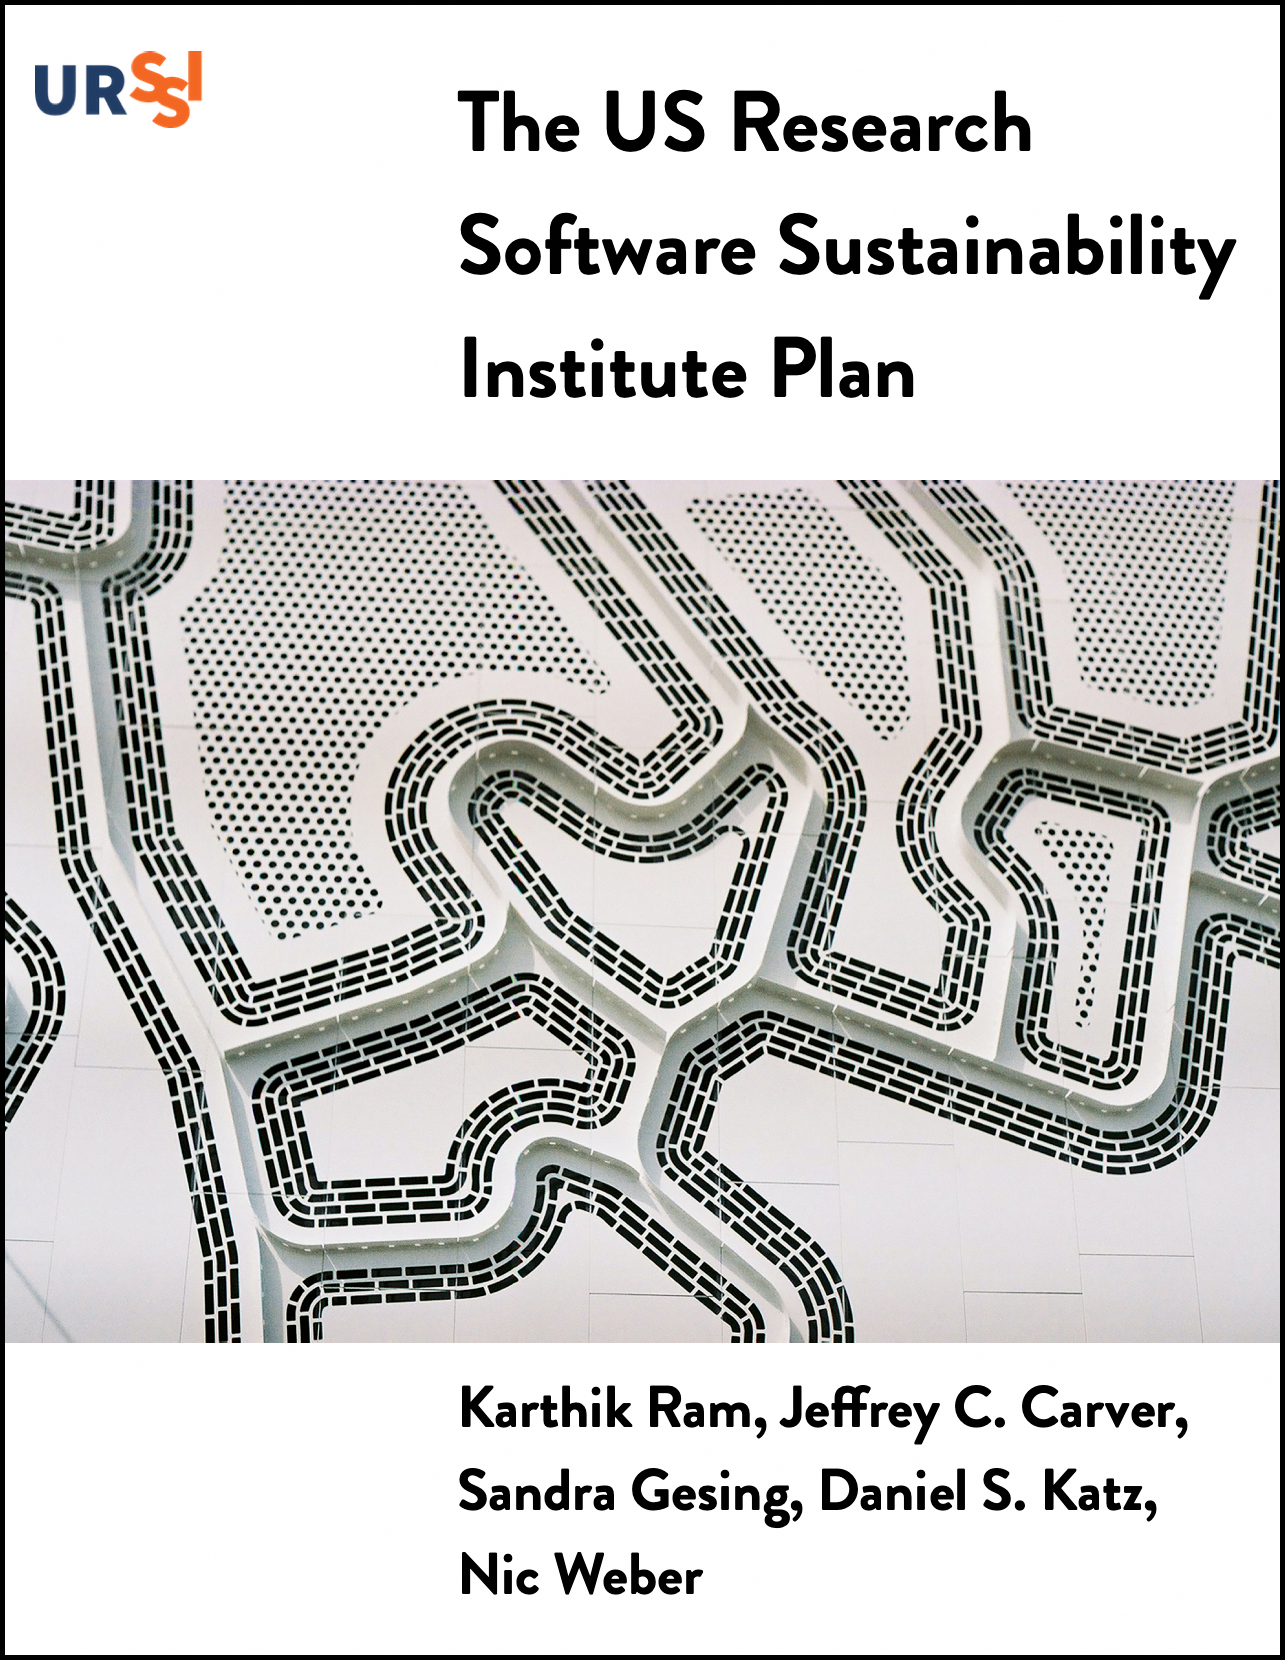
\includegraphics[width=17.85in]{images/plan_png}

This public document is a draft of the final URSSI plan. Empty sections are under internal review before being posted here.

\hypertarget{intro}{%
\chapter{Introduction}\label{intro}}

Software pervades all parts of modern scientific research, including data analysis and inference as well as computational science. One would be hard pressed to find an area of research that is not impacted by software. Recent surveys in the US and UK show that 90-95\% of researchers rely on research software, and 63-70\% of them cannot continue their work if these software were to stop functioning \citep{hettrick2014}. Much of this software is developed by researchers for researchers, as the contemporary scientific process demands the development of new methods in tandem with the demands of new discoveries and fields. However, despite its importance, a large proportion of research software is developed in an ad hoc manner, with little regard for the high standards that are characteristic of other research activities. As a result, the research software ecosystem is fragile and the source of numerous problems that plague modern computational science \citep{carver2018conceptualization}.

Researchers today are under intense pressure to demonstrate expertise in their chosen domains while also trying to maintain a working current knowledge of digital skills such as software engineering.
This combination is unsustainable for most researchers. With little bandwidth to keep up with best practices or sufficient recognition of software development as a scholarly activity, much research software is developed in a manner that makes it wholly unsustainable, despite the obvious role that it plays in modern research, for a multitude of reasons. Academic promotion and tenure, even in institutions with liberal policies, consider peer-reviewed publications to be the primary metric of progress in most disciplines. Even when the impact of software is made clear, it is usually not considered a traditional scholarly activity, making it very challenging to get credit \citep{df80bc12-en}. There is no shortage of horror stories of academics who have built demonstrably impactful software, only to be denied tenure.
Even outside the tenure track, only a few academic jobs offer meaningful career progression for software work. A second reason, strongly correlated with the lack of recognition of software, is the lack of training opportunities. Many research software engineers are self taught. Others learn programming from bootcamps and workshops rather than in traditional academic coursework. Overworked academics are unable to take advantage of such opportunities and therefore develop software using outdated practices. Lastly, even when software is recognized as having impact, funding agencies rarely fund maintenance and ongoing development of such work, leading to reinvention rather than reuse (\url{https://chanzuckerberg.com/rfa/essential-open-source-software-for-science/})

We have spent the last two years engaged in a series of activities designed to gain a
deeper understanding of why research software is so unsustainable and what can be done
about it. Through numerous discussions with diverse groups of researchers, we have
brainstormed challenges and solutions that are highly scalable and impact a large swath
of researchers. This plan discusses the problem in this chapter, describes our activities
(in \protect\hyperlink{chapter2}{Chapter 2}),
outlines high-level plans and methods (in \protect\hyperlink{chapter3}{Chapter 3}),
discusses more detailed plans in the following five chapters
(community \& outreach activities in \protect\hyperlink{Ch-Comm}{Chapter 4},
education \& training activities in \protect\hyperlink{Ch-Edu}{Chapter 5},
incubator activities in \protect\hyperlink{Ch-Incubator}{Chapter 6},
policy activities in \protect\hyperlink{Ch-Policy}{Chapter 7},
and
mangement \& coordination in \protect\hyperlink{Ch-Org}{Chapter 8}),
talks about budget (in \protect\hyperlink{Ch-Budget}{Chapter 9}),
discusses metrics \& evaluation (in \protect\hyperlink{Ch-Metrics}{Chapter 10}),
and then concludes (in \protect\hyperlink{Ch-Summary}{Chapter 11}).
This complete document is the justification and plan for a new institute that will work
in multiple areas to improve research software and the careers of those that produce it,
with an end goal of performing better research.

\hypertarget{nature-of-the-problem}{%
\section{Nature of the problem}\label{nature-of-the-problem}}

One would be hard pressed to name any field of scientific endeavor that has not been substantially transformed by software. From physics to psychology, software has transformed the way we create, acquire, process, model, and draw insights from data. Much of this transformation has come from the increasing availability of open source tools, many of which have helped improve the rigor, quality, and reproducibility of research. The development of research software is often not considered scholarship, making it very difficult for academics to seek funding and find meaningful career paths, especially when research software activities make up a significant part of their contributions. Such people often lead double lives, working tirelessly to meet the traditional responsibilities of academic life, while developing open source tools that enable modern research. We are able to break the problem down into the following four areas:

\textbf{Research software itself is not sustainably developed}: In many fields research software is developed by academics for other academics. Because these people have spent much of their careers developing deep domain expertise, but not developing deep software expertise, software does not often get the same level of care as other aspects of the research enterprise
(\url{https://www.nature.com/articles/s41592-019-0686-2}). Therefore the quality of the software is highly variable, making it hard to sustain. Mounting technical debt often makes it easier to develop software from scratch than to use existing tools. Versions of software used in papers are exceedingly hard to track down, making it challenging to reproduce research findings or reuse research software. When Collberg and colleagues \citep{collberg2014measuring, collberg2015repeatability} decided to measure the extent of the problem precisely, they investigated the availability of code and data as well as the extent to which this code would actually run with reasonable effort. The results were dramatic: of the 515 (out of 613) potentially reproducible papers, across applied computational research, the authors managed to ultimately run only 102 (less than 20\%). These low numbers only count the authors' success in running the code, not in actually validating the results.

\textbf{Lack of career opportunities}: Software does not often count for career advancement (e.g.,promotion and tenure) in academia, making it an invisible scholarly contribution. Research software is often not cited (31-43\%), even in highly ranked journals \citep{howison2016software}. Besides the negative impact on career trajectories, this lack of visibility means that incentives to produce sustainable, widely shared, and collaboratively developed software are lacking. For those outside of traineeships or tenure track positions, the Research Software Engineer (RSE) movement has begun creating a new class of academic positions that explicitly value software work, but such positions are not very common in universities the United States.

\textbf{Lack of training opportunities}: When NSF PIs in the BIO directorate were asked about their biggest challenges in leveraging vast amounts of data currently available, lack of training was listed as the single biggest challenge \citep{barone2017unmet}. Although this training deficit describes the ability to use existing data science software, the skills needed to develop them are harder to come by. While programs like The Carpentries and a handful of university courses offer training in analyzing data, very few train researchers in modern open source software development \citep{Hettrick-blog, hettrick2014, nangia_katz_2017}. This gap remains to be filled.

\textbf{Lack of diversity in research software}: Open source communities struggle to gain participation from women and more broadly from underrepresented groups. Less than 10\% of contributors to open source communities identify as female \citep{Lee2019} compared with approximately 25\% of the overall computer science field \citep{NSF2017, Vasilescu2012}. Cultivating a diversity of perspectives, fields, and backgrounds is important for growing a robust research software community. There is a need to understand the sources of diversity problems and work to improve over the current state \citep{Daniel2013}. Contrary to the initial belief in open source communities, the ability to contribute to a project anonymously does not solve the gender diversity issue \citep{Nafus2012} at least partially because project members are able to determine the gender of contributors, even those that use pseudonyms \citep{Vasilescu2015}. In addition, a large percentage of female contributors have either been subject to or witnessed gender-based discrimination \citep{Powell2010} and have been discouraged from participating in these projects because of the aggressive nature of the discourse and the lack of female role
models \citep{Reagle2012}.
In our own URSSI survey, described in more detail later, we found evidence of the same lack of diversity. When asking survey respondents to self-identify their gender, only 25\% identified as female.
The 164 US respondents to the 2018 International RSE Survey \citep{rse-survey} reported being 82\% male, 14\% female, and 4\% preferred not to say. They also reported being 77\% white, 11\% Asian, 6\% Hispanic/Latino, 5\% other, and 2\% Black. Additionally, 3\% reported having a disability.

\hypertarget{valuing-producers-of-research-software}{%
\section{Valuing producers of research software}\label{valuing-producers-of-research-software}}

Despite the numerous barriers that prevent people from receiving recognition and career success for their research software work, some have successfully overcome them. An exemplar is in this regard is Dr.~Fernando Perez, currently an associate professor in statistics at the University of California, Berkeley. For much of his career he worked in a traditional untenured position as a research scientist in neuroscience and computational research, while collaboratively developing an open source notebook interface for the Python programming language as a side project. Over time, his software work started having much more of an impact than any of his traditional scientific contributions. The current evolution of his group's efforts, the Jupyter ecosystem (\url{https://jupyter.org/}), is considered by many to be ``universally accepted by the scientific community'' and has won him and his team awards such as the \href{https://blog.jupyter.org/jupyter-receives-the-acm-software-system-award-d433b0dfe3a2}{Association for Computer Machinery award for software}.
More recently, the magnitude of his software contributions and the far reaching impact of
this effort (\url{https://www.theatlantic.com/science/archive/2017/06/gravitational-waves-black-holes/528807/},
\url{https://www.theatlantic.com/science/archive/2018/04/the-scientific-paper-is-obsolete/556676/})has earned him a fast-tracked tenured position at University of California, Berkeley. This type of unconventional success in a traditional public university is a sign that the recognition of software work as scholarship is changing.

While the result of Dr.~Perez' story is promising, it is very difficult to achieve. Other academics who have produced work of similar or greater magnitude in the past weren't as fortunate. Travis Oliphant, for example, served as an assistant professor of Electrical and Computer Engineering at Brigham Young University in the early 2000s. Among his accomplishments during this time, he is credited as the primary creator of NumPy, the Python library for numerical arrays that is the foundation of modern data science tools, and as one of the early contributors to SciPy, the widely used library for scientific Python. These contributions were deemed insufficient for tenure. Kirk McKusick, a professor at EECS in Berkeley was denied tenure in the early 1990s because his primary work was on the BSD Software Project, which then went on to become the foundation of the modern internet. {[}\textbf{TODO}: Other examples would be welcome and appreciated. Are there women/people of color who have experienced similar situations that we can highlight here?{]}

\hypertarget{why-we-ran-this-conceptualization}{%
\section{Why we ran this conceptualization}\label{why-we-ran-this-conceptualization}}

It comes as no surprise to researchers that software is undervalued in academia. However, substantive evidence supporting this claim is scattered and mostly anecdotal, making it hard to build a convincing case that the research community and their stakeholders need to care more. In 2017 we submitted a proposal to the National Science Foundation's \href{https://www.nsf.gov/pubs/2015/nsf15553/nsf15553.htm}{Software Infrastructure for Sustained Innovation (S2I2) program} to gather this evidence, identify unique challenges not already being addressed, and to formulate a plan for an institute to implement solutions. The proposal was funded in December 2018, allowing us to engage in various activities over the following 24 months. Despite the awareness of these issues and the existence of similar conceptualizations (albeit domain-centric ones), the core challenges around sustainability (of people/software/practices), recognition and credit, and training/workforce development remain poorly understood and poorly addressed.

We used a wide range of approaches to understand the core social and technical challenges of developing sustainable research software. These approaches include an extensive survey, in-person unconferences, both general and topic focused, a pilot training event, and a series of ethnographic studies. We mapped out the current state of software related challenges with an extensive survey targeting researchers across the country. We also invited participants to workshops across the country to share critical challenges and brainstorm solutions in small groups. We dug deeper on a couple of core issues that arose repeatedly (credit and incubators) by organizing two focused workshops to tackle them (credit and incubators). This report captures our summary of the survey, workshops, and studies and describes a core set of activities that define the work of a future US Research Software Institute.

\hypertarget{what-we-plan-to-do-and-why}{%
\section{What we plan to do and why}\label{what-we-plan-to-do-and-why}}

The conceptualization phase with its survey, workshops, and ethnographic studies elucidated the need in the community for different components of a potential implementation of URSSI. We identified four areas for supporting the research software community - to accelerate science for diverse research domains as well as software engineering as a research area in its own right. Each of these activities contributes to the desired impacts described in \href{https://plan.urssi.us/chapter3.html\#desired-impact}{Section 3.4}.

\begin{enumerate}
\def\labelenumi{\arabic{enumi}.}
\item
  \textbf{Incubator}: Sustainability of research software has many aspects beyond good software engineering practices that overlap with diverse areas of expertise. Such areas include technology advice, project management, business planning, usability advice, license management, etc. The incubator service area would focus on providing projects with experts who have a consultancy agreement and could support a project in the different stages of their life cycle -- from spinning up a project to first results and uptake of software to planning its sustainability after the funding ends.
\item
  \textbf{Education \& Training}: Many universities offer curricula in conceptual software engineering but there is a lack of practical training to meet the community needs to go into depth for different technologies. University courses offered in computer science departments are also often impractical for domain researchers. The survey showed that there is a need to choose formats and timeframes that are suitable for people in the role of Research Software Engineers (RSEs) and busy domain scientists who lack formal or informal training. While The Carpentries and the \href{https://codata.org/initiatives/strategic-programme/research-data-science-summer-schools/}{RDA-CoDATA summer school}, for example, do an excellent job of teaching basic programming and computational \& data analytic methods to researchers in a peer-to-peer model, mostly in 2-day courses, URSSI has a massive opportunity fill the gap in teaching more in-depth software engineering, software project management, and community development practices in longer engagements, such as a 5-day summer- and/or winter-school. URSSI will strive to collaborate on topics with the Carpentries and the existing software sustainability institutes, such as the Science Gateways Community Institute and the Molecular Sciences Software Institute, so that rather than replicate effort, identify training opportunities in the overall research software landscape that is currently missing.
\item
  \textbf{Policy}: Policy is an important area to improve the sustainability of research software. Policies could include campaigns as well as guidelines for citation of software, templates for job positions, good software engineering practices as well as bad software engineering practices as counterexamples. We have already been collaborating with the UK SSI for several years and plan to expand collaborations with initiatives/projects such as US-RSE to find a common ground on international level while considering the specific situation in the US.
\item
  \textbf{Community \& Outreach}: Many researchers or developers in the role of an RSE work in silos and the Community \& Outreach area of URSSI would connect them to peers and provide access to beneficial material, resources, and contacts to improve this situation. The RSE community has already achieved some successes by simply working together. The number of chapters has gone from 1 UK university in 2013 to 28 chapters in 2020. URSSI has the potential to capture more of this momentum. Community engagement would include scalable communication such as a website, blogs and newsletters, two-way communications for discussions such as webinars and online discussion forums as well as face-to-face meetings in the form of workshops. In addition, this area will include a fellows program to support work done by community members that benefits URSSI activities.
\end{enumerate}

Building these different areas into URSSI would formalize URSSI's informal position as the focal point for the overall community of software developers as well as for a set of disciplinary communities. URSSI will help accelerate science that needs research software and improve the career paths of those who develop and maintain it, including RSEs.

\hypertarget{chapter2}{%
\chapter{URSSI Conceptualization}\label{chapter2}}

The purpose of this conceptualization project was to create a roadmap for a US
Research Software Sustainability Institute (URSSI). The roadmap was to be
informed by and responsive to a community of potential stakeholders, including
researchers, software developers and users, funders, and program / product managers.
To engage this diverse group of people and institutions we completed the
research described in this section including a series of workshops, community outreach and
communication, a survey, set of ethnographic studies, and a pilot Winter School
for early-career researchers. At the conclusion of this section we offer a
summary of the challenges identified, collectively, across all of the URSSI
conceptualization activities and what role we believe URSSI should play in
addressing these challenges.

\href{https://plan.urssi.us/images/conceptualization_activities.jpg}{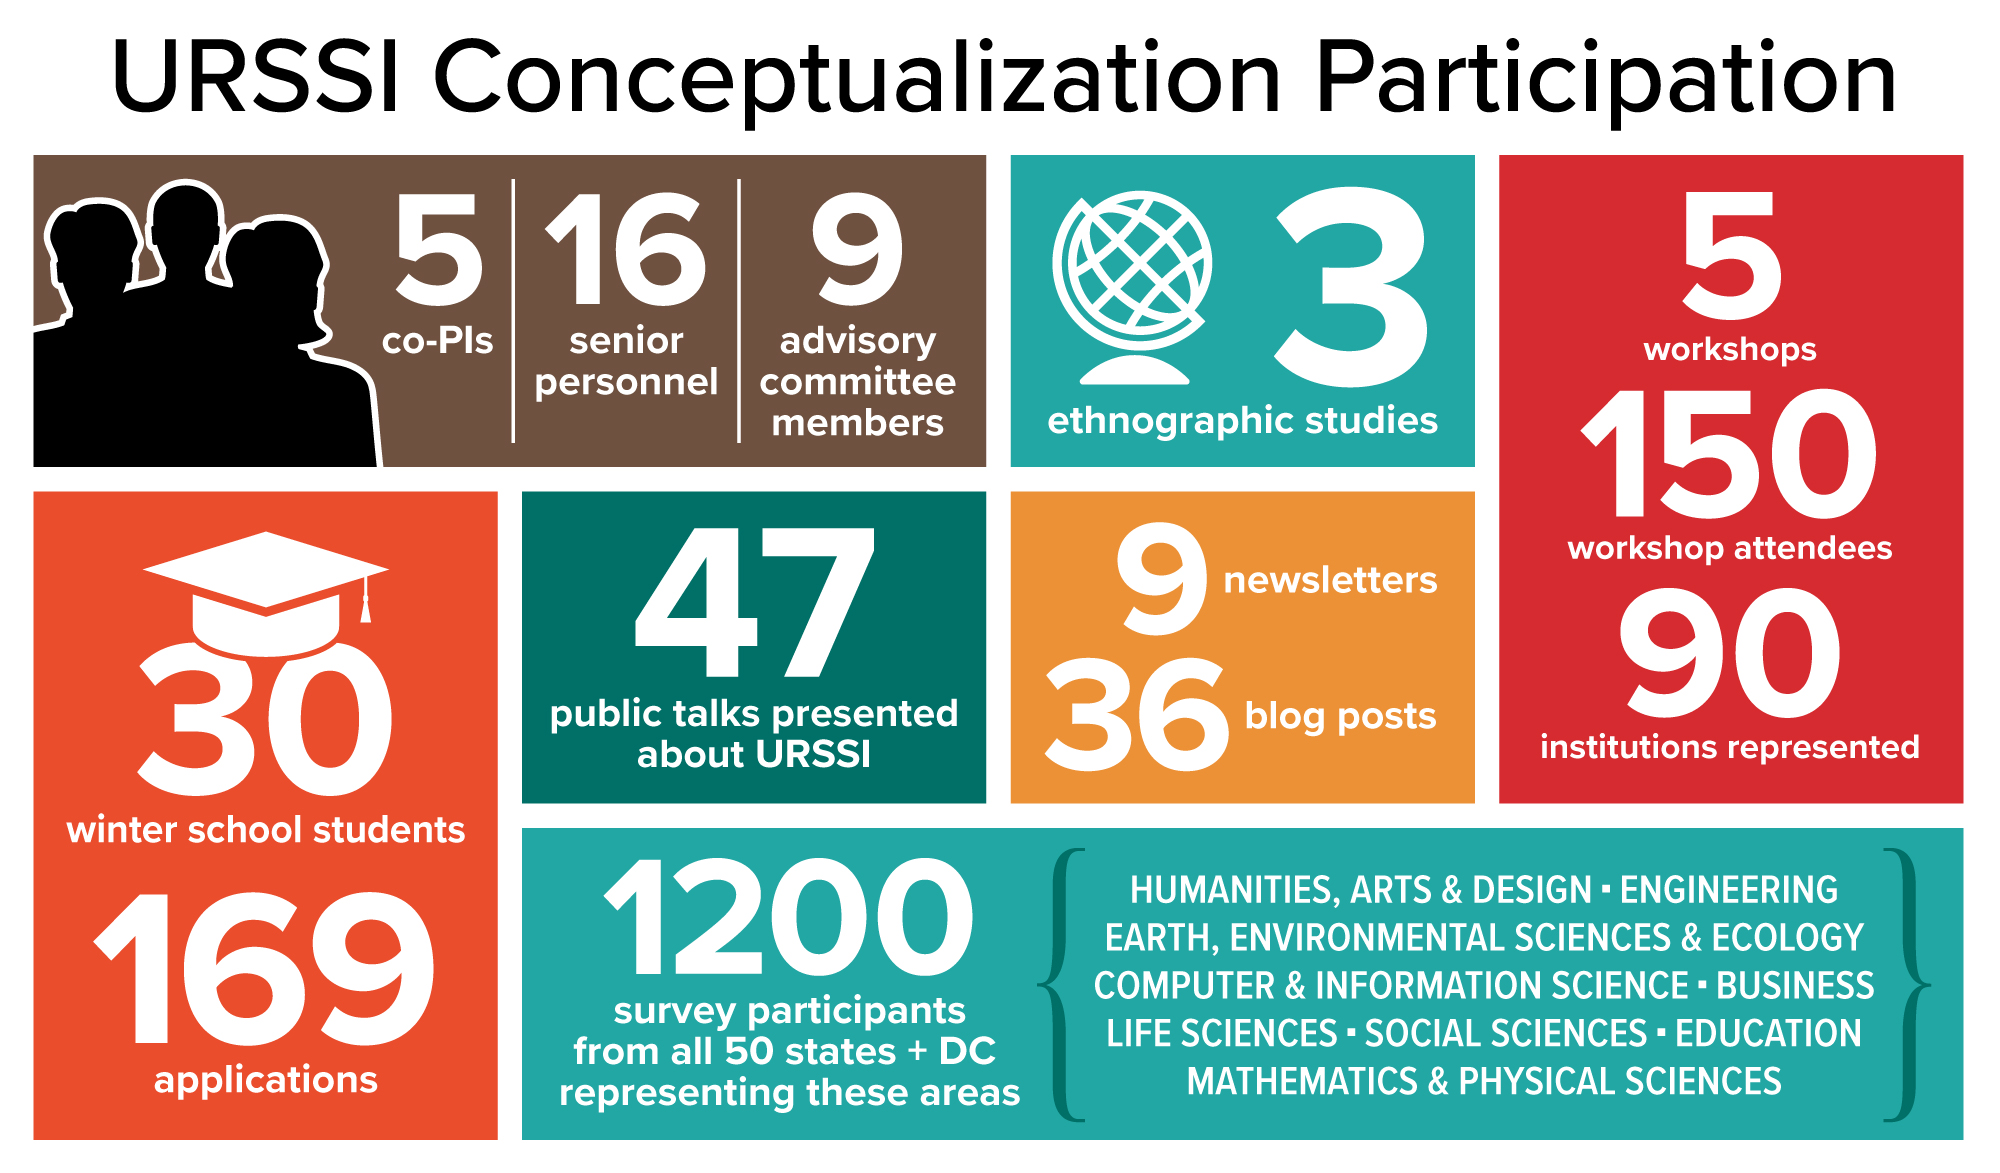
\includegraphics{images/conceptualization_activities.jpg}}

\hypertarget{workshops}{%
\section{Workshops}\label{workshops}}

\textbf{Community wide workshops}: In 2018 we held two community workshops with
URSSI stakeholders in Berkeley (April) and Chicago (October). We invited participants
based on their ability to represent diverse roles, institutions, and
perspectives on research software. The general goal of the two community workshops
was to determine which topics this diverse group of stakeholders consider to be
well-understood, which topics still have uncertainty or a need for guidance, and what work
remains to be done in supporting sustainable research software. URSSI PIs
facilitated broad discussions and participated in small group breakout
discussions. Additionally, participants at each workshop gave presentations
about their on-going research software activities.

\textbf{Thematic Workshops}: Participants at the first community workshop identified
two topics worthy of more focused discussion and community input.
We organized the following workshops to better understand those topics:

\begin{itemize}
\item
  The \textbf{Metrics, Credit and Citation Workshop}, held in Santa Barbara,
  California in January 2019, focused on reseach software metrics, citation,
  and impact evaluatin. The 23 participants had strong expertise in the
  various workshop themes, including the PIs of the CodeMeta project, Zenodo,
  and software credit initiatives such as SourceCred.
\item
  The \textbf{Research Incubators Workshop}, held in College Park, Maryland
  in February 2019, focused on methods for incubating new and existing research projects.
  The 20 participants had strong expertise in
  research software project development, including program officers from
  various government agencies, open-source research software developers,
  and organizational scholars that have studied research software processes.
\end{itemize}

\textbf{URSSI Design Workshop}: In April 2019 members of the Senior Personnel
and Advisory Committees participated in a workshop in Chicago, IL. PIs
presented preliminary results from our research (ethnographies and survey)
as well as lessons learned from the four previously held URSSI workshops.

\hypertarget{website-newsletter-blog}{%
\section{Website / Newsletter/ Blog}\label{website-newsletter-blog}}

One of the major goals of the conceptualization project was to build awareness
of the need for an institute, publicize our activities, and increase overall community interest.
To achieve this goal, we used a \href{http://urssi.us}{website}, nine \href{http://urssi.us/newsletter/}{newsletters},
36 \href{http://urssi.us/blog/}{blog posts}, and a seires of public talks and webinars given
by the PIs and others. We sent the newsletters to the URSSI email list, which consists
of workshop attendees and other interested members of the community.
We also publicized the newsletter and blog posts via the \href{https://twitter.com/si2urssi/}{URSSI twitter account},
which has over 500 followers.

\hypertarget{survey}{%
\section{Survey}\label{survey}}

We developed and disseminated a survey to compliment workshop participation.
The primary goal of the survey was to gather the opinions, preferences, and
self-reported activities of the research software community regarding
development practices, development tools, training, funding/institutional
support, career paths, credit for software work, and diversity/inclusion.
For each of these topics, we asked a small number of general questions and
then allowed participants to self-select to answer more detailed questions
about any area of particular interest. We distributed the survey to PIs of
currently funded NSF and NIH projects and to relevant mailing lists. The
survey closed in May 2019 after receiving approximately 1200 responses.

The results of the survey highlighted some areas where URSSI could play a
key role in advancing the sustainability of research software in the United States.

\begin{enumerate}
\def\labelenumi{\arabic{enumi}.}
\item
  There was a mismatch between how respondents wanted to allocate their
  time and their actual allocation of time. This result provides an opportunity
  for URSSI to work with developers and teams to help them focus their efforts
  on the tasks that are most relevant.
\item
  The aspects of the software development process respondents viewed as
  being more difficult than they should be tended to be people-related
  activities rather than technical activities. This result suggests that URSSI
  could support teams and developers by providing training and/or
  resources related to human factors in the software development process.
\item
  Respondents indicated they use a number of software development practices.
  However, one key practice that was underutilized is peer code review. URSSI
  can provide training on peer code review and work with teams to ensure that
  the infrastructure is in place to appropriately support this activity in the
  research software space.
\item
  The respondents indicated that software development practices including
  \emph{requirements}, \emph{design}, \emph{maintenance}, and \emph{documentation} were not
  well-supported by tools.
\item
  In terms of version control, there is still a sizable percentage of
  people who use methods like \emph{copying files to another location} and
  \emph{zip file backups} as version control. This result suggests that URSSI
  could provide additional training and tools to help teams use modern
  version control systems.
\item
  Many of the items above relate to training, or the lack thereof. The
  survey results suggest a large percentage of respondents have not received
  training in software development. While the respondents indicated there were
  sufficient opportunities for training, most of them suggested they did not
  have sufficient time for training. URSSI could help by providing training
  in different formats that work better with the demands of the research
  software developers' environments.
\item
  Many respondents also found the level of support, in terms of funding,
  to be inadequate to be successful. URSSI could help by advocating both at
  the national funding level as well as at the University level for increased
  funding for important research software development activities.
\item
  Respondents also indicated their software contributions were not
  significantly valued in performance reviews. URSSI could help by developing
  and advocating for policies that help research software developers get
  adequate recognition for their work.
\item
  Most projects lack a formal diversity plan. URSSI could help by providing
  template diversity plans and support for developing
  appropriate plans for individual projects.
\end{enumerate}

\hypertarget{ethnography}{%
\section{Ethnography}\label{ethnography}}

To gain a deeper understanding of the practices and experiences of researchers
who are actively engaged in software development, we have undertaken a series of
ethnographic studies. These studies focused on software projects of varying
size and complexity in the fields of hydrology, astronomy, and biochemistry.
Using observations, semi-structured interviews, and a
series of archival documents, we produced case studies of how, over time, these
projects overcame challenges of recruiting contributors, building a governance
model, seeking funding, and sharing credit in sustaining a software project that
has demonstrable impact on a community of researchers.

We developed two of these studies, Astropy and Rosetta Commons, as full case
studies. Both projects face unique sustainability challenges that they solved
somewhat differently. While the main findings of this work are not novel
in the sense that they will surprise anyone familiar with challenges to sustaining
research software, the value of this work is in comparing the two cases. By better
understanding common approaches to overcoming sustainability challenges, we believe
there is a valuable opportunity to abstract these approaches into models of success
that research software projects in other domains can modify or tailor.
The following is a brief summary of the findings from these two case studies.

Points of comparison:

\begin{itemize}
\item
  \emph{Distributed work coordination}: Key to the success of both Astropy and Rosetta
  Commons is coordination of remote collaborative work. Astropy mirrors Python's
  core development team in structuring contributor guidelines and supporting
  designated maintainers. Rosetta Commons differs substantially in that the project
  employs four full-time infrastructure maintainers. This offloading of
  maintenance responsibilities frees up contributors (distributed labs throughout
  the USA) to focus on conducting research and driving innovations that extend
  Rosetta's key functionality.
\item
  \emph{Funding}: Astropy is fiscally sponsored by NumFocus, but depends upon grant
  funding from a variety of sources to sustain its collective work. A recent
  grant from Gordon and Betty Moore Foundation, ``Sustaining and Growing the
  Astropy Project,'' is focused exclusively on maintenance and governance for
  the project's long-term viability to practicing astronomers. Rosetta Commons
  combines licensing and grant funding to sustain its work. Licenses for
  commercial use and an NIH infrastructure maintenance grant have continuously
  supported the project since 2005.
\item
  \emph{Credit}: Both projects have had a number of papers published about their
  development. Astropy suggests two publications to cite when acknowledging
  use of the software \citep{robitaille2013astropy, price2018astropy}. These two
  publications, combined, have over 3000 citations. Rosetta Commons,
  because it has many versions, methods, and language specific implementations,
  has no canonical citation. Interviews with contributors to Rosetta noted
  that this lack of canonical citation causes confusion for authors when rushing towards publication.
  Many researchers have sought a centralized source they could acknowledge.
  Despite the lack of a canonical citation, two papers describing Rosetta and
  its use in predicting protein structures have, combined, over 4300
  citations \citep{rohl2004protein, salmena2011cerna}.
\end{itemize}

We observe differences in the two projects that seem marginal at first
glance, but upon further analysis have important practical consequences
for software development activities. For example, two substantial
differences in the projects have consequences for the long-term sustainability
of each project:

\begin{itemize}
\item
  Astropy, in following an open model of contribution, focuses time and
  attention on clearly documenting and making contributor guidelines
  accessible to research software engineers. The maintenance team
  therefore focuses their effort on ensuring contributors are supported
  while simultaneously keeping various packages up to date and available
  to the community that depends upon this code for their research. This approach is
  partially a result of the software ecosystem being broadly useful to a
  discipline (Astronomy), as compared to Rosetta Commons, which focused on
  specific analytic tasks within a subfield of biological engineering
  (Macromolecular modelling).
\item
  Continuous annual grant funding and licensing fees allow Rosetta to
  centralize infrastructure tasks to a core team whose sole job is
  maintenance. This approach in turn encourages innovation and expansion of feature
  sets for labs that focus solely on producing new research insights.
  Astropy has, over time, centralized maintenance of the project's software
  development and maintenance. But until very recently, this maintenance has been a
  volunteer activity. Shifting time, attention, and energy towards organizing
  an open-source model of development impacts career trajectories for
  practicing astronomers and contributes to a more fragile ecosystem for astronomy.
\end{itemize}

We recognize that software sustainability is more than just financial support,
but what these case studies make clear is that the economic realities of
maintaining and contributing to software development have important downstream
impacts that shape innovation and engagement. The URSSI conceptualization
has studied how these challenges can be practically overcome.

\hypertarget{chapter2-WinterSchool}{%
\section{Winter School}\label{chapter2-WinterSchool}}

In late December 2019 we ran our
first ever URSSI school on research software engineering. We began accepting
applications in July and received an overwhelming response to our call for
applications. For the 30 participant slots available, we received 169
applications, meaning we had a challenging time selecting the participants
and had to turn away a large number of interested researchers. While the
selection committee used multiple criteria to evaluate and select participants,
successful applicants already had some experience with Python programming, Git,
and Unix skills, which was necessary to benefit from the workshop. Our goal
was not to repeat the same material covered in bootcamps and Software Carpentry
style workshops, but to focus on the research software engineering skills that
not formally taught in any setting. These skills include best practices
for packaging code as software, testing, collaborative software development,
code review, and related topics such as licensing and archiving. The school
lasted 2.5 days.

Based on the demand described above, this experience made evident the strong
need for the skills covered in the school. The overall feedback from the
school was also positive (more on that below). Some key lessons from this
pilot that impact our design of a Summer School as part of URSSI are: 1) the
school needs to be longer to allow for both discussion time and focused time
for students to work on their own code, applying the lessons from the lectures;
and 2) the presence of additional helpers outside of the primary instructors was
quite beneficial to help answer specific questions from the students.

A few example quotes from the Winter School feedback form include:

\begin{itemize}
\item
  ``I really can't say enough good things about this super empowering workshop!
  You did an amazing job identifying the things I didn't know that I didn't know,
  and teaching them at a level that was immediately actionable in my work.''
\item
  ``Thank you so much to everyone for taking this amazing initiative to teach young
  scientists on software sustainability.''
\item
  ``Thank you for putting together this winter-school, it was super useful to me
  and I'm looking forward to applying everything I learned to my future projects
  and to go deeper into the topics that were covered.''
\end{itemize}

\hypertarget{joint-activities}{%
\section{Joint Activities}\label{joint-activities}}

During the URSSI conceptualization process, we helped start two new activities that
overlapped our goals, both so that we could promote these goals and also so
that we could build up these future partners of a later full URSSI institute.

\hypertarget{research-software-alliance-resa}{%
\subsection{Research Software Alliance (ReSA)}\label{research-software-alliance-resa}}

\href{http://www.researchsoft.org}{ReSA} was founded in 2018 to support recognition and valuing of research software as a
fundamental and vital component of research worldwide, instigated by URSSI,
the UK \href{https://software.ac.uk}{Software Sustainability Institute},
and the \href{https://ardc.edu.au}{Australian Research Data Commons}.
ReSA's mission is to bring research
software communities together to collaborate on the advancement of research software.
Recent achievements include:

\begin{itemize}
\item
  Development of research software guidelines for policy makers, funder, publishers and
  the research community for inclusion in the RDA COVID-19 Guidelines and Recommendations \citep{RDA-covid-recs-final}
\item
  Inclusion of software in the draft revision of the OECD Committee for Science and Technology
  Policy's Enhanced Access to Publicly Funded Data for Science, Technology and Innovation (which will become soft law) (\textbf{TODO} add link to final document after release)
\item
  Co-leadership of the \href{https://www.rd-alliance.org/groups/fair-4-research-software-fair4rs-wg}{FAIR 4 Research Software taskforce}
  with \href{https://www.force11.org/}{FORCE11}
  and \href{https://www.rd-alliance.org/}{RDA} to develop community-agreed principles and implementation guidelines
\item
  Support from the Gordon and Betty Moore Foundation to achieve ReSA's goals
\end{itemize}

The Director of ReSA is Michelle Barker and the Steering Committee is comprised of:

\begin{itemize}
\tightlist
\item
  Neil Chue Hong, Director, Software Sustainability Institute, UK
\item
  Catherine Jones, Software Engineering Group Leader, STFC, UK
\item
  Daniel S. Katz, Assistant Director for Scientific Software and Applications, National Center for Supercomputing Applications (NCSA), University of Illinois, USA
\item
  Chris Mentzel, Executive Director, Stanford University, USA
\item
  Karthik Ram, URSSI PI, University of California, Berkeley, USA
\item
  Andrew Treloar, Director, Platforms and Engagements, Australian Research Data Commons, Australia
\end{itemize}

\hypertarget{research-software-engineering-rse}{%
\subsection{Research Software Engineering (RSE)}\label{research-software-engineering-rse}}

In a 2012 workshop run by the UK SSI, a number of UK researchers who develop
software realized that while they internally recognized a number of common elements
to the work they did, along with others at their universities, there was no
commonality to how others saw this work and these roles, and they needed to come
together to build and develop a community. As stated by James Hetheringon, they
decided they needed to ``develop the profession of a scientific software engineer
and the career track of software developers in academia.'' The SSI studied academic job
descriptions in the UK, and found about 10000, of which about 400 were related to
software development, with 194 different job titles. To build recognition of the
common software elements of these positions, the SSI chose the name ``research software
engineer''. The SSI then began publicizing this idea, building a community of people who
identified with the role, leading to the formation of the UK RSE Association, which is
now the \href{https://society-rse.org}{Society of Research Software Engineering}.
The SSI and RSE Association/Society encouraged people who were performing RSE-like work
to also identify with this title,
built RSE groups in UK universities, encouraged universities to change their
job titles, held workshops and then conferences for RSEs, encouraged a funding
agency to provide fellowships to RSEs, and built up the association/society,
which now has about 2000 members \citep{RSEHettrick}.

As a number of non-UK people (including some URSSI PIs) started attending UK RSE
conferences, the SSI also supported activities to grow the international community.
These self-developed and SSI-supported activities have led to RSE groups in Germany,
the Netherlands, the Nordic countries, the US, Canada, Australia/New Zealand, South Africa, and Belgium, some of
which have now held national workshops and conferences. The US Research Software
Engineer Association (US-RSE) formed in 2018, with the support and participation
of three of the five URSSI PIs, and has 420 members as of May 2020. The US-RSE
Association is centered around three main goals:

\begin{itemize}
\item
  \emph{Community}: to provide a coherent association of those who identify with the role
  (not necessarily title) of Research Software Engineer, and to provide the members
  of the community the ability to share knowledge, professional connections, and resources.
\item
  \emph{Advocacy}: to promote RSEs' impact on research, highlighting the increasingly
  critical and valuable role RSEs serve.
\item
  \emph{Resources}: to provide useful resources to multiple demographics, including technical
  and career development resources, and information and material to support the
  establishment and expansion of RSE positions and groups within the research ecosystem.
\end{itemize}

There are thus some overlaps between US-RSE's goals and URSSI's and a clear reason
for us to work together going forward.

\hypertarget{synthesis-of-urssi-activities}{%
\section{Synthesis of URSSI Activities}\label{synthesis-of-urssi-activities}}

In the following section we describe common challenges and dilemmas we
identified across URSSI's conceptualization activities. Where possible, we identify
the role URSSI could play in helping overcome these challenges as a funded institute.

\textbf{Challenge 1: Decentralized expertise}

Throughout the planning activities, the community of stakeholders recognized
that there already exist a number of individual efforts to help improve the
development, maintenance, and overall sustainability of research software in
the US. While these efforts, collectively, are comprehensive in their scope,
the decentralized structure of this expertise is inefficient for both resource
discovery and delivery of services. For example there are many points of expertise
in research software development (e.g., SWEBOK, RSEs), education and training
(e.g., academic initiatives, Carpentries), credit and metrics (e.g., CiteAs),
incubation (e.g., ESIP, the UW eScience Institute) that are available to
individuals at specific institutions. However, there is currently no comprehensive
organization that can serve to coordinate these activities, promote centers of
expertise, and ensure that effort is not duplicated-- a role that is played
admirably in the UK by the Software Sustainability Institute.

As a coordinating center, URSSI could help solve this challenge in the following ways:

\begin{itemize}
\item
  Broker connections between points of expertise and serve to coordinate
  efforts and funding such that different experts could better collaborate on
  sustainable development, education, and policy initiatives.
\item
  Identify and convene experts to help fill gaps that exist between service
  delivery, for example, where the Carpentries see gaps in knowledge skill or
  acquisition in sustaining software education.
\item
  Disseminate best practices from specific disciplines to the broader
  research community. By acting as a center of research software excellence
  URSSI could be a space where solutions from one domain could be learned and
  efficiently transferred to another.
\item
  Coordinate and help to curate relevant research software packages through
  discovery portals, such as \url{https://libraries.io/}
\end{itemize}

\textbf{Challenge 2: Pathways to sustainability for non-commercial research software}

Throughout the URSSI conceptualization activities, participants voiced concern
for the viability of valuable software projects that do not seek
commercialization. Technology transfer programs at universities and through
research funding agencies (e.g.~I-Corps, SBIR/STTR) are well established
and have been successful at helping entrepreneurially-focused software projects
recognize and execute viable business models. This transition pathway is
promoted for software that has a potential to sustain itself through fees or
licensing agreements. However, there is no equivalent university guidance for
software projects that would like to pursue non-commercial open source models
for sustainability.

There is a need for a US-based institute, divorced from any single university,
to help valuable research software projects realize a non-commercial
open-source route to sustainability. This support could include a program, such as an
incubator, that would guide research software projects towards developing
open-source governance, budgeting, licensing, and fiscal sponsorship in service
of non-commercial sustainability. We view this route, and its guidance from an
institute, as critical to promoting an ecosystem of diverse research software
projects that may not be readily amenable to commercialization, or have the
potential to build healthy and viable volunteer developer communities as an
alternative to licensing.

\textbf{Challenge 3: Coordinated advocacy and analysis for policy change}

Related to the first challenge of decentralized expertise, there is a need
for coordination and targeted leadership around policy for sustainable
research software. Participants in URSSI workshops described a need for
coordinating communities around emerging national, institutional, and even
disciplinary specific policies that have a downstream impact on sustainability,
such as software citation principles, tenure and promotion guidelines that
recognize research software contributions, sustained funding or financial
support for research software maintenance, and software management plans
that explicitly document expectations around software development and archiving.

Currently, community members take on many of these policy activities as additional
professional service, or as volunteer work. This secondary focus on any
one policy issue, in turn, leads to slow progress, high turnover of volunteers,
and does not allow any one person or institution to develop the deep expertise
needed for effective sustained analysis or advocacy.

An institute that could dedicate time and attention to policy design, invest
personnel time in developing needed expertise, and coordinate a sustainable
lobbying network would allow advocacy work to become more manageable,
effective, and result in better outcomes for research software stakeholders.
Further, there is often a need to conduct advocacy work driven by
empirical research that can substantiate how or why one policy decision is
better than another. An institute dedicated to these activities would
facilitate data-driven policy research that could lead to stronger advocacy
positions, and benefit funding agencies, universities, and research
institutions that seek to adopt new policy aimed at improving research
software sustainability.

\textbf{Challenge 4: Signals of viability}

A valuable contribution of the URSSI workshop and engagement activities has
been convening stakeholders with expertise in the evaluation and funding of
research software. These stakeholders include current and former program officers
from NSF, NIH, DoE, DoD, and IMLS, as well as philanthropic organizations
like the Gordon and Betty Moore and Alfred P. Sloan foundations. These
participants have a collective desire for an institute to develop stronger
signals of a research software project's viability; to help evaluate a
project's potential for long-term sustainability; and help communities of
research software stakeholders coalesce around strategic funding initiatives
that could benefit research through software investments.

A dedicated US institute focused on software sustainability could help meet
this challenge in a number of ways, but we recognize that there is no
overarching or simple solution. The plan we describe below explains,
in numerous places, how URSSI can and should convene different communities
to address complex problems like strategic financial investment, evaluation
for viability, etc.

\textbf{Challenge 5: Career Advancement and Credit}

Closely related to Challenges 1, 3 and 4 is a desire of URSSI stakeholders to
see an institute dedicate time and resources towards promoting recognition
for research software activities and helping to shape reliable career pathways
for research software engineers (RSEs). At URSSI workshops, there was
near-unanimous agreement that the acknowledgement of research software
contributions remains difficult for career advancement and there is a lack
of clear guidance for both universities and funding agencies on how to make
progress on these issues.

A dedicated US-based institute for research software sustainability could
play a leading role in advocating for best practices in the measurement,
reward, and credit for research software activities. This activity would include
dedicated research into measuring and evaluating software development activities,
advancing techniques for use and user impact evaluation, and promoting formative
metrics that are conducive to long-term viability. Relatedly, a dedicated US-based
institute could better evaluate and promote the impact of research software
engineering positions that currently exist and advocate for their creation
where they do not.

In the next chapter, we describe URSSI's plan to meet each of these challenges.
In particular, we focus on how a strategic investment in a US-based software
sustainability institute would practically organize itself, allocate budgets,
and measure progress on each of the challenges identified in the conceptualization phase.

\hypertarget{chapter3}{%
\chapter{URSSI Plan}\label{chapter3}}

Throughout the URSSI conceptualization process, the team worked on overall
planning iteratively, using slides at workshops and the URSSI website to
disseminate current thoughts, using the survey and the ethnographic studies as
inputs, using workshops (including slides and shared note documents) and the
discussion forum (using Discourse on \url{https://discuss.urssi.us}) to gather and record feedback. Together,
these activities plus internal discussions of the team and a focused mission and
vision working group have led to most of the content of this document.

\hypertarget{mission-and-vision}{%
\section{Mission and Vision}\label{mission-and-vision}}

URSSI PIs began to develop mission and vision statements in late 2018. The intent
of these statements was to succinctly state the purpose for URSSI's existence
(mission) and based on that purpose what URSSI strives to achieve (vision). The
process for developing these statements was:

\begin{itemize}
\item
  At the first two workshops, we asked participants about the goals and vision
  that a US research software sustainability institute should pursue.
\item
  The URSSI PIs then identified institutions with similar goals and collected
  their mission and vision statements for comparison.
\item
  Eight members of the Senior Personnel and Advisory Committee participated in
  a working group focused on developing URSSI's mission and vision statement.
\item
  Each working group participant provided a written set of three mission and
  three vision statements based on the conceptualization proposal, workshop
  participant's feedback, and guidance from the URSSI PIs.
\item
  Neil Chue Hong, director of the Software Sustainability Institute in the UK,
  facilitated a synthesis of the working group's feedback. This synthesis process included a
  teleconference with participants to discuss and refine versions of each
  mission and vision statement.
\item
  The URSSI PIs then presented drafts of each statement to workshop participants
  at the final URSSI meeting in Chicago and refined a final version of each statement.
\end{itemize}

The mission and vision of URSSI are as follows:

\textbf{Mission}: Our mission is to improve the recognition, development, and use of
software for a more sustainable research enterprise. We achieve this mission
through collaboratively developing education, outreach, and software services
that emphasize open, transparent reproducible, and cooperative practices. URSSI
is an institute for software expertise as well as a social infrastructure that
promotes an inclusive and diverse community of research software engineers,
maintainers, contributors, and users.

\textbf{Vision}: Empowered people, building better software, enabling exceptional research

\hypertarget{planning-assumptions-methods-and-principles}{%
\section{Planning assumptions, methods, and principles}\label{planning-assumptions-methods-and-principles}}

The following assumptions are inputs to our planning process:

\begin{itemize}
\item
  Our plan is based on the idea of proposing to NSF, and therefore, focuses on the
  US community. We will, however, work with like-minded organization both inside and
  outside the US, including the \href{https://www.researchsoft.org}{Research Software Alliance (ReSA)}.
  (Also see the potential partners listed the next subsection.)
\item
  We will propose an institute with a 5-year duration and a potential 5-year
  extension, based on NSF's current institutes and published documents.
\item
  The budget of URSSI will be \$3m-\$5m per year. We take \$3m as the baseline
  minimum funding level needed to operate an institute, below which an institute
  is not the right method to achieve the mission and vision, and then build higher
  cost and higher return activities on that baseline.
\item
  There is demonstrated interest in supporting some URSSI goals from private
  foundations and potential interest from other federal agencies, so URSSI
  activities should be planned as a set of reinforcing (but separable) activities,
  potentially on different timelines.
\item
  There is a strong need for improved software sustainability across all fields,
  and URSSI cannot solve this need in all fields by itself.
\item
  There are many partners who can help URSSI achieve some of its goals, as there
  is overlap between these goals and the goals of those partners (see the next subsection)
\item
  It is not practical for URSSI to directly work with the US research software development
  community (all of those who develop research software in the US, including in academia,
  national laboratories, and industry) due to the small size of URSSI and the very large size of this community, so
  URSSI needs to work indirectly by leveraging other groups.
\end{itemize}

Given the mission and vision, and our assumptions, we plan to use a set of methods
to ensure that URSSI is successful:

\begin{itemize}
\item
  URSSI must choose a set of initial targeted communities and efforts, focus on
  them for some period (until some predefined metrics of success are met or some predefined
  time period has passed without success), then move on to the next set of targets
\item
  URSSI must work closely with partners to amplify its efforts (see the next subsection)
\item
  URSSI must be clever about using resources, attempting to achieve multiple outputs
  for activities whenever possible.
\end{itemize}

Guiding principles:

\begin{itemize}
\item
  Leverage existing organizations for authority, credibility, resources
\item
  Focus on people, not projects
\item
  Embed diversity and inclusion within all aspects of URSSI
\item
  Leverage available resources (software, services, credit systems, training
  materials, etc.) where possible rather than reinvent
\item
  Share resources we create to allow others to reuse and build on elsewhere
\item
  Respect and learn from volunteers
\item
  Activities should have an end or a sustainability plan beyond URSSI
\item
  Distinguish between software quality measures (badging, intrinsic) and software impact measures (reuse, citation)
\item
  Sustain software by sustaining its communities (stewards, developers, maintainers,
  leaders, active users)
\item
  Coordinate activities rather than start new ones when possible
\item
  Advocate and promote a variety of solutions to challenges, recognizing that no one
  solution is likely to work for all stakeholders or in all situations
\end{itemize}

Some topics are partially or completely out-of-scope for URSSI:

\begin{itemize}
\item
  \textbf{Software Commercialization}. As an institute, URSSI will position
  itself as a broker to existing bodies of knowledge or expertise, and
  seek to fill needed gaps where no expertise already exists. Relevant
  to this positioning is a route to research software sustainability through
  software commercialization. We view this path to sustainability
  as already well supported by existing programs and initiatives, some of
  which are already funded by NSF. As a principle, URSSI is not opposed
  to or discouraging of research software commercialization. We will actively
  seek to learn from and collaborate with the commercial software ecosystem,
  including technology transfer offices that provide structured pathways to
  commercialization for research software in academic institutions. In this
  role, URSSI might guide people in deciding if commercialization is a
  realistic or good choice for their software project, and connect those who
  decide that it is to existing support programs like
  \href{https://www.nsf.gov/news/special_reports/i-corps/}{I-Corps}. What we believe
  URSSI can uniquely provide, and what we find to be lacking, is support for
  alternative routes to sustainability through open-source or non-commercial
  fiscal sponsorship. While these alternative routes are obviously less
  straightforward, and more challenging they remain the most viable option for
  improving the long-term accessibility and impact of most research
  investments in software. A majority of even the best research software projects
  won't be commercially viable given the size and scope of their audience. It is
  this critical gap, between commercialization and open-source, that URSSI seeks
  to close.
\item
  \textbf{Software Development and Maintenance}. URSSI staff will not develop or
  maintain research software, nor will URSSI provide funds to projects to do this,
  other than as part of focused incubation or training activity. Given the small size
  of URSSI and the large size of the software development and maintenance community,
  such hands-on software work is not a useful way for URSSI to have an impact.
\item
  \textbf{Infrastructure}. URSSI will not run infrastructure for the research software
  community. If new infrastructure is needed, URSSI will work with other organizations
  to instigate projects to create and maintain that infrastructure, run by those other
  organizations.
\end{itemize}

to create and maintain that infrastructure, run
{[}\textbf{TODO}: what else should be out-of-scope for URSSI?{]}

\hypertarget{partners}{%
\section{Partners}\label{partners}}

URSSI will work with a variety of partners with whom we have overlapping goals.
For the purpose of this plan, we list partners with whom we will seek to work, recognizing that
these potential partner organizations have not made a commitment, and such commitments will
depend on specific activities, and specific funding opportunities. In the following table, we list
these potential partners and the areas in which we see an opportunity for collaboration. See the
appropriate chapters (e.g.~\href{Ch-Comm}{Community \& outreach (Chapter 4)}, \href{Ch-Edu}{Education \& training (Chapter 5)}, etc.)
for the specific partnering opportunities in each area of URSSI's work.

\begin{longtable}[]{@{}ll@{}}
\toprule
\begin{minipage}[b]{(\columnwidth - 1\tabcolsep) * \real{0.50}}\raggedright
Potential partner\strut
\end{minipage} & \begin{minipage}[b]{(\columnwidth - 1\tabcolsep) * \real{0.50}}\raggedright
Partnering area(s)\strut
\end{minipage}\tabularnewline
\midrule
\endhead
\begin{minipage}[t]{(\columnwidth - 1\tabcolsep) * \real{0.50}}\raggedright
Other NSF SI2/CSSI Institutes \& Centers of Excellence (e.g., \href{https://sciencegateways.org}{SGCI}, \href{https://molssi.org}{MolSSI}, \href{https://iris-hep.org}{IRIS-HEP})\strut
\end{minipage} & \begin{minipage}[t]{(\columnwidth - 1\tabcolsep) * \real{0.50}}\raggedright
policy, education \& training, incubator, community \& outreach\strut
\end{minipage}\tabularnewline
\begin{minipage}[t]{(\columnwidth - 1\tabcolsep) * \real{0.50}}\raggedright
\href{https://www.researchsoft.org}{Research Software Alliance (ReSA)}\strut
\end{minipage} & \begin{minipage}[t]{(\columnwidth - 1\tabcolsep) * \real{0.50}}\raggedright
policy, community \& outreach\strut
\end{minipage}\tabularnewline
\begin{minipage}[t]{(\columnwidth - 1\tabcolsep) * \real{0.50}}\raggedright
\href{https://software.ac.uk}{Software Sustainability Institute (SSI)}\strut
\end{minipage} & \begin{minipage}[t]{(\columnwidth - 1\tabcolsep) * \real{0.50}}\raggedright
policy, education \& training, incubator, community \& outreach\strut
\end{minipage}\tabularnewline
\begin{minipage}[t]{(\columnwidth - 1\tabcolsep) * \real{0.50}}\raggedright
\href{https://bssw.io}{Better Scientific Software (BSSw)}\strut
\end{minipage} & \begin{minipage}[t]{(\columnwidth - 1\tabcolsep) * \real{0.50}}\raggedright
policy, education \& training, community \& outreach\strut
\end{minipage}\tabularnewline
\begin{minipage}[t]{(\columnwidth - 1\tabcolsep) * \real{0.50}}\raggedright
Fiscal sponsors (e.g., \href{https://numfocus.org}{NumFOCUS}, \href{https://codeforscience.org}{Code for Science \& Society})\strut
\end{minipage} & \begin{minipage}[t]{(\columnwidth - 1\tabcolsep) * \real{0.50}}\raggedright
policy, incubator, community \& outreach\strut
\end{minipage}\tabularnewline
\begin{minipage}[t]{(\columnwidth - 1\tabcolsep) * \real{0.50}}\raggedright
\href{https://us-rse.org}{US-RSE Association}\strut
\end{minipage} & \begin{minipage}[t]{(\columnwidth - 1\tabcolsep) * \real{0.50}}\raggedright
policy, education \& training, community \& outreach\strut
\end{minipage}\tabularnewline
\begin{minipage}[t]{(\columnwidth - 1\tabcolsep) * \real{0.50}}\raggedright
(UK) \href{https://society-rse.org}{RSE Society}\strut
\end{minipage} & \begin{minipage}[t]{(\columnwidth - 1\tabcolsep) * \real{0.50}}\raggedright
policy, education \& training, community \& outreach\strut
\end{minipage}\tabularnewline
\begin{minipage}[t]{(\columnwidth - 1\tabcolsep) * \real{0.50}}\raggedright
\href{https://www.academicdatascience.org}{Academic Data Science Alliance (ASDA)}\strut
\end{minipage} & \begin{minipage}[t]{(\columnwidth - 1\tabcolsep) * \real{0.50}}\raggedright
policy, community \& outreach\strut
\end{minipage}\tabularnewline
\begin{minipage}[t]{(\columnwidth - 1\tabcolsep) * \real{0.50}}\raggedright
\href{https://www.rd-alliance.org}{Research Data Alliance (RDA)}\strut
\end{minipage} & \begin{minipage}[t]{(\columnwidth - 1\tabcolsep) * \real{0.50}}\raggedright
policy, education \& training\strut
\end{minipage}\tabularnewline
\begin{minipage}[t]{(\columnwidth - 1\tabcolsep) * \real{0.50}}\raggedright
\href{https://www.aaas.org/programs/science-technology-policy-fellowships}{American Association for the Advancement of Science (AAAS) Science \& Technology Policy Fellows}\strut
\end{minipage} & \begin{minipage}[t]{(\columnwidth - 1\tabcolsep) * \real{0.50}}\raggedright
policy, community \& outreach\strut
\end{minipage}\tabularnewline
\begin{minipage}[t]{(\columnwidth - 1\tabcolsep) * \real{0.50}}\raggedright
\href{https://carcc.org}{Campus Research Computing Consortium (CaRCC)}\strut
\end{minipage} & \begin{minipage}[t]{(\columnwidth - 1\tabcolsep) * \real{0.50}}\raggedright
policy\strut
\end{minipage}\tabularnewline
\begin{minipage}[t]{(\columnwidth - 1\tabcolsep) * \real{0.50}}\raggedright
\href{http://www.oecd.org}{Organisation for Economic Co-operation and Development (OECD)}\strut
\end{minipage} & \begin{minipage}[t]{(\columnwidth - 1\tabcolsep) * \real{0.50}}\raggedright
policy\strut
\end{minipage}\tabularnewline
\begin{minipage}[t]{(\columnwidth - 1\tabcolsep) * \real{0.50}}\raggedright
\href{https://carpentries.org}{The Carpenties}\strut
\end{minipage} & \begin{minipage}[t]{(\columnwidth - 1\tabcolsep) * \real{0.50}}\raggedright
education \& training\strut
\end{minipage}\tabularnewline
\begin{minipage}[t]{(\columnwidth - 1\tabcolsep) * \real{0.50}}\raggedright
\href{https://www.cscce.org/}{Center for Scientific Collaboration and Community Engagement}\strut
\end{minipage} & \begin{minipage}[t]{(\columnwidth - 1\tabcolsep) * \real{0.50}}\raggedright
community and engagement\strut
\end{minipage}\tabularnewline
\bottomrule
\end{longtable}

\hypertarget{desired-impact}{%
\section{Desired impact}\label{desired-impact}}

URSSI's ultimate desired impact, as stated in the vision, is on scholarly
research in all fields. URSSI aims to achieve
this impact by enabling and encouraging the contribution of the resources and training to the research software
ecosystem that will improve research software and to empower the people who
create and maintain that software.
In the remainder of this chapter, for each of these three elements of impact, we describe our activities that we believe
will contribute to them. Additionally, in \href{Ch-Metrics}{Chapter 10 (Metrics and Evaluation)},
we show the full set of activities and their intended impacts.

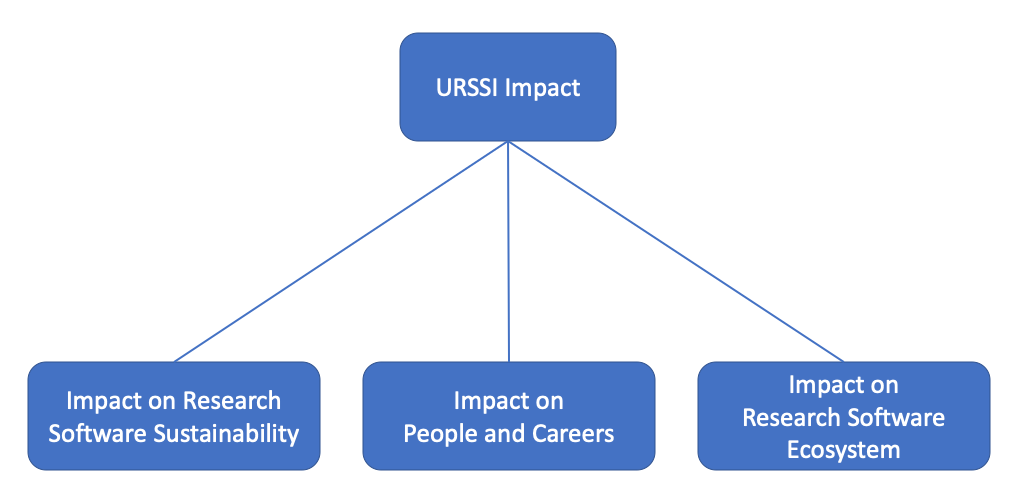
\includegraphics{images/URSSI-impact-drawing.png}

For software, URSSI aims to improve the sustainability of research software by

\begin{itemize}
\item
  Developing and curating best practices for software projects,
  including examining practices in industry,
  for testing, governance, codes of conduct, continuous integration.
\item
  Sharing information and practices through communities calls, training
  opportunities, an incubator, and a community-developed book
\end{itemize}

The activities that have a primary impact on the sustainability of research software are described in
\href{Ch-Comm}{Community \& outreach (Chapter 4)},
\href{Ch-Edu}{Education \& training (Chapter 5)}, and
\href{Ch-Incubator}{Incubator (Chapter 6)}.
Additionally, some activities in
\href{Ch-Policy}{Policy (Chapter 7)} have a secondary impact
on the sustainability of research software.

For people, URSSI aims to improve the careers of those who develop and maintain
research software by:

\begin{itemize}
\item
  Fellowships
\item
  In-person events and community calls
\item
  A summer school, and the incubator program
\item
  Promoting new career paths for those who develop and maintain research software
\item
  Developing and advocating for research software usage and impact metrics to be
  a factor in the hiring and promotion of software developers and maintainers,
  including promoting the publication of research software
\item
  Encouraging a diverse set of participants to enter the research software
  development and maintenance field and decreasing structural and systemic
  barriers to productive careers for members of underrepresented groups
\end{itemize}

The activities that have a primary impact on people and careers are described in
the four following chapters, on
\href{Ch-Comm}{Community \& outreach (Chapter 4)},
\href{Ch-Edu}{Education \& training (Chapter 5)},
\href{Ch-Incubator}{Incubator (Chapter 6)}, and
\href{Ch-Policy}{Policy (Chapter 7)}.

For the research software ecosystem, URSSI aims to improve the understanding and functioning of the ecosystem by

\begin{itemize}
\item
  In-person events and community calls
\item
  A newsletter and and an active social media presence
\item
  Incentivizing contributions to public software
\item
  Disentangling software quality and software impact, including
  promoting software credit and citation mechanisms
\item
  Documenting the use of research software in research and providing
  systematic and regular analysis of the impact this software has on research
\item
  Promoting an increased understanding of the importance of research software in research
\item
  Advocating for increased funding opportunities for software maintenance
\item
  Creating an award program to recognize software contributions
\item
  Growing and participating in communities around the field of research software
\end{itemize}

The activities that have a primary impact on the research software ecosystem are described in
\href{Ch-Comm}{Community \& outreach (Chapter 4)} and
\href{Ch-Policy}{Policy (Chapter 7)}.
Additionally, some activities in
\href{Ch-Edu}{Education \& training (Chapter 5)}
have a secondary impact
on the research software ecosystem.

\hypertarget{Ch-Comm}{%
\chapter{Community \& Outreach}\label{Ch-Comm}}

Researchers in academia and national labs are incentivized to become experts in one or more specialized domains.
While research software plays a critical role in achieving such mastery, skills to develop such software are rarely taught in formal settings.
These skills are often picked up from secondary special interest communities and online resources.
We plan to formalize such community resources and associated activities in our institute plans.

The institute's Community area will build a thriving community of like-minded peers for researchers to seek advice, learn about training opportunities, and funding announcements.
A community manager will curate state of the art information on best practices for research software development. We will work closely with The Center for Scientific Collaboration and Community Engagement (CSCCE) to train a research engineer who seeks to pursue a career in community management. CSCCE specalizes in professionalizing scientific community building and their training program can be completed while the community manager is getting started with their position.
The Community area will also administer a competitive fellowship program for early career researchers.
These fellowships will provide funding, training, and prestige/recognition to pursue a career that promotes the development and use of research software.
The thriving community will also provide venues and annual conference focused on software across disciplines where researchers can share their work, learn about new software, and software development techniques.

Many of the current challenges around sustainability of software, and those who produce it, are mostly social and cultural and not limited by any unassailable technical challenges.
While other areas of the institute such as Policy and Education \& Training lay down the guidelines and training necessary to grow the research software enterprise, a strong community strategy will be key to maintaining it.
URSSI will act as the hub for all types of researchers interested in using and developing research software.
The institute will provide necessary resources to address shared challenges and help catalyze collaborations to tackle emerging problems.
URSSI's Community \& Outreach area will achieve this mission through the set of activities described below.

\hypertarget{community-outreach-resources}{%
\section{Community \& Outreach Resources}\label{community-outreach-resources}}

Managing the URSSI community will require the following staff and resources:

\begin{itemize}
\item
  Managing communications (website with regular posts, moderating a mailing list), producing high quality newsletters, and acting as a community liaison will require 2-3 FTEs.
\item
  This could involve a Director of Community (could be part of a PI's time), with the remaining part of the area's workforce split over two positions: a community manager and fellowship coordinator (to be split with the Incubator Area), reporting to the Director of Community. We will work closely with The Center for Scientific Collaboration and Community Engagement to recruit one of their scientific community manager trainees as a fellow. We may also recruit someone who will undergo their training upon joining URSSI.
\end{itemize}

Besides the budget for the 2-3 positions, the Community \& Outreach area of the institute will also require budget for:

\begin{itemize}
\item
  Technical infrastructure (including: website, mailing list, archiving of resources). Maintaining a high quality newsletter will require access to high quality data feeds, all of which require paid subscriptions. The team will also require technical help to maintain a static site on GitHub.
\item
  One URSSI fellow (as part of a cohort of 4-5 fellows/year) can be asked to focus on community. Much like the BSSW fellowship, an URSSI fellow can propose a community related topic to pursue for the year of their fellowship.
\item
  Participant support for fellows and speakers to attend annual meetings
\item
  Base costs for an annual URSSI conference (with the rest to be supported by registration and sponsorships)
\end{itemize}

\hypertarget{community-outreach-methods}{%
\section{Community \& Outreach Methods}\label{community-outreach-methods}}

\hypertarget{fellowship-program}{%
\subsection{Fellowship Program}\label{fellowship-program}}

URSSI will run an annual fellowship program modeled heavily on the successful program run by the UK Software Sustainability Institute \citep{10.12688/f1000research.16231.1}. We will recruit 3-5 fellows from a pool of US graduate students, postdocs, and research software engineers.
Since research software suffers from a lack of diversity, the fellowship selection process committee will focus on providing opportunities for candidates from underrepresented groups. The community team will rely on existing research and tools on candidate selection to make decision making transparent and free from human biases as much as possible \citep{10.1371/journal.pone.0231939}.
One of the criteria used to select fellows will be a diversity statement that fellows will be required to submit, and \textasciitilde50\% of the selected fellows will be members of underrepresented groups, with a lower bound of 25\%.
Each fellow will affiliate with one or more areas of URSSI (Policy, Education, Community, Incubator) and propose an activity that would take no more than 1 day a week of their time. Fellowship stipend will provide an appropriate time buyout and also cover travel to \href{https://eng.ox.ac.uk/events/ssi-collaborations-workshop-2020/}{biannual collaborations workshops}, and the annual URSSI conference. Fellows will be given an additional travel budget to present their research software activities at society and discipline conferences. Each fellow will be paired with an URSSI mentor and success will be based on entry and exit interviews.

The fellowship program is aimed at the people and careers portion of URSSI's impact goals.

\hypertarget{in-person-events}{%
\subsection{In-person events}\label{in-person-events}}

Create new community events:
Building upon the work of small workshops such as Workshop on Sustainable Software for Science: Practice and Experiences (WSSSPE), there is an opportunity for URSSI to host an annual in-person conference for scientists, developers, and students to connect and discuss research software development and their applications.
One of the criteria used to select funded attendees will be a diversity statement that applicants will be required to submit, and at least 25\% of the selected applicants to be funded will be members of underrepresented groups.
The conference will initially be medium sized (with a limit of 300 participants) and grow depending on the interest.
Talks and workshops will span the entire continuum from applied computational research to software development.
The event will also feature a ``demo day'' for URSSI incubated projects, which would be a cross cutting activity with the Incubator program.
The costs for such an event will be supplemented by a mix of registration fees and sponsorships.

In-person events are aimed at the people and careers and research software ecosystem portions of URSSI's impact goals.

\hypertarget{online-community-events}{%
\subsection{Online community events}\label{online-community-events}}

Promote existing activities: One of URSSI's strengths will lie in amplifying the work of existing initiatives.
We will achieve this by showcasing projects in our weekly newsletter, by inviting projects to present their work on monthly community calls (aka webinars), and by highlighting/crossposting news via partner organizations such as the Carpentries, rOpenSci, Workshop on Sustainable Software for Science (WSSSPE), Mozilla, and others. The community manager will work with various parters and data feeds to curate and disseminate a high quality newsletter similar to the the data science newsletter operated by the Academic Data Science Allaince (ADSA). The institute will budget for costs associated with newsfeed subscriptions.

Community calls: Modeled after the successful series organized by Mozilla and rOpenSci, a monthly webinar series will expose researchers to the latest best practices and new trends in research software, and will provide them an opportunity to interact with prominent research software engineers.
This free and open series will provide additional opportunity for the community to participate, especially for those that are constrained by travel.
Past calls, including videos, code, and Q\&A will be archived and made searchable by a dedicated community coordinator.
We will consider diversity when chosing participants who will present in these calls, and seek to have at least 25\% of the presenters being members of underrepresented groups.

Online community events are aimed at all three portions of URSSI's impact goals: research software sustainability, people and careers, and the research software ecosystem.

\hypertarget{Ch-Comm-Best-Practices}{%
\subsection{Curating and disseminating best practices}\label{Ch-Comm-Best-Practices}}

URSSI fellows will convene ad hoc panels of experts to curate information on state of the art practices for scientific computing.
The topics will cover many foundations of research software engineering including but not limited to collaborative software developing with modern version control, software testing, code review, packaging and distribution, and overall software design.
The materials will also provide strong guidance on open science practices to increase impact of such work.
These include guidance on licensing, properly archiving research software, and citation.

Curating and disseminating best practices is primarily aimed at the research software sustainability portion of URSSI's impact goals, and secondarily at the people and careers and research software ecosystem portions.

\hypertarget{newsletter-and-social-media}{%
\subsection{Newsletter and social media}\label{newsletter-and-social-media}}

There is a huge opportunity for URSSI to produce and disseminate a high quality newsletter to keep the community informed about research software news, notable research papers, critical software, events and job openings.
The data science community already benefits from such \href{https://cds.nyu.edu/newsletter/}{a newsletter} that is maintained by Laura Noren and Brad Stegner and financially supported by the Academic Data Science Alliance.
The community manager will curate news, jobs, software releases, conferences, and activities of other organizations (by crossposting).
For community calls, we will invite speakers from related communities such as SSI, BSSw, US-RSE, and also solicit presentations from the larger community.
All material will be stored in public GitHub repositories under a permissive license to allow people to use and remix the content while contributing back to the original source.

The four major channels of communication will be a website, a newsletter, mailing list, and accounts on social media such as Twitter and Slack.

The newsletter and social media are primarily aimed at all the research software ecosystem portion of URSSI's impact goals, and secondarily at the research software sustainability and people and careers portions.

\hypertarget{other-activities}{%
\subsection{Other activities}\label{other-activities}}

Besides the activities described above, the institute will feature these ongoing activities:

\begin{itemize}
\tightlist
\item
  URSSI will serve as a broker for software expertise and connect developers to scientific projects seeking contractors, expert advice or collaborators on grants. The community team will coordinate some combination of a job/skills board to better leverage expertise among US institutions. {[}TODO: Flesh out details of this program{]}
\item
  Promote training events from URSSI and other communities
\item
  Develop an ambassador program for early career researchers to promote sustainable software and current issues to their local communities. Examples of similar programs include the \href{https://www.xsede.org/community-engagement/campus-champions}{Campus Champions program} at \href{https://www.xsede.org/}{XSEDE}, and the SSI fellows program \citep{10.12688/f1000research.16231.1}.
\end{itemize}

An URSSI ambassador program will be a light touch activity (less engaged than the fellows program) and provide students at US colleges and universities with resources to support campus colleagues effectively use research software to advance their research. The program will provide a venue to build community among early stage students (advanced undergraduates, beginning graduate students).
One of the criteria used to select ambassadors will be a diversity statement that potential ambassadors will be required to submit, and at least 25\% of the ambassadors will be members of underrepresented groups.

\begin{itemize}
\tightlist
\item
  Hosting a blog, with a series of staff and guest blog posts, including cross-posting relevant blog posts from others
\end{itemize}

\hypertarget{community-outreach-assessment-and-metrics}{%
\section{Community \& Outreach Assessment and Metrics}\label{community-outreach-assessment-and-metrics}}

\textbf{Goals: }

\begin{itemize}
\tightlist
\item
  Steadily grow the number of subscribers and participants each year
\item
  Grow the diversity of participants, instructors, and speakers each year. Self reported data on affiliations and domains of expertise will also provide a measurable metric of impact across domains.
\item
  Grow the number of applications we receive for the fellowship program every year
\item
  Grow the rate of paper and poster submissions every year
\item
  Improve the careers of those who participate in URSSI
\end{itemize}

\textbf{Metrics:}

\begin{itemize}
\tightlist
\item
  Number of subscribers to the newsletter, visitors to the website, and social media followers over time
\item
  Quantify instructors, presenters, lesson developers, and participants by demographic and geographic breakdown
\item
  Count citations of software that have participated in URSSI
\item
  Tracking career paths of fellows will also act as a measure of success for the program
\end{itemize}

\textbf{Impacts:}

This table maps URSSI activities from this chapter to the three portions of URSSI's intended impact.
(A complete table of impacts from all URSSI activities can be found in \href{Ch-Metrics}{Chapter 10 (Metrics and Evaluation)}.)
In the impact cells, X indicates a designed primary impact on an activity, and y indicates
a designed secondary impact.

\begin{table}

\caption{\label{tab:unnamed-chunk-1}Impact table}
\centering
\begin{tabular}[t]{lccc}
\toprule
Activity & Impact on Research Software & Impact on people and careers & Impact on research software ecosystem\\
\midrule
Fellowships &  & X & \\
In-person events &  & X & X\\
Community calls & X & X & X\\
Curate best practices & X & y & y\\
Newsletter \& social media &  & y & X\\
\bottomrule
\end{tabular}
\end{table}

\hypertarget{Ch-Edu}{%
\chapter{Education \& Training}\label{Ch-Edu}}

Researchers often view software development skills as separate from, but complementary to
their disciplinary training. This perspective introduces a dilemma for researchers, particularly
for early-career researchers, who need to master their discipline and simultaneously acquire
sufficiently-good software engineering skills. When forced to choose, they typically make sacrifices
or take shortcuts in software engineering, as they view their disciplinary skills and knowledge as
more important to their careers, and more rewarded by current incentive systems. Further, many
researchers do not aspire to become software engineering experts, but approach the acquisition of
software skills as a means to a research end. This approach is implicitly encouraged by the fact
that the educational content of most disciplines that require software skills does not actually
include sufficient discussion of software development or engineering. As a result, there are valuable
skills such as packaging, testing, releasing, archiving, and even designing research software that
are dramatically underdeveloped in the overall research ecosystem.

Indeed, previous studies demonstrate that researchers are rarely purposely trained to develop software.
A 2017 survey of US National Postdoctoral Association members regarding postdocs' use of software in
research and their training regarding software development found that 95\% of respondents use research
software. However, 54\% (n = 104) of the respondents to this survey reported that they have not
received any training in software development \citep{nangia_katz_2017}. A similar survey of software
use and training from the UK repeats this finding: in 2014, Hettrick et al.~asked researchers at
randomly selected researchers at 15 Russell Group universities about their software use and training.
Of the 417 responses, 45\% reported having no training in software development. Of the 55\% of respondents
that reported having received training in software development, 73\% had received some form of
formal training in a software development course, the remaining 27\% were self-taught. In further analyzing
these results, Hettrick et al.~report that 21\% of respondents who develop their own software had
no training in software development \citep{simon_hettrick_2018_1183562, Hettrick-blog}. A 2016 survey
of 704 PIs from the Biological Sciences Directorate of the US NSF found the most pressing unmet
needs are training in data integration, data management, and scaling analyses for HPC \citep{barone2017unmet}.
And a 2018 survey of almost 1600 scientist-developers found that 82\% of respondents felt that
they were spending ``more time'' or ``much more time'' developing software than they did 10 years ago \citep{Pinto2018}.

Not only is there a gap in software development training in general, there's also an additional
gap across gender. When analyzed by gender (self reported binary of men and women) the first
two surveys show that only 39\% of female respondents in the UK and 32\% in the USA report
have received some form of software development training, compared to 63\% of male respondents
in the UK and 64\% in the USA.

This lack of training is not new, nor is it newly discovered. Greg Wilson has written
\citep{wilsong2016, softwarecarpentryhistory} about the history of Software Carpentry:

\begin{quote}
In 1995--96, {[}Wilson{]} organized a series of articles in IEEE Computational Science \&
Engineering titled, ``What Should Computer Scientists Teach to Physical Scientists and
Engineers?''. These grew out of the frustration he had working with scientists who wanted
to run before they could walk, i.e., to parallelize complex programs that were not broken
down into self-contained functions, that did not have any automated tests, and that were
not under version control.
\end{quote}

\begin{quote}
In response, John Reynders (then director of the Advanced Computing Laboratory at
Los Alamos National Laboratory) invited {[}Wilson{]} and Brent Gorda (now at Intel) to
teach a week-long course to LANL staff. This course ran for the first time in July
1998, and was repeated nine times over the next four years. It eventually wound down
as Gorda and {[}Wilson{]} moved on to other projects, but two valuable lessons were learned:

\begin{enumerate}
\def\labelenumi{\arabic{enumi}.}
\item
  There is tremendous pent-up demand for training in basic skills.
\item
  Textbook software engineering is not the right thing to teach most scientists.
\end{enumerate}
\end{quote}

This need led to the Software Carpentry organization, which built a successful train-the-trainer
model for collaborative lesson development and delivery, and which was used as a model
to build Data Carpentry, which then merged with Software Carpentry into The Carpentries,
and now also includes Library Carpentry. The Carpentries has developed highly impactful
training content and events that meet an intermediate need for training researchers to
better develop software. Many computing centers, including those funded by NSF and DOE,
have also long had user training in some types of development (similar to that of Los
Alamos), for example, joint activities run by
\href{https://www.xsede.org/wwwteragrid/archive/web/eot/workshops.html}{TeraGrid} and now
\href{https://www.xsede.org/for-users/training}{XSEDE}, and Argonne's
\href{https://extremecomputingtraining.anl.gov}{ATPESC}. Given the success of the Carpentries,
these computing center training events often either include or contribute to Carpentries
lessons, or complement them. In addition, other NSF-funded software institutes (e.g.,
MolSSI, SGCI, and IRIS-HEP) are also developing training resources for their target
communities, similarly making use of, contributing to, and complementing the Carpentries.

While many researchers may learn how to program on their own, the opportunities for them
to learn software engineering and software deisgn are less available. Therefore, we believe
that there is an important role that a US-based research software institute
can play to expand the breadth and depth of the training available, and to further
coordinate and facilitate the acquisition of software engineering expertise by researchers
engaged in various development activities. Rather than reinventing content, we anticipate
collaborating with and pointing to relevant resources developed through other related efforts.

The Education \& Training thrust of URSSI complements and builds upon existing efforts through
the following planned activities (more detail appears below):

\begin{enumerate}
\def\labelenumi{\arabic{enumi}.}
\item
  Develop and annually run a summer school on practices for sustainable software development
  for research software.
\item
  Develop a Research Project Carpentry lesson program that teaches people how to turn code
  into a formal project.
\item
  Plan a review service for software project plans (and note that the implementation of this
  plan is likely out of scope of URSSI by itself).
\item
  Evaluate and document successes and failures of industrial software development practices
  in research software.
\item
  Compile and maintain a body of knowledge of best practices for research software development.
  (This URSSI activity will seek to aggregate both existing practices, and serve as an outlet
  for emerging practices from other domain-specific software institute, e.g., MolSSI, SGCI, IRIS-HEP)
\end{enumerate}

\hypertarget{education-training-resources}{%
\section{Education \& Training resources}\label{education-training-resources}}

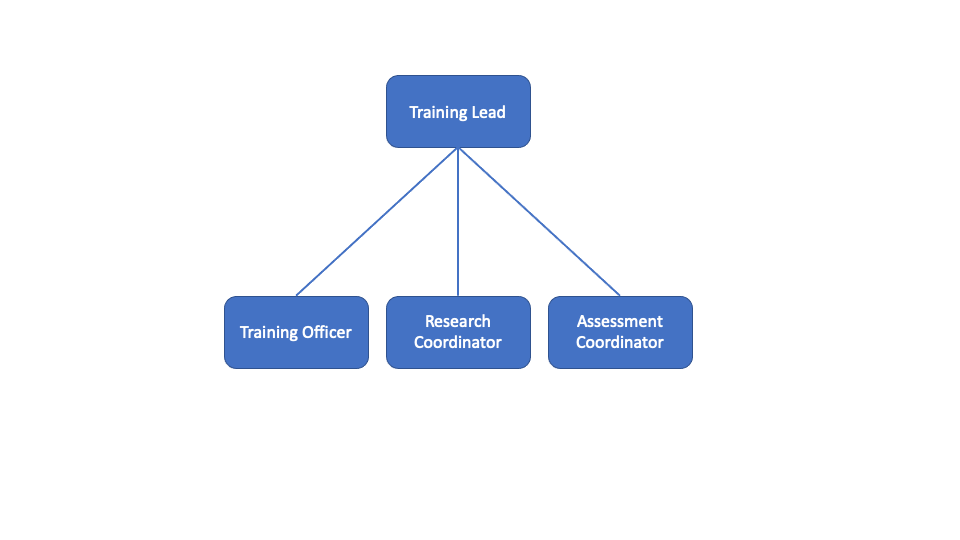
\includegraphics{images/education_structure.png}

This area requires the following staff:

\begin{itemize}
\item
  Training Lead: coordinates all training activities and assessment of those
  activities (1 FTE).
\item
  Training Officer: assists Training Lead in coordination of training activities,
  develops and delivers training activities (1 FTE).
\item
  Assessment Coordinator: leads the assessment efforts, in conjunction with the Training
  Lead (this position could be shared with other parts of the project) (0.5 FTE).
\item
  Research Coordinator: leads the effort to gather experiences from research
  software projects (0.25-0.5 FTE).
\end{itemize}

\hypertarget{education-training-methods}{%
\section{Education \& Training methods}\label{education-training-methods}}

This section provides more details on how we plan to design and execute each of these
activities within URSSI.

\hypertarget{develop-and-annually-run-a-summer-school-on-practices-for-sustainable-software-development-for-research-software}{%
\subsection{Develop and annually run a summer school on practices for sustainable software development for research software}\label{develop-and-annually-run-a-summer-school-on-practices-for-sustainable-software-development-for-research-software}}

\emph{Overview}: During the conceptualization phase, we identified a need for additional,
focused training opportunities on sustainable software development practices for researchers
who were not in a domain covered by an existing institute. One of the primary reasons for
this need is that it is generally difficult for degree programs to make room for this type of
content. We plan to meet this need with a summer school, which is a proven method for
providing hands-on training to transfer these skills to students, in this case on sustainable
software development practices for research software development. We conducted a Pilot
Winter School as part of the conceptualization process. The details of that activity appear
in \protect\hyperlink{chapter2-WinterSchool}{Chapter 2}. The plan described here builds on the key lessons
learned, including: (1) the school needs to be longer to allow for both discussion time
and focused time for students to work on their own code, applying the lessons from the
lectures, and (2) the presence of additional helpers outside of the primary instructors
was quite beneficial to help answer specific questions from the students.

\emph{Content}: Based on the needs identified during our survey, workshops, and other discussions,
we identified the following topics as candidates for inclusion in such a school:
(1) software design (including modularity), (2) software testing,
(3) packaging and distributing code,
(4) collaborative software development with modern version control (i.e., git/GitHub),
(5) peer code review, (6) open science principles, and (7) software citation.

\emph{Format}: The summer school will be a 1-week in-person event. We plan to follow the
successful PNAS hackweek model \citep{Huppenkothen8872} where we allocate 50\% of the time
to lectures and 50\% of the time to putting the concepts into practice. We will
invite instructors with expertise in the different topic areas (see above) to participate
and deliver the lectures, and will take diversity into consideration when selecting instructors.
One of the criteria used to select participants will be a diversity statement that potential participants
will be required to submit, and at least 25\% of the selected participants will be members of underrepresented groups.
To facilitate the ``hacking'' time,
we will ask participants to bring a code project they wish to work on during the
school. The ``hacking sessions'' will provide ample opportunities for the participants to
have hands-on time applying the concepts from the lectures to their own code projects. These sessions
also provide time for code reviews and other ad hoc topics that arise during the school.
The instructors will be available during the hands-on time to help participants as
needed. By the end of the school, participants should have substantial intellectual
knowledge and experiential knowledge. Because researchers often do not have sufficient
time for training or to attend events like this one, as an alternative to the face-to-face
summer school events, we also plan to package the content into Carpentries-style lessons
that can be used either in shorter training sessions, webinars, or asynchronously.

The URSSI summer school is primarily aimed at the people and careers portion of URSSI's impact goals, and secondarily at the research software sustainability and research software ecosystem portions.

\hypertarget{develop-a-research-project-carpentry-lesson-program-that-teaches-people-how-to-turn-code-into-a-formal-project}{%
\subsection{Develop a Research Project Carpentry lesson program that teaches people how to turn code into a formal project}\label{develop-a-research-project-carpentry-lesson-program-that-teaches-people-how-to-turn-code-into-a-formal-project}}

\emph{Overview}: One challenge faced by many research software developers is how to convert
a small (individual) coding effort into a more formal project. This situation occurs
frequently as researchers develop small units of code to accomplish tasks important in
their own work. When other researchers are exposed to these code units, they often want
either to use the code, add to the code, or both. This is the point when the researcher
needs to convert that code into a more formal project, both to ensure quality as others
use it and to allow the community to contribute to it. Therefore, we propose to develop
a Research Project Carpentry lesson plan, along similar lines as Software Carpentry, that
will help researchers make this transition from an individual coding effort to a
community-focused project.

\emph{Content}: The goal of this effort will be to help projects develop a good project plan.
As such, the Research Project Carpentries lesson program will focus on helping researchers
understand what content a good plan needs to contain. It will also provide information
researchers need for making choices about which of the various practices are most relevant
to their particular project. The topics to be covered in Research Project Carpentry include:
(1) requirements elicitation, (2) issue tracking, (3) source and version control, (4) testing,
(5) documentation, (6) packaging and distribution, (7) pair programming, (8) code review, and
(9) metrics. Note that there is some overlap between the focus of Research Project Carpentry
and the Summer School described above. We anticipate reusing relevant content between these efforts.

\emph{Format}: We will develop modules on the topics above as carpentries-style modules. This approach
will allow the Research Projects Carpentries materials to be used either in a face-to-face training
course, like the Summer School, or as stand-alone units. This flexibility will allow researchers
to access the content in a mechanism that is most relevant to them. When this material is tested,
we will use use a diversity statement submitted by potential participants as an input to the decision
process, and at least 25\% of the selected participants will be members of underrepresented groups.

\emph{Note}: While this activity is relevant to the URSSI effort, we believe that it will have appeal
beyond URSSI. Therefore, even though we include it here in the plan, we will also seek funding to
support it from organizations outside of NSF. We also plan to solicit other organizations and
individuals to contribute to this activity. URSSI will lead this work, organizing a community
that will include external participants.

The Research Project Carpentry lesson program is primarily aimed at the research software sustainability portion of URSSI's impact goals, and secondarily at the research software ecosystem portion.

\hypertarget{plan-a-review-service-for-software-project-plans}{%
\subsection{Plan a review service for software project plans}\label{plan-a-review-service-for-software-project-plans}}

Building on the work done for Research Project Carpentries, URSSI has identified the need for
a service where experts review and comment on proposed project plans. Researchers who are
interested in this service would submit a project plan in a specified format. Then, experts
would review the plan to ensure both that it is (1) complete with respect to the content necessary
for the type of project and its current stage, as well as (2) the choices made for each aspect of
the project plan are consistent with best practices. Once the review is completed, the reviewer
would work with the project team to help resolve any deficiencies identified in the original
project plan. This model is akin to that used by many ``incubators'' for start-up companies.

This activity is likely beyond the scope of URSSI, so we will create an initial plan for it,
then seek to partner with other organizations who are pursuing similar efforts and explore
external funding sources. In addition to the operating the service, URSSI and partners will need
to develop and make available the following resources: (1) templates for project plans,
(2) checklists for researchers to follow when developing the plan, and (3) guidance on how
to choose from various alternatives for each section of the plan.

The softare project plan review service is aimed at the research software sustainability portion of URSSI's impact goals.

\hypertarget{evaluate-and-document-successes-and-failures-of-the-use-of-industrial-software-development-practices-in-research-software}{%
\subsection{Evaluate and document successes and failures of the use of industrial software development practices in research software}\label{evaluate-and-document-successes-and-failures-of-the-use-of-industrial-software-development-practices-in-research-software}}

Industrial software engineering has developed and refined a number of best practices for
software engineering and software development, resulting in a large body of related literature.
Conversely, it is not always clear which of these practices are relevant for use in developing
research software, most notably because of the different incentive structures for developers
in the research arena. It is also not always clear which aspects
of the research software domain motivate the need to develop new software engineering or
software development practices to handle the unique contexts within which research software
exists. To accomplish this activity, URSSI will need to perform the following steps.

First, URSSI will gather experience reports describing the successful and unsuccessful use
of industrial software engineering and software development practices in research software
projects. Gathering these experiences will involve conducting surveys and interviews of
developers of research software to document important information. In addition to the
successes and failures with specific practices, these experience reports will also document
cases where developers of research software encountered a situation or a problem for which
they were unable to find software engineering or software development practices that were
relevant. Cases where there is a lack of relevant practices suggest opportunities for
creation of new practices.

Second, URSSI will analyze the experience reports to systematize the successes and failures
and develop a series of evidence-based lessons learned. Because this information will be
based upon real experiences from research projects, they will have great value to other
research software projects.

The results of these efforts will feed into the next activity by providing concrete experiences
that we can document into best practices. These experiences will be beneficial because we
will draw them from experiences on real projects, with knowledge about the context within
which the practice works. This context will help provide a description of the limitations
on the practice, which is equally important to document.

This activity is primarily aimed at the research software sustainability portion of URSSI's impact goals, and secondarily at the research software ecosystem portion.

\hypertarget{compile-and-maintain-a-body-of-knowledge-of-best-practices-for-research-software-development}{%
\subsection{Compile and maintain a body of knowledge of best practices for research software development}\label{compile-and-maintain-a-body-of-knowledge-of-best-practices-for-research-software-development}}

Based on the outcomes of the above activities, URSSI will develop a portal to provide living
information about best practices for research software development. In addition to including
content developed from our own activities, URSSI will also actively find, through various
means that include workshops and surveys, and curate information from other sites related
to the development of research or scientific software. We will specifically ensure that
information produced by the Carpentries is included, as relevant.

We will curate the following types of information:

\begin{enumerate}
\def\labelenumi{\arabic{enumi}.}
\item
  Checklists for sustainable software - much of the content here will overlap with
  ideas discussed in earlier activities.
\item
  Templates for use in developing software, including templates for project plans,
  templates for documenting requirements, templates for test planning, and templates
  for community guidelines and policies.
\item
  Badging efforts that provide recognition for various qualities of research software
  and research software projects.
\end{enumerate}

In addition to best practices, the URSSI clearinghouse will also curate information
about training resources. In addition to providing links to the URSSI-developed training
(described above), we will also link to other relevant training resources developed
through other efforts like MoLSSI, SGCI, and IRIS-HEP. To help individual researchers
and teams better understand how to make use of the various training options, we will
develop roadmaps that guide people to the most relevant training for their current situation.

This activity is also primarily aimed at the research software sustainability portion of URSSI's impact goals, and secondarily at the research software ecosystem portion.

\hypertarget{cross-cutting-activities}{%
\section{Cross-cutting activities}\label{cross-cutting-activities}}

To support the five activities described above, URSSI will also need to perform a number
of cross-cutting activities as follows:

\begin{enumerate}
\def\labelenumi{\arabic{enumi}.}
\item
  \emph{Curriculum Development and Coordination}
  To achieve the goals stated above, URSSI will need to support the development of new
  training materials. We anticipate providing support to experts in the research software
  community who can take their existing knowledge and package it in a Carpentries-style
  format that is most amenable to be used in the various types of training activities URSSI
  will support. Importantly, the training proposed above is meant to build upon, and
  provide a complement to existing educational outreach efforts. This training will provide
  follow on, more advanced content than the Carpentries, and will be longer in duration.
  We can provide this advanced content because our target audience is a subset of the audience
  focused on by the Carpentries.
\item
  \emph{Instructor Training}
  To help deliver all of the developed content to a wide range of audiences in various
  locations, URSSI will need to provide support for training instructors. These instructors
  will be integral to the success of the Summer School and the Research Projects Carpentry.
\item
  \emph{Piloting Workshops}
  As we develop content, we will conduct smaller workshops to pilot the content to ensure
  its sufficiency before deploying it to a larger audience. Because we will be asking people
  to participate in content development by providing feedback, we will need to have resources
  to support the travel for instructors and participants.
\item
  \emph{Gathering Experiences on Successes and Failures of Software Practices}
  URSSI will support a team of researchers, who are experienced in survey and interview methods,
  to gather experiences, summarize the results, and document the findings. In addition, URSSI will
  need to provide support for travel for URSSI personnel to meet with members of research projects.
\item
  \emph{Conducting Workshops}
  URSSI will provide support for the Summer School and Research Project Carpentries instructors
  to travel to the workshops. URSSI will also provide small fellowships for the instructors
  to compensate for the time required to participate. In addition, to increase participation
  from a diverse community, URSSI will provide travel support for a small number of workshop
  participants, determined based on need in individual cases.
\item
  \emph{Packaging and Sharing}
  As URSSI develops content related to the educational activities described in this chapter, we
  will package that content in a shareable format. We will make the content freely
  available on GitHub. We will also archive each release of content on Zenodo using a proper
  license that allows anyone to use and/or modify the content as needed. In addition, we will
  strive to work with the Carpentries to enable the content to reach more people.
\end{enumerate}

\hypertarget{education-training-metricsmilestones}{%
\section{Education \& Training metrics/milestones}\label{education-training-metricsmilestones}}

To ensure that the training activities are providing sufficient content, URSSI will conduct
numerous assessment activities. These activities will occur both concurrently with the
training activities, i.e., as entry and exit surveys, as well as longitudinally after
training. The benefit of conducting assessment longitudinally is that it provides insight
into whether the content learned during training is viewed as useful over time as real
projects evolve.

Some of the specific measures that we will gather include:

\begin{itemize}
\item
  Post-event evaluations: For workshops and training courses, we will conduct follow-up surveys
  to evaluate the value of the content. We will conduct evaluations immediately at the end of
  each event while the information is fresh in the attendees' minds. We will then conduct a
  follow-up survey 6 months, 1 year, and 3 years later to evaluate the applicability of the
  content to the attendees' work. In conducting these evaluations, we will build on lessons
  learned and guidance from \href{https://carpentries.org/assessment-network/}{The Carpentries Assessment Network}.
\item
  Demand: We will measure demand for the content by the number of people who apply to attend
  various training events and workshops.
\item
  Use of material: We will measure downloads and use of the information that we produce.
\end{itemize}

\textbf{Impacts:}

This table maps URSSI activities from this chapter to the three portions of URSSI's intended impact.
(A complete table of impacts from all URSSI activities can be found in \href{Ch-Metrics}{Chapter 10 (Metrics and Evaluation)}.)
In the impact cells, X indicates a designed primary impact on an activity, and y indicates
a designed secondary impact.

\begin{table}

\caption{\label{tab:unnamed-chunk-2}Impact table}
\centering
\begin{tabular}[t]{lccc}
\toprule
Activity & Impact on Research Software & Impact on people and careers & Impact on research software ecosystem\\
\midrule
Summer school & y & X & y\\
Projects Carpentry & X &  & y\\
Review service for software project plans & X &  & \\
Examine use of industrial software development practices in research software & X &  & y\\
Book of knowledge of software dev best practices & X &  & y\\
\bottomrule
\end{tabular}
\end{table}

\hypertarget{Ch-Incubator}{%
\chapter{Incubator}\label{Ch-Incubator}}

The intent of an URSSI Incubator is to support software projects seeking to grow, transition to an open-source model of development, or improve software engineering practices. The incubator plans to do this by providing mentorship, a small amount of funding, and guided support for improving governance, documentation, financial planning, and evaluating development practices. The following sections describe the motivation for an Incubator program focused on research software.

\hypertarget{background}{%
\section{Background}\label{background}}

Common tasks solved by research software often include the generation, analysis, visualization, and processing of data.
These software solutions are, just as often, generalizable beyond the immediate needs of an individual researcher, research group, or a particular research effort. However, there are few institutional and personal incentives to develop generalizable research software, package this software for reuse, create meaningful documentation, and share software in open repositories.
Each of these activities requires substantial investments of time, money, and effort.

For researchers the return on this investment may be minimal - software is rarely cited in scholarly literature \citep{howison2016software, hwang2017software, hsu2019comparing, park2019research}, tenure and promotion committees rarely consider software contributions \citep{moher2018assessing}, and grant funding often acknowledges software development as a byproduct of rather than a substantive contribution to a research project \citep{broman2017recommendations, siepel2019challenges}.

These challenges are despite increasing evidence of the value of software sharing and reuse in addressing research challenges that require fast and efficient community response.
For example, the Medical Research Center in the UK is currently using a 13 year old pandemic simulation codebase to model control measures for COVID-19.
In doing so, they've attracted collaborators from Microsoft, the Abdul Latif Jameel Institute for Disease and Emergency Analytics, and the WHO Collaborating Centre for Infectious Disease Modelling to document, refactor, and extend this code.
While the original author of the simulation code acknowledged its numerous imperfections \footnote{See \href{https://twitter.com/neil_ferguson/status/1241835454707699713}{Neil Furguson's tweet} for an extended commentary}, the ability to start from an existing working model saved time, money, and effort in combating a global pandemic.

Contemporary research is littered with similar examples - imperfect software that is valuable for one purpose can be made more broadly useful by being shared, properly documented, and made available for sustainable reuse.
Finding ways to encourage and support research software so that it remains accessible for future improvements and uses is a primary goal of URSSI.
But, there currently exists little guidance for how a single research software project can transition from the individual efforts of a small set of researchers to a distributed open model of development that attracts and retains valuable communities of contributors \citep{howison2015sustaining}.

Open source models are a helpful, but not the only, reference for the forms of cooperative community organizing that we believe will be valuable to developing a more sustainable research software ecosystem.
An open-source model has some basic features for community development that are necessary for sustainable research software: code is openly licensed for reuse, members are distributed across time and space, and the organization of development efforts depend, in part, upon loosely connected individuals making small contributions (or peer-production) \footnote{ See the Open Source guide on \href{https://opensource.guide/building-community/}{building community}}.
These types of models for collaboratively organizing a software project are substantially different from how most researchers are trained and learn to develop software.
Most research software development is currently focused on solving immediate short-term individual needs rather than collaboratively building generalizable solutions or performing necessary maintenance of this software \footnote{Rene Gassmoeller has made this argument succintly in a recent \href{http://urssi.us/blog/2020/03/24/scientific-software-projects-and-their-communities/}{blog post}}.
These are obviously beneficial and valuable modes of collaborative software development that can and should play a more prominent role in the research software ecosystem.
In the following section we further justify some of our working assumptions about why open models of software development can lead to more sustainable research software, and then propose the design and implementation of a research software incubator program that would help foster a transition to open-source, or similar, forms of research software development.

\hypertarget{evidence-base}{%
\section{Evidence base}\label{evidence-base}}

There currently exist several detailed taxonomies of successful open source community models, including the \href{http://community.apache.org/apache-way/apache-project-maturity-model.html}{Apache Project Maturity Model} and Mozilla's \href{https://blog.mozilla.org/wp-content/uploads/2018/05/MZOTS_OS_Archetypes_report_ext_scr.pdf}{Open Source Archetypes}.
The features that differentiate one open source model from another are often subtle, but important, in project organization, credit distribution, and methods for reaching consensus on strategic decisions. Decades of empirical research into open-source provides the following key findings relevant for the likely success of distributed research software development:

\begin{itemize}
\item
  \textbf{Governance} in open source often includes a framework for organizing distributed work, establishing formal and informal roles for participants, managing access to resources, and distributing credit for work performed \citep[ ]{o2007governance}.
  Many previous studies of open-source success (measured as the long-term usefulness or accessibility of a codebase) have shown that vertical authority structures (such as how decisions are made and responsibilities are delegated) and horizontal coordination (open contributions) are key governance features that frameworks can help to make explicit and transparent \citep{stewart2016studies}.
  As contributors and maintenance responsibilities grow in scope, software governance research has also emphasized the importance of designing coordination processes so that contributors can be empowered to self-select tasks that lead to positive outcomes for a software project over time \citep{shaikh2017governing}.
\item
  \textbf{Documentation} plays a key role in open-source projects - it eases the onboarding of new contributors and plays an important role in the effective reuse or repurposing of a software package \citep{aversano2017evaluating}.
  Documentation is also an important, but often underdeveloped, aspect of software development in research settings \citep{geiger2018types}.
  Underdeveloped documentation is true of all software development \footnote{In GitHub's annual developers survey documentation was noted as the biggest barrier to engaging with open-source software \url{https://opensourcesurvey.org/2017/}}, but the tedious and time consuming tasks related to creating useful documentation are arguably more difficult in research settings where the development activities focus on solving practical problems in analyzing or interpreting data \citep{ram2018community}.
\item
  \textbf{Maintenance} is also a key element of open-source development activities.
  Maintenance includes solving problems introduced by operating system changes, code defects, and evolving software to meet emerging user requirements \citep{bourque2004swebok}.
  Open-source projects often face practical challenges in attracting and retaining maintainers.
  Previous empirical studies show that many projects on GitHub, for example, have only 1 maintainer \citep{eghbal2016roads}.
  Recent surveys of developers report that up to 86\% of projects have no maintainer \citep{coelho2017modern}.
\item
  \textbf{Licensing} is a key feature defining an open-source model of software development.
  But, developers often have a difficult time making licensing decisions without consultation of legal experts.
  A recent survey makes this point clear - up to 38\% (n=375) of experienced developers were not able to select an appropriate license given a scenario in which they were asked to identify an appropriate license for a given software library \citep{almeida2017software}.
  Developers' understanding of how to interpret licensing restrictions also significantly decreased in scenarios where multiple licenses were required.
\end{itemize}

For software projects that have the potential to broadly impact research communities, we believe that, at minimum, there should be greater support for making decisions about governance and licensing, and assistance in creating useful documentation that can attract new contributors or ease maintenance tasks.
Rather than simply creating a guidebook or articulating best practices for adopting open-source models of software development, a meaningful intervention for URSSI could include close interaction with and service to research software development projects that seek a route towards sustainability through community engagement and collaboration.

\hypertarget{incubators-background}{%
\section{Incubators background}\label{incubators-background}}

Incubators or business accelerators are a common way for venture capitalists to support entrepreneurs and ``start-up'' companies attempting to break into a new market.
These types of incubator programs often provide mentorship as well as fiscal support for a founder or product owner to identify market fit, build out or expand software features, and develop a network of interested stakeholders.
Successful graduation or exit from a start-up incubator is viewed as securing funding or launching a new product (often with a culminating event where the founder / product owner ``pitches'' the product to potential investors).
Successful start-up incubators like \href{http://www.techstars.com/}{Tech stars} or \href{https://www.ycombinator.com/}{Y Combinator} have designed processes for attracting, evaluating, and helping promising software-based projects achieve financial success. Y combinator for example has successfully graduated over 2000 companies that collectively have a market valuation over \$155 billion.

Open source incubators are less common. Perhaps the most successful and long running open-source incubator is by the \href{https://incubator.apache.org/}{Apache Software Foundation}, which provides a well documented process for software projects wishing to become part of the Apache Foundation \citep{schweik2012internet}.
Similar to a start-up incubator, the Apache model of incubation includes a project mentor and dedicated resources (infrastructure) for projects to develop releases of their software that comply with the Apache Foundation's standards.
Success, or graduation, in the Apache incubator is thus dependent upon making two consecutive software releases that are evaluated, and ultimately accepted by Apache developers.

Through conceptualization activities, notably community workshops, we began to formulate a plan for \emph{incubating} research software projects that would focus specifically on providing project developers time and support to improve the sustainability of their software projects.
A research software incubator would help projects identify and make strategic decisions about governance, assist research projects in creating valuable documentation, and strategically plan for transitions from individual or small teams to fostering a community of contributors and maintainers.

We believe that a research software incubator should have features similar to start-up and existing open-source incubators, but also should differ in appreciable ways.

First, we do not intend successful graduation or exit to be based solely on funding or code acceptance into a particular foundation structure.
Start-up incubators in particular focus on software development as a means to a company being acquired or receiving a large investment for future development.
Instead of focusing solely on growth for funding, we see a research software incubator model as providing the necessary time, mentorship, and financial support that will help a promising software project make decisions about how to improve the sustainability of their software and their project organization.
Second, and importantly, start-up incubators often provide financial support for founders to dedicate all of their time and attention to a project's successful graduation. This level of financial support is likely infeasible for URSSI.

Additionally, most researchers would have a very difficult time in dropping all other responsibilities at their institution to focus solely on a single software project that doesn't have the potential for a significant financial return on their investment of time and effort.
Therefore, we believe it is important to design a research software sustainability incubator in which a researcher can complete it with a small amount of effort and mentorship from the URSSI community.
We do not not expect that URSSI Incubator activities can or should be a project team's only focus.

\hypertarget{urssi-incubator}{%
\section{URSSI Incubator}\label{urssi-incubator}}

Our plan addresses problems related to credit, reward, and acknowledgement of research software development activities in its Policy area.
The URSSI Incubator proposal aims to provide multiple alternative pathways to sustainability through mentorship, project development advice or guidance, and strategic planning for governance.
We seek to help projects that show promise in solving general research problems mature, both the code and the project itself, in ways that are valuable to a broad community of potential users.
In doing so, we believe there is an opportunity to increase the sustainability of research software.

The broad goals of the URSSI Incubator program are:

\begin{enumerate}
\def\labelenumi{\arabic{enumi}.}
\item
  Provide the social and technical infrastructure to help research software projects become more sustainable.
  For projects that are growing, support will focus on how to achieve this growth in manageable ways.
  For projects that are already at a community level of contribution and development, support will help to identify and eliminate technical debt.
\item
  Provide research software projects, at various points in the development lifecycle, the opportunity to improve their development and organizational practices so as to mature, or develop, in ways that are broadly valuable to scholarship.
\item
  Provide an alternative to academic technology transfer offices. We believe there is an emerging need for guidance to scholarly research software projects that us focused not on commercialization but on a transition to open-source community models.
  Technology transfer programs at universities and through research funding agencies (e.g.~I-Corps, SBIR/STTR) are well established and have been successful at helping entrepreneurially-focused software projects recognize and execute viable business models. More recent examples of this model have focused on transition pathways towards openness, with a particular focus on open-source (e.g.~the \href{https://www.rit.edu/research/open}{Open@RIT} program at Rochester Institute of Technology)
  The commercial transition pathway is promoted for software that has the potential to sustain itself through fees or licensing agreements.
  However, there are currently few equivalent university guidance for software projects that would like to pursue non-commercial open source models for sustainability.
\item
  Provide guidance and mentorship in best practices for development, licensing, project coordination, and advice for funding to projects wishing to grow into community software projects.
  This component of the Incubator will draw upon expertise and guidance that is developed in URSSI's Education and Policy areas.
\end{enumerate}

\hypertarget{incubator-resources}{%
\section{Incubator resources}\label{incubator-resources}}

Personnel

\begin{itemize}
\tightlist
\item
  0.5 FTE Program Director shared with Education + Teaching, Policy, or Communications
\item
  1 FTE Program Lead. This individual would be in charge of coordinating the application and selection process, administering incubated projects, tracking success, coordinating an Incubator Advisory Board (described in detail below), and acting as the URSSI Incubator project manager.
\item
  Advisory Board (Volunteers). A group of senior researchers and software engineers who can offer strategic guidance to the Incubator program for meeting targeted goals.
\item
  Project Mentors (Volunteers + Graduated projects). Provide intensive, one on one mentoring to research software projects based on existing expertise in a discipline, software language, stage of development, or other criteria of compatibility.
\end{itemize}

Additional Resources that may be valuable for an incubator program to succeed:

\begin{itemize}
\tightlist
\item
  Annual Incubator showcase, or a ``demo day'', for projects that have successfully graduated or exited the URSSI's program. This activity could be part of a larger URSSI annual event that coordinates the community dedicated to software sustainability. Invitations to this event would be extended to public and private funders who may see an overlap with their own programs during pitches. This can result in matchmaking between projects and funders.
\item
  Incubated project funding: Monetary (or in-kind service) award for projects that will be given a budget to advance goals during a period of ``incubation''. Each project should receive a similar allocation of money. This money would be similar to how the SSI currently funds research fellows at a standard rate across their period of engagement. The money could be discretionary to the project so that it could be used for travel, advocacy, website development, assistance in writing documentation, etc.
\end{itemize}

\hypertarget{incubator-methods}{%
\section{Incubator methods}\label{incubator-methods}}

URSSI's Incubator program will include a process for soliciting applications (or call for participation), selecting participants, a cycle of activities, and a standard for successfully exiting or graduating from the Incubator.
The incubator will run on a semi-annual schedule so that new project cohorts can enter the Incubator in either January or July of each year.
In the following subsections we describe the intended processes for running each stage of the Incubator.

We view the Incubator as a single activity from the point-of-view of impact, and it is aimed at both the research software sustainability and people and careers portions of URSSI's impact goals.

\hypertarget{project-solicitation-and-selection}{%
\subsection{Project solicitation and selection:}\label{project-solicitation-and-selection}}

The URSSI Incubator will solicit proposals for projects three months in advance of the formation of a new incubator cohort.
A cohort will consist of a minimum of five projects that will go through the incubator activities (described below) at the same time.
The cohort model enables a network effect and should allow URSSI to scale incubator activities appropriate to the personnel and resources available.

The incubator application will ask a project to identify its goals for developing, growing, improving development practices, and/or maturing a software product in some targeted way, as well as a description of the limitations preventing the project from making the software useful beyond a small community.
The application will ask project leaders to clearly articulate the problem the software is trying to solve and provide evidence of the need for a generalizable solution that will serve a broad community of users and the potential to attract new contributors, and how the project is contributing to diversity.
The project lead (defined below) should also clearly state how or if the project is seeking to transition to a new model of development.
Acceptance into the URSSI Incubator will not require the project to be seeking a transition or an attempt at growth per se.
We are designing the incubator to be accomodating to software projects that seek either a shift or change in development models or to solidify and establish best practices within an existing model of development.

In short, the Incubator will select projects based on their potential to:

\begin{itemize}
\tightlist
\item
  Address a demonstrated or emerging need in scholarship
\item
  Organize development in an open-source or equivalent model
\item
  Attract and sustain a developer community
\item
  Contribute to diversity
\item
  Benefit from a network of URSSI mentors
\end{itemize}

The URSSI Incubator Selection Committee will select projects on a semi-annual basis. In the Apache incubator model this committee is the Incubator \href{http://incubator.apache.org/whoweare.html}{Project Management Committee}.
This committee will include a mix of URSSI staff including the Program Lead (described above), URSSI steering committee / senior personnel members, and selected external URSSI community members such as recognized leaders in open-source research software as well as previous incubator participants.
Selection committee members will serve a two year term, with some initial members serving either a 1 or 3 year term to guarantee continuity.
In this way, no more than 50\% of the committee will change in a given year.
The advisory board will also conduct incubator project evaluations (described below).

Over time, there may be an opportunity to build cohorts around a particular theme, a point in development, a particular software language, or even sponsorship by a particular funding agency.
For example, URSSI might be contracted by the Alfred P. Sloan Foundation to run a cohort of projects that have been funded and are potentially in need of guidance.
For the initial cohorts we plan to simply run an open call for applications and select, as stated above, at least five projects per year.

\hypertarget{project-entry}{%
\subsection{Project entry}\label{project-entry}}

Selection as a participant in an URSSI incubator cohort will require at minimum:

\begin{enumerate}
\def\labelenumi{\arabic{enumi}.}
\tightlist
\item
  A project lead who is responsible for completing incubator activities in a timely manner and managing any funding allocated to the project.
  The project lead would be the equivalent of the PI on a funded grant.
  The project lead is further responsible for coordinating activities and communicating with the URSSI incubator program administrator.
\end{enumerate}

\begin{itemize}
\tightlist
\item
  Importantly, URSSI will not be prescriptive as to who can play the role of a project lead.
  A project lead could be anyone - a senior student who worked on the code and wants to make the project more sustainable, a PI or co-PI of grant (but not assuming the PI will stop being a researcher to be a software developer), or a dedicated contributor to a project that seeks a more permanent leadership role.
  This model could resemble the NSF's \href{https://www.nsf.gov/news/special_reports/i-corps/}{I-Corps program}, which focuses on transitioning promising technologies to commercialization, but instead be focused on a transition to sustainable open-source.
  We see the project lead as beneficial to the individual: recognition of making it into the URSSI Incubator program can then be their badge of merit to helping to secure promotion or preparing the lead for future positions of leadership.
\end{itemize}

\begin{enumerate}
\def\labelenumi{\arabic{enumi}.}
\setcounter{enumi}{1}
\item
  An identified and dedicated mentor (from the URSSI community) who will strategically offer advice and guidance through the set of activities described below.
  A mentor should not be seen as administrative support, but instead a trusted person for whom the project team can consult when making decisions.
  In the Apache incubation model, this mentor role is often described as critical to a project's ultimate success in graduating from incubation.
\item
  A code repository that is openly accessible.
  The repository should be a central hub where documentation (e.g., contributor guidance, governance, licensing, etc.), code, reviews, and issue tracking can take place.
\end{enumerate}

\hypertarget{incubator-activities}{%
\subsection{Incubator activities}\label{incubator-activities}}

After projects join an Incubator cohort, URSSI will match them with a project mentor.
The mentor will help guide the project through the Incubator activities described in this subsection.
The mentor will further evaluate and offer feedback on the successful completion of each activity.

URSSI Incubator activities will likely be consistent across each cohort.
In preparation for a new cohort entering the incubator, the Program Lead will publish an URSSI Incubator Cookbook (similar to the Apache Model) that describes the activities, expectations for project leaders, and evaluation metrics.

Below are activities that we imagine to be consistent across each cohort.
These activities are not chronologically organized - a project can work on any of these activities at any time in their period of incubation.

\begin{figure}
\centering
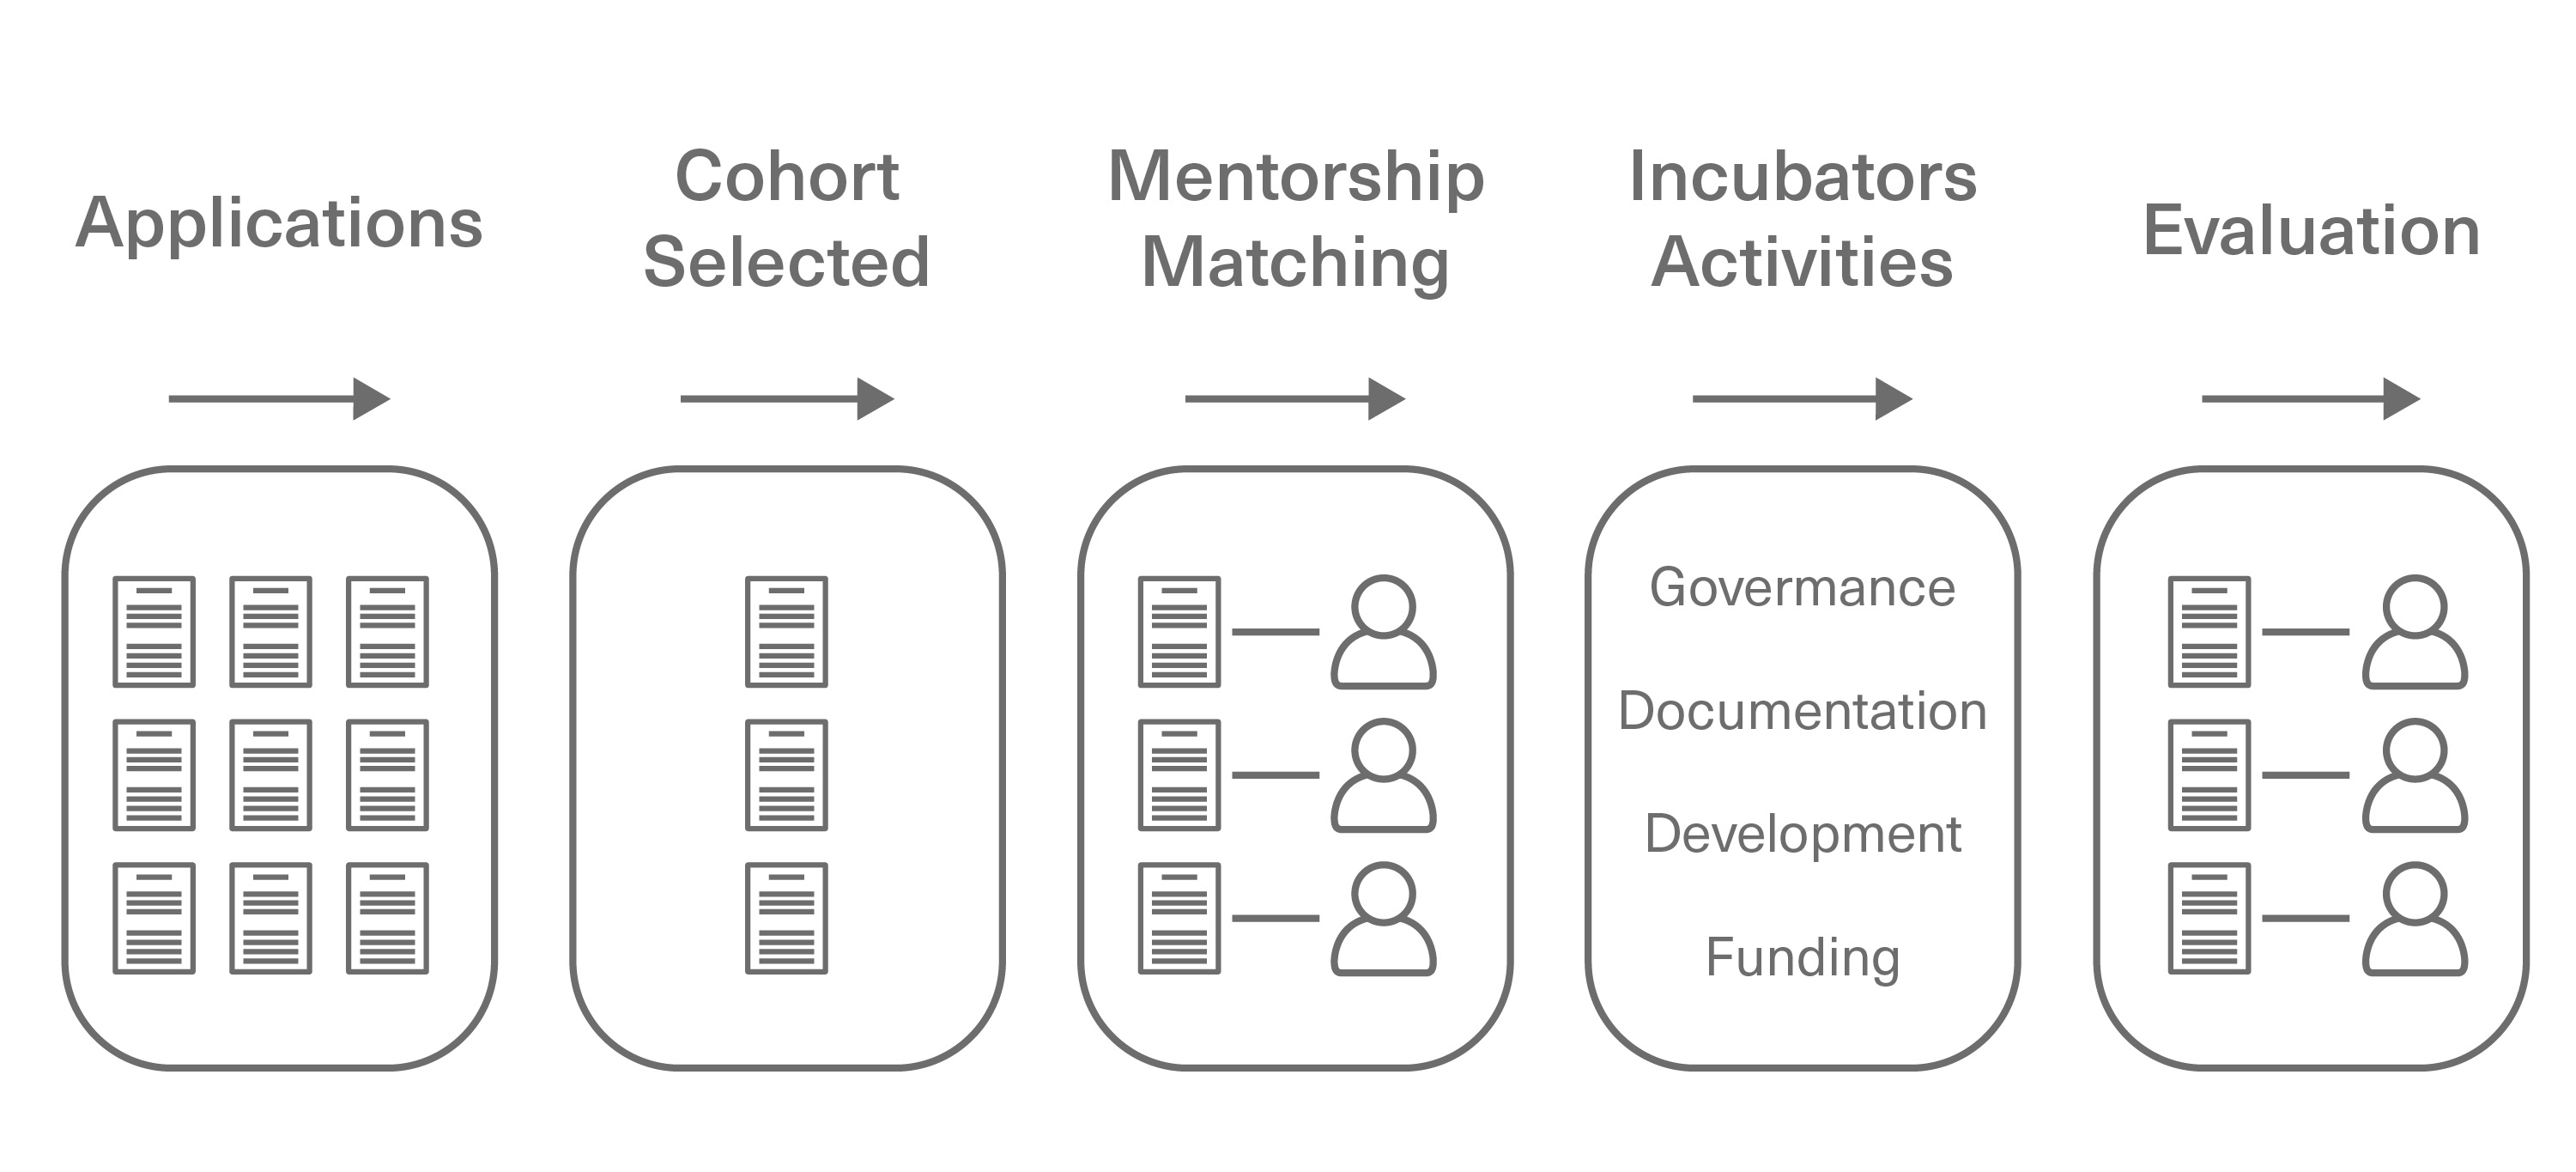
\includegraphics{images/URSSI-Incubator.jpg}
\caption{A general depiction of how the URSSI Incubator may be organized}
\end{figure}

\textbf{Project roles}\\
The project lead will, under the guidance of the mentor and program lead, establish a formal definition of roles that a project member is to play.
If a project already has a set of predefined roles then those roles will be reviewed for improvement, and formally documented.

\begin{itemize}
\tightlist
\item
  Roles will likely be similar across projects, but can and should leave some room for interpretation depending on the maturity of the project and the project's stated goals.
\item
  Formally defining roles within the project is meant to ensure transparency, encourage participation, and efficacy in onboarding new or explaining the expectations for contributing to a project. As an example, Node.JS defines \href{https://medium.com/the-node-js-collection/healthy-open-source-967fa8be7951}{three} roles for a project's governance:

  \begin{itemize}
  \tightlist
  \item
    A \emph{Contributor} is any individual creating or commenting on an issue or pull request
  \item
    A \emph{Committer} is a subset of contributors who have been given write access to the repository
  \item
    A \emph{TC (Technical Committee)} is a group of committers representing the required technical expertise to resolve rare disputes
  \end{itemize}
\end{itemize}

\textbf{Project governance}\\
In addition to defining roles, the project lead will, under the guidance of the mentor and Program Lead, establish a model of governing the project that is clear about expectations in how decisions are made, establishing a roadmap or release schedule, and adjudicating disputes that may arise.
(Note: URSSI does not have to develop this guidance from scratch, but can modify and adapt \href{https://opensource.guide/leadership-and-governance/}{existing guides} for research software.

In addition, a governance model should also include:

\begin{itemize}
\tightlist
\item
  Code of conduct - which can follow existing \href{https://opensource.guide/code-of-conduct/\%20as\%20a\%20guide}{best practice recommendations}
\item
  Process and expectation for citing software, acknowledging use, and authoring papers related to the project, including how credit should be given to different project contributors. (Jupyter has a very good \href{https://github.com/jupyter/governance/blob/master/papers.md}{model} for this governance documentation)
\end{itemize}

A key component of the governance model will be selecting a license which dictates the proper uses of the intellectual property of the project.

\textbf{Establishing best (or good enough) software engineering practices}\\
This components of the incubator will be provided by the URSSI Education \& Training area, and include, but not limited to activities such as:

\begin{itemize}
\tightlist
\item
  Version control management
\item
  Test coverage and code integration
\item
  Code reviews
\item
  Issue templates and tracking
\item
  Software design
\item
  Release management
\end{itemize}

\textbf{Documentation}\\
Incubator activities around creating or improving documentation related to a software project will include guidance for creating helpful ReadMe files (e.g.~WriteTheDocs' \href{https://www.writethedocs.org/videos/na/2016/write-the-readable-readme-daniel-beck/}{recommendations}) on readable readme documentation{]}, project descriptions, creating style guides for documentation, and review of documentation with a technical writer.

\textbf{Project funding \& financial planning}\\
The project team should develop a policy for accepting donations, managing funds, seeking grants, etc. After a project lead formalizes this policy, it should be added to the governance documentation.

\textbf{Project evaluation}\\
Projects would, under the guidance of the program lead and mentors, establish appropriate metrics to track (e.g.~following guidance from the open source handbook on \href{https://opensource.guide/metrics/}{metrics}).
Guidance on this work will be informed by the metrics work URSSI is engaged in through its Policy area.
These metrics could include a number of potential evaluations:

\begin{itemize}
\tightlist
\item
  Discovery - CodeMeta or appropriate metadata is created for the repository to be discovered and reused
\item
  Usage - formal citations, stars or forks on GitHub, etc.
\item
  Contribution / Maintenance
\item
  Retention of contributors or maintainers
\end{itemize}

\hypertarget{project-graduation-or-exit}{%
\subsection{Project graduation or exit}\label{project-graduation-or-exit}}

Upon completion of the activities described above, a project will go through an Exit Evaluation. This evaluation will include four components:

\begin{enumerate}
\def\labelenumi{\arabic{enumi}.}
\tightlist
\item
  The project will publish a software paper in JOSS or similar domain journal.
\item
  The project mentor will then provide structured feedback to the project lead, and allow the project lead to reply or address any concerns raised in the feedback
\item
  The Project Lead will provide a very short recorded presentation to review the progress made on goals stated in the project proposal, activities completed, and demonstrate working software products for evaluation.\\
\item
  The URSSI Incubator Selection Committee (described above in the Selection subsection) will convene annually to review each cohort's materials - including the JOSS publication, the mentor review, and the project lead's presentation. The committee will vote on whether or not the project should graduate from the Incubator.
\end{enumerate}

Graduation from the Incubator should send a positive signal about the sustainability of the project, but should not be a formal credentialing mechanism or certification of guaranteed sustainability.
Similar to other incubator programs (e.g.~YC, or Apache) graduation should be viewed as a significant achievement in itself.

\hypertarget{relationship-to-funding-and-external-awards}{%
\subsection{Relationship to funding and external awards}\label{relationship-to-funding-and-external-awards}}

An incubated project could have a relationship to external funding or funders in a variety of ways.
Most significantly, we view the incubator as a potential matchmaker between promising research software projects and potential funders.
Thus, funders will be invited and are an important participant in the Incubator showcase or graduate events.

Successfully graduating from the incubator program should act as an informal signal to funders that the project has the potential for further investment.
In this scenario, completing the URSSI Incubator would act as an informal quality check.
Funders would have greater assurance about the potential for a project to succeed, for funding new directions of the project, or potentially funding an institution or group around the project so as to better support sustainability.

\hypertarget{incubator-metricsmilestones}{%
\section{Incubator metrics/milestones}\label{incubator-metricsmilestones}}

For Incubated projects there will be two periods of evaluation.

Short-term evaluation (1-2 years):

\begin{itemize}
\tightlist
\item
  Increase in the number of mentions in research projects on GitHub, publications, and software dependencies compared to other research software of similar age.
\item
  Increase in the number of GitHub stars, forks, downloads (from package managers) relative to other projects of similar age that have not gone through the incubation process.
\item
  Improvement in codebase, documentation, governance, licensing, or strategic planning. This improvement can be defined with project mentors that set specific targets or goals for individual projects.
\end{itemize}

Long-term evaluation (3-5 years):

\begin{itemize}
\tightlist
\item
  Number of projects that attract follow-on funding
\item
  Persistence - This could be measured by the number of projects that continue to exist 5 years from incubator graduation, software that has regular contributions or updates to the repository, and active maintainers that have been identified as part of the project for different stages of development.\\
\item
  Attracted contributors - This could be measured over a portion of time that looks at commit history of different individuals contributing to a repository.
\item
  Returning Mentors - This could be measured by mentors who had graduated the incubator and return to provide guidance and help to new incubator projects.
\end{itemize}

For the Incubator program evaluation may include any of the following:

\begin{itemize}
\tightlist
\item
  In years 1-3 URSSI will select at least 15 projects (\textasciitilde{} 5 per year) for incubation. The program should be evaluated based on the success of projects' graduating from the Incubator, and whether or not those projects meet both short and long term milestones (as described above).\\
\item
  Funders participation (i.e., that the program attracts funded projects to enter and exit URSSI Incubator)
\end{itemize}

\textbf{Impacts:}

While in other chapters, we have mapped the activities from that chapter to the three portions of URSSI's intended impact,
here we treat the incubator as a single activity.
(A complete table of impacts from all URSSI activities can be found in \href{Ch-Metrics}{Chapter 10 (Metrics and Evaluation)}.)

\begin{table}

\caption{\label{tab:unnamed-chunk-3}Impact table}
\centering
\begin{tabular}[t]{lccc}
\toprule
Activity & Impact on Research Software & Impact on people and careers & Impact on research software ecosystem\\
\midrule
Incubator & X & X & \\
\bottomrule
\end{tabular}
\end{table}

\hypertarget{Ch-Policy}{%
\chapter{Policy}\label{Ch-Policy}}

The Policy area's intent is create an enabling environment to support the people who develop and maintain research software, and to
support research about research software, to ultimately increase the science \& research impact of
software.\\
\textbf{The Policy area's activities are divided into two parts, research and advocacy}. Research is the collecting
and analyzing of data, while advocacy is the dissemination of the research results in such a way that it
changes practices.
The Policy area focuses on understanding and then advocating for potential initiatives (actions, mandates, incentives, directives)
that decision makers can take, sometimes thought of as leverage points,
including strategies and decisions to invest. Policy happens at multiple levels, including national,
funding agency, institution, and research group.

The Changes that the Policy area seeks to make include:

\begin{enumerate}
\def\labelenumi{\arabic{enumi}.}
\item
  In funding agencies, direct funding of software maintenance and other software sustainability activities
  is a core part of the mission, e.g., at NSF, this includes all program officers across all directorates.
\item
  In universities and academic fields, positions for people developing and maintaining research software
  are available, recognized, and rewarded.
\item
  In publishing, support and recognition for software as a core part of scholarly research is the norm.
  (This includes the recognition that software is as valuable to the research community as the results themselves,
  that processes exist to evaluate software in papers, expectations for authorship for software developers are clear.)
\item
  In industry, sharing best practices, coordinating efforts, and contributing to open source software
  projects is the norm.
\item
  Open source software is recognized as a key element of open science and reproducibility.
\item
  Research software is built and maintained by a diverse and inclusive group.
\end{enumerate}

\hypertarget{policy-resources}{%
\section{Policy resources}\label{policy-resources}}

The policy area will require resources that include funding for people and for events and travel.

\hypertarget{people}{%
\subsection{People}\label{people}}

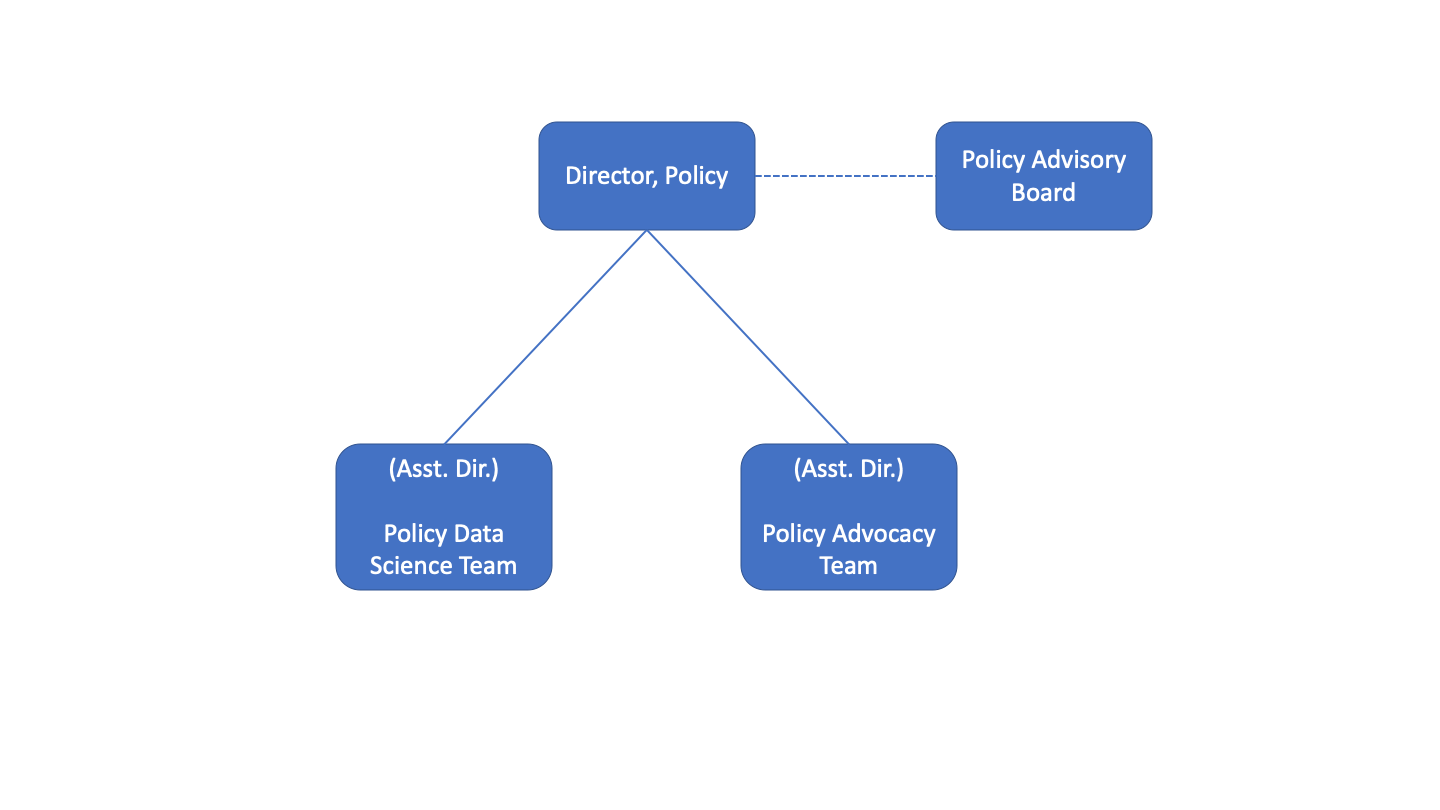
\includegraphics{images/policy_structure.png}

The policy area comprises:

\begin{itemize}
\item
  Director for Policy, an URSSI co-PI, leads the overall Policy area, working with the
  Policy Advisory Board and Policy staff to define and execute policy research and advocacy activities.
\item
  Policy Data Science Team: performs research such as finding, collecting, and analyzing data,
  aimed at informing policy, but not about policy
  itself. For example, with regard to software usage metrics, empirical studies would be most effective,
  but this team would not recommend policy language based on those studies.
  Includes a possible assistant director, funded staff, URSSI fellows, and community volunteers.
\item
  Policy Advocacy Team, focused on policy development (such as use cases and examples of practices
  that are effective for sustainability), which ultimately would be used for presenting actionable ways
  to support research software to institutions, possibly integrating and building upon the data science
  teams findings. This team focuses more on planning advocacy that in doing it,
  by understanding different stakeholders, and building a roadmap for how to effectively advocate
  (within universities, foundations, industry, national labs, etc.)
  Includes a possible assistant director, funded staff, URSSI fellows, and community volunteers.
\item
  Policy advisory board (appointed volunteers) who provide advice on potential policy area
  research questions and advocacy activities.
\end{itemize}

\textbf{Funding for personnel}:

\begin{itemize}
\tightlist
\item
  3 FTEs, divided across possibly part-time Assistant Directors for Policy Data Science and Policy Advocacy,
  the Policy Data Science Team (potentially a postdoc), and the Policy Advocacy Team.
  The Director for Policy might also act as one of the Assistant Directors, depending on that person's background.
\end{itemize}

Additional team members, not funded by the policy area:

\begin{itemize}
\tightlist
\item
  Director for Policy, an URSSI co-PI, funded by URSSI at top level
\item
  Policy Advisory Group (appointed volunteers)
\item
  URSSI fellows, working in Policy Data Science Team and Policy Advocacy Team

  \begin{itemize}
  \tightlist
  \item
    (Fellows program to be run by URSSI \protect\hyperlink{Ch-Comm}{Community} area; these policy fellows might
    be funded by policy area if needed)
  \end{itemize}
\item
  Other community volunteers, in Policy Data Science Team and Policy Advocacy Team
\end{itemize}

\hypertarget{additional-resources}{%
\subsection{Additional resources}\label{additional-resources}}

Additional resources may be needed by the research group for data collection, management, analysis, etc.,
and by the advocacy team for dissemination of materials and community organization and support.
Both teams may need additional resources for producing materials, including graphic design, copy editing, etc).
Amount are \textbf{TODO} TBD

\hypertarget{events-travel}{%
\subsection{Events \& travel}\label{events-travel}}

\textbf{Funding for workshops}: \textbf{TODO}: TBD

\begin{itemize}
\tightlist
\item
  Potentially including a policy conference / workshop(s) akin to Aspen Institute or CODATA - \$370k.
  This could also could be part of an annual URSSI event. Some events might also be low/no cost, held fully virtually.
\end{itemize}

\textbf{Funding for travel/speaking}: \textbf{TODO}: TBD

\begin{itemize}
\tightlist
\item
  As part of advocacy activities, URSSI personnel will discuss findings and recommendations.
\end{itemize}

\hypertarget{flexibility}{%
\subsection{Flexibility}\label{flexibility}}

If there is less budget available, we would cut back on workshop funding

If there is more budget available, we would:

\begin{itemize}
\item
  Expand policy program to have a summer program for undergraduate and graduate students focused
  on software / science policy (e.g., an \href{https://www.nsf.gov/crssprgm/reu/faculty.jsp}{NSF REU site} or something like a Google Summer of Code for policy / law students)
\item
  Hire communication staff to do outreach and engagement around policy topics (dedicated
  expertise in policy as opposed to general outreach)
\end{itemize}

\hypertarget{policy-methods}{%
\section{Policy methods}\label{policy-methods}}

Initial activities are planned around an initial set of aims articulated below, where additional
aims also will be suggested. The URSSI leadership group will regularly review suggestions
of new aims, and will determine a rough desired level of activity across the aims.

The policy team will then develop and scope activities to match these desired levels, with review
from the Policy Advisory Board, which will also be able to suggest adding or removing aims
back to the leadership group.

The policy team will also maintain this listing of active, planned, and potential activities and
its mapping to the aim. Activities will be split into those that, if successful, are likely
to lead to significant changes in 1-2 years, 3-5 years, and longer-term, with an initial goal of
applying 50\% of resources to the 1-2 year activities, 40\% to the 3-5 year activities, and 10\% to
the longer-term activities.

\hypertarget{aims}{%
\subsection{Aims}\label{aims}}

Initially, the policy area will work to address the following set of aims:

\begin{enumerate}
\def\labelenumi{\arabic{enumi}.}
\tightlist
\item
  Establish career paths (including titles and evaluation criteria for hiring and promotion).
\end{enumerate}

\begin{itemize}
\tightlist
\item
  addresses Changes 2, 5 (from list of changes at the start of this chapter)
\item
  aims primarily at the people and careers portion of URSSI's impact goal, and secondarily at the research software ecosystem portion
\end{itemize}

\begin{enumerate}
\def\labelenumi{\arabic{enumi}.}
\setcounter{enumi}{1}
\tightlist
\item
  Improve the measurement of impact of individuals, especially in activities that are inherently
  collaborative like software development.
\end{enumerate}

\begin{itemize}
\tightlist
\item
  addresses Changes 1, 2, 3
\item
  aims primarily at the people and careers portion of URSSI's impact goal, and secondarily at the research software ecosystem portion
\end{itemize}

\begin{enumerate}
\def\labelenumi{\arabic{enumi}.}
\setcounter{enumi}{2}
\tightlist
\item
  Incentivizes contributions to public goods / infrastructure within the academic credit model
\end{enumerate}

\begin{itemize}
\tightlist
\item
  addresses Changes 1, 3, 5
\item
  aims primarily at the research software sustainability portion of URSSI's impact goal, and secondarily at the people and careers and research software ecosystem portions
\end{itemize}

\begin{enumerate}
\def\labelenumi{\arabic{enumi}.}
\setcounter{enumi}{3}
\tightlist
\item
  Disentangle software quality and software impact.
\end{enumerate}

\begin{itemize}
\tightlist
\item
  addresses Changes 1, 4, 5
\item
  aims at the research software ecosystem portion of URSSI's impact goal
\end{itemize}

\begin{enumerate}
\def\labelenumi{\arabic{enumi}.}
\setcounter{enumi}{4}
\tightlist
\item
  Better recognize the value and importance of software.
\end{enumerate}

\begin{itemize}
\tightlist
\item
  addresses Changes 1, 2, 3, 5
\item
  aims at the research software ecosystem portion of URSSI's impact goal
\end{itemize}

\begin{enumerate}
\def\labelenumi{\arabic{enumi}.}
\setcounter{enumi}{5}
\tightlist
\item
  Improve/increase funding opportunities and stable funding for maintenance of software that
  is important but doesn't have a generic market and/or isn't considered novel in the eyes of the
  average funder/reviewer. Today ``lumpy'' project funding (projects that are
  competitively funded for fixed periods, often with gaps between funded project periods) means
  that maintenance/sustainability can't be reliably folded into project costs.
\end{enumerate}

\begin{itemize}
\tightlist
\item
  addresses Changes 1, 4, 5
\item
  aims primarily at the research software ecosystem portion of URSSI's impact goal, and secondarily at the research software sustainability portion
\end{itemize}

\begin{enumerate}
\def\labelenumi{\arabic{enumi}.}
\setcounter{enumi}{6}
\tightlist
\item
  Increase the diversity of the development and maintenance community to achieve the diversity of the overall US population.
\end{enumerate}

\begin{itemize}
\tightlist
\item
  addresses Change 6
\item
  aims primarily at the people and careers portion of URSSI's impact goal, and secondarily at the research software ecosystem portion
\end{itemize}

\hypertarget{partners-1}{%
\subsection{Partners}\label{partners-1}}

The Policy area will seek to work with partners listed in the ``Partners'' section of \protect\hyperlink{chapter3}{Chapter 3}, specifically including:

other NSF SI2/CSSI Institutes \& Centers of Excellence
(e.g.~\href{https://sciencegateways.org}{SGCI}, \href{https://molssi.org}{MolSSI}, \href{https://iris-hep.org}{IRIS-HEP}),
the \href{https://www.researchsoft.org}{Research Software Alliance},
the \href{https://software.ac.uk}{Software Sustainability Institute},
the \href{https://us-rse.org}{US-RSE Association},
the (UK) \href{https://society-rse.org}{RSE Society},
the \href{https://www.academicdatascience.org}{Academic Data Science Alliance},
the \href{https://www.rd-alliance.org}{Research Data Alliance},
the \href{https://www.aaas.org/programs/science-technology-policy-fellowships}{American Association for the Advancement of Science (AAAS) Science \& Technology Policy Fellows},
\href{https://carcc.org}{CaRCC},
\href{http://www.oecd.org}{OECD},
and any other projects and organizations that also seek to define and address overlapping aims.

The Policy area needs to build relationships with the following groups and organizations, and
to work closely with them, particularly in policy activities.

\begin{itemize}
\item
  Institutional and research leaders in the academic and national laboratory community, such as
  VCRs, CTOs/CIOs, who can help URSSI penetrate various institutions and disciplines
\item
  Representatives from professional academic associations
\item
  Representatives from industry (including those already invested and sold on OSS, as well as
  those skeptically interested)
\item
  Representatives from Open Source communities, particularly those that are already effective and working at scale
\item
  People working in science policy, such as in AAAS and the National Academies (in particular, AAAS policy fellows might be interested in helping on time-constrained activities that match the purpose and period of their fellowship)
\item
  Representatives from organizations and companies serving OSS and RSE communities
  (e.g.~\href{https://numfocus.org}{NumFOCUS}, \href{https://codeforscience.org}{Code for Science \& Society}, GitHub, Code Ocean)
\item
  Representatives from organizations that represent other research support roles
  (e.g., librarians, data stewards, RSEs), to work together to promote all such roles
\item
  Representatives from organizations that focus on diversity and inclusion in academia,
  to encourage them to include software-focused roles where possible
\item
  People from the European Commission regarding European Open Science Cloud (EOSC), etc.
\item
  Representatives from organizations like the Research Data Alliance and FORCE11
\end{itemize}

\hypertarget{planned-activity-pool}{%
\subsection{Planned Activity Pool}\label{planned-activity-pool}}

This is the initial list of activities that URSSI will maintain, and choose from. The specific
activities that will be chosen to start depend on the funding level for URSSI. Most activities
include an amount of effort (generally in person-months) that is needed to accomplish them.
Note that some activities (the items below) include
raising additional funds for those activities - that fund raising is part of the activity. Other
activities (in the ``Unplanned Activity Pool'' subsection) are tracked but are beyond the scope of URSSI, and are more
likely activities that others might perform, potentially in coordination with URSSI.

Activities are divided into two types:

\begin{enumerate}
\def\labelenumi{\arabic{enumi}.}
\item
  \textbf{Policy Research Activities}. These activities involve research, such as gathering and analyzing evidence and data.
\item
  \textbf{Policy Advocacy Activities}. These activities focus on advocacy. They generally depend on policy research or previously
  gathered evidence and data.
\end{enumerate}

High-level activities include:

\begin{itemize}
\item
  Maintaining the list of potential activities and prioritizing them, including getting inputs
  from the overall community. These inputs will be collected and recorded by all members of the
  project in their interactions with the community, as well as by community members, via tagged
  GitHub issues. Community members will be able to see this list and react with a +1 to issues
  they think are important, and URSSI will use these reactions as an element of prioritization. (ongoing)
\item
  Tracking completed activities and their consequences (ongoing)
\item
  Collecting examples of good and bad policy, structures, and interventions from industry and
  from other disciplines (potential fellow project)
\item
  Developing an advocacy roadmap for how to effectively advocate (to universities, foundations,
  industry, national labs) (policy person \& advisory committee, spread over 3 months)
\end{itemize}

Additionally, while this is a plan and not a proposal (it doesn't have a budget envelope it is working to fit in,
it is not responding to a specific solicitation, and the potential funder's goals are unclear) we have
considered priorities for these activities. Initial activities will mostly focus on research, as most advocacy
activities would follow and be based on the results and lessons of the research activities. In addition,
as mentioned above, final prioritization will also need inputs from the Policy Advisory Board and the URSSI
leadership team. Activities with a preceding ``(+)'' are considered higher priority than other activities.

\hypertarget{career-path-activities-aim-1}{%
\subsubsection{Career Path Activities (Aim 1)}\label{career-path-activities-aim-1}}

\textbf{Faculty career path policy research activities}:

\begin{itemize}
\tightlist
\item
  Study tenure guidance and policies, and find/document ways that software work is measured
  and recognized. Publish examples of successes.
  (ADSA is interested in partnering on this; the ADSA Career Development Network is mostly faculty facing exactly these challenges.
  Additionally, RDA is in the processing of developing an \href{www.openscienceregistry.org}{Open Science Registry}\footnote{This link may not yet work.}
  as a collaborative platform to share both the intention and outcomes of pilots
  and other initiatives that specifically address the academic reward system, as an outcome of the
  European Union Open Source Policy Platform (OSPP) final report \citep{OSPP_report}.) (2 months)
\end{itemize}

\textbf{Faculty career path policy advocacy activities}:

\begin{itemize}
\item
  Promote best practices in recognizing and measuring software work in hiring practices and
  tenure letters via sample guidance documents for committees, for faculty, and for
  letter-of-reference authors. (needs focused workshop and follow-through, \textasciitilde3 months over a year)
\item
  Commission a NAS report (similar to the one on \href{https://www.nap.edu/read/25217/chapter/1}{Open Source Software Policy Options for NASA
  Earth and Space Sciences}) on career pathways/progression
  in academia. Would need to define, then raise funds from
  outside URSSI (\textasciitilde\$1m), then work with NAS to define a charge and to contract for the study.
  (4 months over 2.5 years, overlapping with related item in staff career path policy advocacy activities)
\end{itemize}

\textbf{Staff career path policy research activities}:

(All the activities below will be coordinated with US-RSE and other national RSE organizations. Additionally, some information already exists that can be mined, such as international and national RSE surveys \citep{rse-survey}, \ldots)

\begin{itemize}
\item
  (+) Document existing (known successful/viable, known failures) career paths for individuals
  creating research software (2 months)
\item
  (+) Examine and document industry career paths vs.~national laboratory career paths vs.~academic career paths (1 month)
\item
  (+) Create and maintain a mailing list for those interested in career paths (mailing list to be
  supported by Community area) (ongoing, low level of effort)
\item
  Create a clearinghouse of job descriptions with criteria for performance assessment; distill
  out design patterns or different categories for different roles. This could also include documenting
  salary levels for different job descriptions, and connecting the job descriptions with then learning
  modules necessary for these jobs (3-4 months, plus ongoing maintenance)
\item
  Examine how salaries for RSEs compare with those of other researchers? (needs to follow clearinghouse, 1 month)
\end{itemize}

\textbf{Staff career path policy advocacy activities}:

\begin{itemize}
\item
  (+) Help start organizational ``chapters'' of research software developers (perhaps called URSSI chapters?) at existing
  universities / societies / organizations; create handbook, tools, best practices to support
  local organizers; assign an URSSI ``coordinator'' / community manager. These chapters could:
  talk about training, do consulting for problems, host hacky hours, study groups, software days,
  and come together in a larger event, perhaps a regional workshop or an URSSI-wide conference. Overall, this
  helps / grows / establishes the community (and make connections that could help chapter members
  meet the right person for their next career moves).

  \begin{itemize}
  \item
    Done with URSSI \protect\hyperlink{Ch-Comm}{Community} area; Policy part (1 month) is creating some materials,
    e.g., guidance on how to set up a chapter, how to align it to local activities, and how to run it.
  \item
    Also to be coordinated with US-RSE, as regional US-RSE groups might overlap regional URSSI chapters.
  \end{itemize}
\item
  Work to promote and support the establishment of RSE capabilities at universities around the US.
  Provide advice on how to talk to university administrators (and which ones) about this, etc. (1 month,
  jointly with US-RSE)
\item
  Provide examples of language to universities they can use in HR/job ads for RSE positions
  (1 month, jointly with US-RSE)
\item
  Commission a NAS report (similar to the one on \href{https://www.nap.edu/read/25217/chapter/1}{Open Source Software Policy Options for NASA
  Earth and Space Sciences}) on
  \{career pathways/progression in academia, recognition of software, evaluation of software developers,
  inclusion of software in hiring and promotion\} Would need to define, then raise funds from
  outside URSSI (\textasciitilde\$1m), then work with NAS to define a charge and to contract for the study.
  (4 months over 2.5 years, overlapping with related item in faculty career path policy advocacy activities)
\end{itemize}

\hypertarget{the-impact-of-individuals-aim-2}{%
\subsubsection{The impact of individuals (Aim 2)}\label{the-impact-of-individuals-aim-2}}

\textbf{The impact of individuals policy research activities}:

\begin{itemize}
\tightlist
\item
  Identify factors (manual, such as evaluations, and automated, such as crawling repos) that are
  part of impact and publicize them. Some known factors to investigate include quantifying code
  contributions, code review, mentoring. Determine good practices (for formatting or housing the
  information on these factors) so those factors are discoverable and/or queryable.
  (An initial effort of 6 months will make progress and better scope additional work that could be performed.)
\end{itemize}

\textbf{Measuring the impact of individuals policy advocacy activities}:

\begin{itemize}
\item
  Create champions (e.g.~librarians) to promote and educate individuals and projects of these
  good practices, working with the best practices activity in \protect\hyperlink{Ch-Comm}{Community area}.
\item
  Help individuals understand how they can best promote themselves (e.g., claim software works on
  ORCID), working with the best practices activity in \protect\hyperlink{Ch-Comm}{Community area}.
\end{itemize}

\hypertarget{incentivize-contributions-to-public-software-aim-3}{%
\subsubsection{Incentivize contributions to public software (Aim 3)}\label{incentivize-contributions-to-public-software-aim-3}}

\textbf{Incentivize contributions to public software policy research activities}:

\begin{itemize}
\item
  Gather data/examples that show when contributions to public projects increase your citation
  count or regular metrics (1 month)
\item
  (+) Gather examples of successful use of individual contributions to public goods/infrastructure
  to gain academic promotion (1 month over 3-6 months)
\item
  (+) Use regular surveys to better understand why people do and don't contribute; get data to
  understand the value of public goods to community (1 month over 3-6 months each year)
\item
  Determine a way to make it easy for scientific communities to peer-review public-good software
  (or contributions to such software), with the idea that peer-review is considered a mark of
  quality. This could be done by starting a new journal or working with existing journals or conferences,
  or via existing community organizations or software-focused organizations (ongoing, not well-scoped)
\item
  Research to counter the idea that publishing in the small set of ``highest impact'' journals is
  key, and expose actual impact of work instead (work with scholcom community, use what they have
  done, maybe adapt their work for software - maybe 2 months to start)
\end{itemize}

\textbf{Incentivize contributions to public software policy advocacy activities}:

\begin{itemize}
\item
  Work to persuade high-profile individuals to make public contributions to public projects
\item
  (+) Share examples of successful use of individual contributions to public goods/infrastructure
  to gain academic promotion, produce templates, advocacy toolkits and examples to help others
  to make their case. Similarly, work to persuade people that contributing to projects will
  increase their products within their normally accepted reward system (e.g., get more collaborators
  and papers; increase opportunities to meet/work with new/old collaborators; will build social
  connections/network) (ongoing, not well-scoped)
\item
  (+) Show how you can participate in public goods / infrastructure projects (e.g., how to
  structure an issue, how to write your first PR), collaboratively with best practices activity in
  URSSI \protect\hyperlink{Ch-Comm}{Community} area (low initial effort, low ongoing effort to maintain)
\item
  Produce templates based on successful use of individual contributions to public
  goods/infrastructure to gain academic promotion, advocacy toolkits, and examples to help
  others to make their case (1 month)
\item
  Reframe contributions as first class research products / objects (i.e., explain how building
  the best software is itself science, as it's both discovery and creation). In order to do this,
  amplify existing efforts to build a taxonomy of such contributions to make it clear what those
  contributions are, and encourage people to claim/talk about/take pride in these contributions;
  work with publishers to highlight these contributions and the people who make them. Also advocate
  (materials, webinars, ambassadors, etc.) within academic communities (deans, faculty, science
  societies, review panels, funders) that public software contributions are research (also could
  be done by cross-disciplinary respected groups, such as the national academies)
\item
  (+) Work to revise funder policies to ensure reviewers prioritize grant proposals that reuse,
  build-upon and contribute back to maintenance of public infrastructure
\item
  Create high-profile equivalent of ``highest impact'' journal for software and data work - where publication
  is seen as an accomplishment indicating the significance of the software
\end{itemize}

\hypertarget{disentangle-software-quality-and-software-impact-aim-4}{%
\subsubsection{Disentangle software quality and software impact (Aim 4)}\label{disentangle-software-quality-and-software-impact-aim-4}}

\textbf{Disentangle software quality and software impact policy research activities}:

\begin{itemize}
\tightlist
\item
  Create checklists/review guidelines for different levels of peer-review for software; can be
  tiered, could issue stars or use another rating system; leverage information already available
  from journals and other resources. (1 week)
\end{itemize}

\textbf{Disentangle software quality and software impact policy advocacy activities}:

\begin{itemize}
\tightlist
\item
  Disseminate peer-review for software checklists/review guidelines to publishers and other organizations
  that review software, via a working group. (2 months over 2 years)
\end{itemize}

\hypertarget{better-recognize-the-value-and-importance-of-software-aim-5}{%
\subsubsection{Better recognize the value and importance of software (Aim 5)}\label{better-recognize-the-value-and-importance-of-software-aim-5}}

\textbf{Recognize the value and importance of software policy research activities}:

\begin{itemize}
\item
  (+) Find science/discovery cases where software was particularly fundamental, particularly digging
  into software that is not so generally well-known (2 months over 6 months)
\item
  (+) Research and deliver case studies in sustainable software value, e.g., NetCDF, HDF5, DS9 image viewer,
  GCM model(s). How much money was invested in these projects and how did these projects return value to
  the community? Examples of value could include: number of research projects taking advantage of these
  solutions, amount saved by not having to reinvent these technologies. (6-to-12-month fellow project)
\item
  Quantify the money that has implicitly funded maintenance and sustainability, and has been saved
  or lost in the shift to open source (e.g., where have funds been spent on one-off software rather
  than maintaining existing open source software, and where has an investment in software maintenance
  saved funds from being spent on one-off software) (6-month fellow project)
\item
  Calculate bus factor for a bunch of key software in disciplines (partner with CHAOSS, or perhaps
  6-month fellow project)
\item
  Document maintenance and funding for critical packages for several disciplines, e.g.~IRAF in astronomy
  (6-month fellow project)
\end{itemize}

\textbf{Recognize the value and importance of software policy advocacy activities}:

\begin{itemize}
\item
  (+) Publicize science/discovery cases where software was particularly fundamental, focusing on
  demonstrating impact of software (1 week/year, ongoing)
\item
  (+) Raise awareness that software needs to be maintained (low level, ongoing)
\end{itemize}

\hypertarget{funding-opportunities-for-software-maintenance-aim-6}{%
\subsubsection{Funding opportunities for software maintenance (Aim 6)}\label{funding-opportunities-for-software-maintenance-aim-6}}

\textbf{Funding opportunities for software maintenance policy research activities}:

\begin{itemize}
\item
  (+) Review the landscape of funding opportunities for software maintenance (and gather data about them)
  and provide a public summary, then keep the summary up-to-date. (jointly done with ReSA? Or CZI EOSS?)
  (1 month and some ongoing work)
\item
  Gather case studies of successful commercialization of open source projects and encourage the
  research community to understand and make use of them (2 months)
\item
  Review the scope of maintenance needs by various research disciplines. Determine the order of
  magnitude of the maintenance backlog for research software (with CHAOSS and others, unscoped)
\end{itemize}

\textbf{Funding opportunities for software maintenance policy advocacy activities}:

\begin{itemize}
\item
  Encourage funding agencies to require software management/maintenance plans (SMPs).
  Use them to couple the idea of maintenance to the idea of development, to make it clear
  that just doing development without maintenance doesn't work. Note that this leads to
  questions about when maintenance should be stopped, and it's also unclear how long-term
  maintenance would be supported (since grants are by definition time-limited).
  (1-2 months/year ongoing, work with ReSA)
\item
  Advocate for funding agencies to provide a funding pool for short-term maintenance grants
  for existing projects (e.g.~CZI's EOSS program). (1-2 months/year)
\item
  (+) Advocate for universities to support maintenance of software developed by their university
  as part of research impact (or possibly technology transfer), in part by including how software
  we highlight in the success stories campaign was paid for, including university and RSE contributions,
  then using this collectively to demonstrate the impact of specific university-funded activities,
  to encourage other universities to step up. (2 months/year over multiple years)
\item
  Encourage companies to provide funds and channel these funds into maintaining research
  software projects, perhaps via a review process with reviewers from both academic software
  projects and the companies. This could be done jointly with NumFOCUS or a similar organization,
  similar to Tidelift (1-2 months/year)
\end{itemize}

\hypertarget{increase-diversity-of-software-community-aim-7}{%
\subsubsection{Increase diversity of software community (Aim 7)}\label{increase-diversity-of-software-community-aim-7}}

\textbf{Diversity and inclusion policy research activities}:

\begin{itemize}
\item
  (+) Survey US research software projects to examine diversity of leadership and contributors (3 months)
\item
  Study/survey contributors who make a single contribution and those who make ongoing contributions
  vs membership in underrepresented groups (3 months)
\item
  (+) Contribute to \href{https://discover-cookbook.numfocus.org}{DISCOVER event cookbook}, working with
  NumFOCUS's \href{https://numfocus.org/programs/diversity-inclusion}{DISC}
\item
  Other items with CS\&S and NumFOCUS's \href{https://numfocus.org/programs/diversity-inclusion}{DISC},
  for example, creating a cookbook aimed at projects
\end{itemize}

\textbf{Diversity and inclusion advocacy activities}:

\begin{itemize}
\item
  (+) Advertise \href{https://discover-cookbook.numfocus.org}{DISCOVER event cookbook}, working with
  NumFOCUS's \href{https://numfocus.org/programs/diversity-inclusion}{DISC}
\item
  (+) Other items with CS\&S and NumFOCUS's \href{https://numfocus.org/programs/diversity-inclusion}{DISC},
  such as advertising the cookbook aimed at projects
\item
  Reach out to projects to encourage them to mentor \href{https://www.outreachy.org}{Outreachy} interns
  and those from other programs (e.g.,
  \href{https://www.linuxfoundation.org/about/diversity-inclusiveness/programs/}{Linux Foundation diversity programs},
  \url{https://opensourcediversity.org/\#programs}), and to work with Google Summer of Code, maybe
  include some matchmaking. Consider URSSI as an organization that applies to a set of these
  programs on behalf of a set of software projects.
\item
  Build community mentoring program focused on diversity
\item
  Work with RLadies, Women in Data Science, etc.
\end{itemize}

\hypertarget{general-advocacy-activities-not-mapped-to-specific-aims}{%
\subsubsection{General advocacy activities (not mapped to specific Aims)}\label{general-advocacy-activities-not-mapped-to-specific-aims}}

\begin{itemize}
\item
  Work with REU\footnote{REU is refers to both \href{https://www.nsf.gov/crssprgm/reu/}{NSF's Research Experience for Undergradautes}
    program, as well as being a generic term for summer and other programs that provide undergraduates with research experience.}
  programs? -- set up a network of software-focused REUs? Or focus on software
  aspects of more REUs? (provide training, guidance, language for proposals, \ldots)
  (2 month to start + ongoing)
\item
  Foster competition between universities (and their administrations), as has been done by
  the SSI in the UK to create RSE groups, by:

  \begin{itemize}
  \item
    Highlighting software work (including internal investments to sustain projects that the
    university sees as important and prestigious) and successes (including funded projects that
    focus on software) in some universities.
  \item
    Ranking the contributions of universities to software or their structure for software developers,
    and publicizing the ranking (maybe with US-RSE) -- via newsletter, blogs, press releases
    (pontentally run by or at least coordinated with the URSSI community area). This could be based in
    part on information submitted by the software community, e.g.~Laura Noren's and Brad Stenger's Data
    Science Community Newsletter. These rankings and information would also be bi-directionally shared
    with ReSA.
  \end{itemize}
\item
  Work in citation and credit (get publishers to recognize and highlight software in
  research) (with FORCE11 and others) (minor support of other activities)
\item
  Promote software management plans and software sustainability plans as part of proposals
  (3 months over a year, bringing together community and volunteers, work with ReSA and RDA)
\item
  (+) Develop a set of options for how institutions can support research software (e.g., RSE groups,
  RSE careers, tenure and promotion guidelines) and disseminate it (with US-RSE, starting after year 1)
\item
  (+) Create and operate a professional award program (working with other established organizations)
  e.g., ESA URSSI software award. The URSSI software contribution to research awards: URSSI/ESA
  (e.g.~John Chambers software award from stats association). \$10k funding available from URSSI
  (eventually domain societies would be asked to partially fund the awards). URSSI would need to
  define the categories, criteria/heuristics, etc. for awards beforehand. And find people
  (either staff or community volunteers) to run awards processes (accept nominations, make decisions)
  (2 weeks/year starting in year 2)
\item
  (+) Work with NumFOCUS to provide guidance to projects on how to work with (including obtaining
  funding from) industry (sharing material with incubator area)
\item
  (+) Offer training for software development proposals (or point to others who do)

  \begin{itemize}
  \item
    Develop and disseminate best practices for software development proposals (with NumFOCUS or
    the Capentries)
  \item
    Training/materials could be asynchronous, or in-person with NSF program officers as well, if
    they were willing to do so
  \end{itemize}
\item
  Licensing (in partnership with OSI, Creative Commons, others)

  \begin{itemize}
  \tightlist
  \item
    Provide (pointers to) guidance on licenses and copyright for research software (little work,
    partner with OSI and point to existing best practices)
  \end{itemize}
\end{itemize}

\hypertarget{unplanned-activity-pool}{%
\subsubsection{Unplanned Activity Pool}\label{unplanned-activity-pool}}

The activities listed here are those that would support URSSI but are beyond the scope of URSSI.
They are listed here to provide ideas to others, and URSSI would potentially be willing to encourage
and support them, but likely without resources.

\hypertarget{staff-career-path-policy-research-activities-aim-1}{%
\paragraph{Staff career path policy research activities (Aim 1)}\label{staff-career-path-policy-research-activities-aim-1}}

\begin{itemize}
\tightlist
\item
  Comparative study of research success at universities with core RSE groups vs those without.
  (potential research topic, not to be started by URSSI)
\end{itemize}

\hypertarget{incentivize-contributions-to-public-software-policy-advocacy-activities-aim-3}{%
\paragraph{Incentivize contributions to public software policy advocacy activities (Aim 3)}\label{incentivize-contributions-to-public-software-policy-advocacy-activities-aim-3}}

\begin{itemize}
\tightlist
\item
  Run a help desk once a week on-line for people who are running into difficulties in making contributions and need help
\end{itemize}

\hypertarget{disentangle-software-quality-and-software-impact-policy-research-activities-aim-4}{%
\paragraph{Disentangle software quality and software impact policy research activities (Aim 4)}\label{disentangle-software-quality-and-software-impact-policy-research-activities-aim-4}}

\begin{itemize}
\item
  Define what software quality means.
\item
  Define what software impact means and how to measure it. Impact can be looked at in many
  ways: scientific, economic, societal, etc.
\item
  Define how you know what software will be impactful (signals of high impact)
\item
  Capture the difference between software quality and software impact in written resources (blog post, paper, etc.)
\item
  Conduct a Delphi study or multiple Delphi studies across or between disciplines to determine
  a consensus on key indicators of software impact and related questions, such as: Does improving
  the quality of software improve its impact?
\item
  Perform randomized experiments of software impact where the treatment is improved software practices
\item
  Perform a retrospective study of software quality as related to ``impact'' of that software.
\end{itemize}

\hypertarget{recognize-the-value-and-importance-of-software-policy-research-activities-aim-5}{%
\paragraph{Recognize the value and importance of software policy research activities (Aim 5)}\label{recognize-the-value-and-importance-of-software-policy-research-activities-aim-5}}

\begin{itemize}
\tightlist
\item
  Study whether higher-quality software produces higher-impact science or more reliable science results
\end{itemize}

\hypertarget{funding-opportunities-for-software-maintenance-policy-advocacy-activities-aim-6}{%
\paragraph{Funding opportunities for software maintenance policy advocacy activities (Aim 6)}\label{funding-opportunities-for-software-maintenance-policy-advocacy-activities-aim-6}}

\begin{itemize}
\item
  Provide a system to match open source maintenance needs and open source programmers
  (e.g., classified ads), to be funded by URSSI, or URSSI could support proposals for such
  maintenance work (both morally and by providing guidance to the proposer)
\item
  Provide fellowships for programmers to ``do good stuff'' related to maintenance
\item
  Attach money for maintenance to some of the to-be-created awards for good software
  development, jointly named and funded with other communities
\end{itemize}

\hypertarget{general-advocacy-activities-not-mapped-to-specific-aims-1}{%
\paragraph{General advocacy activities (not mapped to specific Aims)}\label{general-advocacy-activities-not-mapped-to-specific-aims-1}}

\begin{itemize}
\item
  Talk about problems with current software licenses/models and suggest alternatives
\item
  Create peer-review and publishing systems that are software appropriate, and not just a version of
  article appropriate system. For instance, find a software ecosystem-native way to peer-review software
  inside a code management system, or ``publish'' software by giving a specific version of code a DOI
\end{itemize}

\hypertarget{work-between-policy-and-other-urssi-areas}{%
\section{Work between Policy and other URSSI Areas}\label{work-between-policy-and-other-urssi-areas}}

\begin{itemize}
\item
  \protect\hyperlink{Ch-Edu}{Education \& Training} -- use to learn about problems, use training events to disseminate products and advocacy
\item
  \protect\hyperlink{Ch-Comm}{Community} -- provide topics for fellows, work with on newsletter and dissemination, host champions,
  contribute to and disseminate best practices
\item
  \protect\hyperlink{Ch-Incubator}{Incubator} -- develop both general and specific guidance for projects
\end{itemize}

\hypertarget{policy-metricsmilestones}{%
\section{Policy metrics/milestones}\label{policy-metricsmilestones}}

\begin{itemize}
\item
  Amount of funding provided by US public and private funding agencies for research software
  development and maintenance
\item
  Number and fraction of US universities with RSE-like positions, and number of such positions at each university
\item
  Number and fraction of US university faculty who successfully use software work as an important part of
  their tenure packages
\item
  Number of participants in policy events, and their satisfaction based on exit surveys
\item
  Collect ``thank yous'' and anecdotes where URSSI is recognized for helping do something
\item
  Number of requests from universities for talks from URSSI staff
\item
  Number of talks by others where URSSI is discussed
\item
  Number of views and citations of URSSI policy documents and web sites
\item
  \textbf{TODO}: more needed
\end{itemize}

\textbf{Impacts:}

This table maps URSSI activities from this chapter to the three portions of URSSI's intended impact.
(A complete table of impacts from all URSSI activities can be found in \href{Ch-Metrics}{Chapter 10 (Metrics and Evaluation)}.)
In the impact cells, X indicates a designed primary impact on an activity, and y indicates
a designed secondary impact.

\begin{table}

\caption{\label{tab:unnamed-chunk-4}Impact table}
\centering
\begin{tabular}[t]{lccc}
\toprule
Activity & Impact on Research Software & Impact on people and careers & Impact on research software ecosystem\\
\midrule
Career path &  & X & y\\
Impact of individuals &  & X & y\\
Incentivize contributions to public software & y & y & X\\
Disentangle software quality and software impact &  &  & X\\
Better recognize the value and importance of software &  &  & X\\
\addlinespace
Funding opportunities for software maintenance & y &  & X\\
Increase diversity of software community &  & X & y\\
Award program &  & y & X\\
\bottomrule
\end{tabular}
\end{table}

\hypertarget{Ch-Org}{%
\chapter{Management \& Coordination Area}\label{Ch-Org}}

The Management \& Coordination Area of URSSI is designed to manage the project (assign and monitor work,
usually in work packages; monitor, mitigate, and respond to risks; provide reports; adapt work to
community feedback; and ensure project sustainability) and foster collaboration between the four
other areas of URSSI: Policy, Education \& Training, Incubator, and Outreach \& Community.

\hypertarget{management-resources}{%
\section{Management resources}\label{management-resources}}

The PI and Co-PIs are funded at 0.25 FTE and are supported by staff at their home institutions for
writing reports and budgeting, etc. The Work Package Leader roles are filled by PIs and/or senior
personnel and are funded at around 0.1 FTE for leading a work package. The Sustainability Officer,
Diversity Officer and Evaluator are each planned at 0.1 - 0.25 FTE depending on the phase of the
institute. The initial phases of ramping up the institute, defining work packages (see definition below)
and services, as well as detailed project plans with 1-year to 5-year goals will require more effort
at the beginning, and we will revisit the level of effort after about 18 months and 48 months.
In addition to continuous monitoring of progress and risks and potential refactoring of work and
addressing risks, work on sustainability, evaluation and diversity, will be major topics.

\hypertarget{work-packages}{%
\section{Work packages}\label{work-packages}}

All work to be done in URSSI (including management and coordination) is structured into
work packages (WPs), which are organized around the project's goals and areas, with an additional
WP that is concerned with quality and risk management, project coordination, sustainability, and
reporting activities. A WP defines a discrete unit of work over some period, and can be part of
one or more areas. The duration of a WP can be a fixed period (e.g., six months to organize and
run a single training event) or can span the full lifetime of the project, such would be the case
for the maintenance of the website or regular distribution of newsletters. For example, a WP to
support a new open-source project might last a year and span three areas: education \& training,
incubator, and outreach \& community.

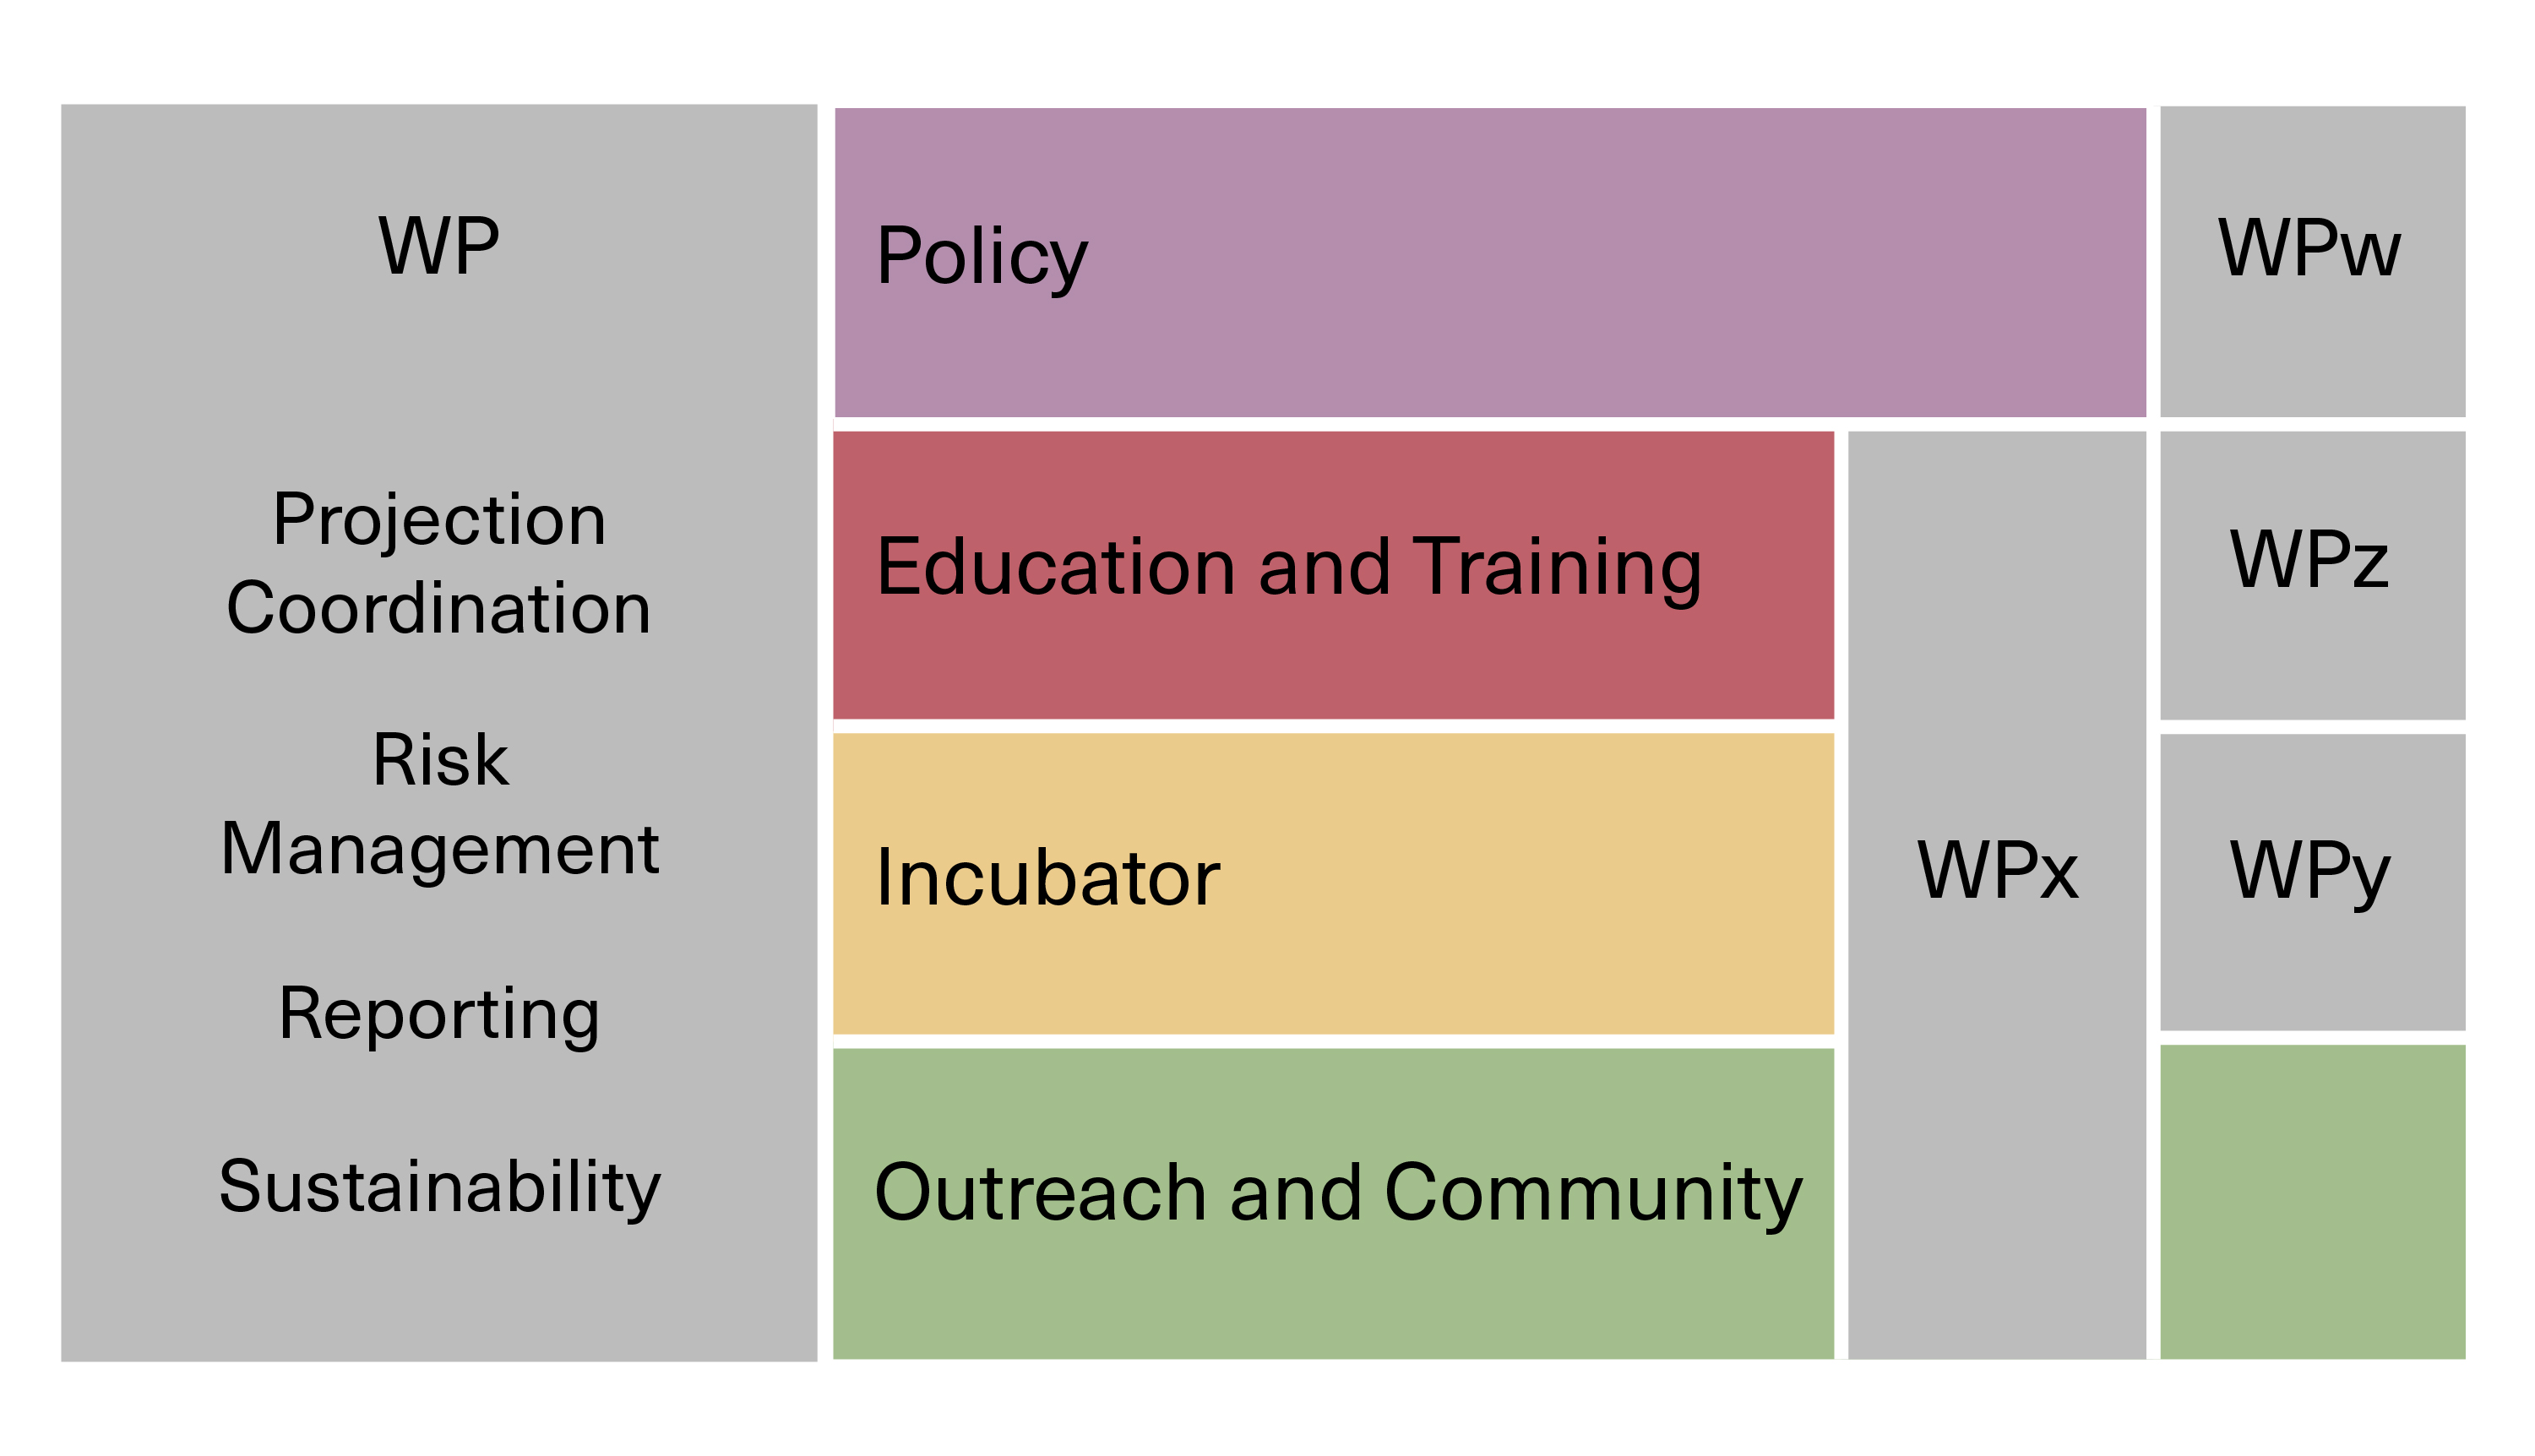
\includegraphics{images/WPs-v3.jpg}

Fig. Areas and WPs: A WP can exist in one or more areas. The WP ``Project coordination, risk management
and reporting'' spans all four areas and lasts for the duration of the project. WPx, for example, is
part of Education \& Training, Incubator, and Outreach \& Community. WPy, WPz, and WPw each exist in
a single area.

\hypertarget{management-structure-and-procedures}{%
\section{Management structure and procedures}\label{management-structure-and-procedures}}

Management of URSSI includes activities that occur at different levels, appropriate to the size and
structure of the institute. This section presents the project's organizational and decision-making
mechanisms, as well as its process for ensuring effective information interchange between the
individual work packages. Central to the project's management is a key set of roles and committees,
which are described in detail below: the PI, the Co-PIs, the Work Package Leaders, a sustainability
officer, an evaluator, and the Steering Committee. Work Package leaders may be Co-PIs or other URSSI staff.

The \textbf{PI and Co-PIs} have overall responsibility for project activities and will work with the
evaluator to make periodic revisions to ensure the project's continuing success.The PI will manage
the administrative and financial aspects of the project, with the assistance of one or two staff
members. The PI will also oversee the day-to-day management of the project, with the support of the
Co-PIs. The PI and Co-PIs are responsible for reviewing the overall progress of the project. They will
work closely with the Work Package Leaders to manage the technical work of the project.
\textbf{Work Package Leaders} will be responsible for the progress of their individual work packages, the
timely production and quality of deliverables, and the achievement of milestones.
The \textbf{Sustainability Officer} will work towards ensuring the sustainability of the overall institute.
The \textbf{Diversity Officer} will ensure that URSSI meets its internal and external diversity goals, and will
suggest additional activities as needed.
The \textbf{Evaluator} will ensure that URSSI activities progress towards the overall goals of URSSI are measured and,
and will suggest corrective actions when needed.
The \textbf{Steering Committee} will advise and support the PI and Co-PIs. \textbf{Senior Personnel} are
responsible for tasks assigned to them by Work Package leaders. Tasks include administrative tasks for the project.

This structure has been developed to:

\begin{itemize}
\tightlist
\item
  Ensure effective management of the project;
\item
  Ensure clearly defined communication channels both internal and external to the project;
\item
  Establish clear procedures for making decisions and resolving conflicts;
\item
  Ensure the project proceeds within the framework of the budget, including efficient reallocation of budget if necessary and according to administrative, financial, and legal principles defined by NSF; and
\item
  Ensure that the participants meet their obligations in the project.
\end{itemize}

\hypertarget{project-management-team}{%
\section{Project Management Team}\label{project-management-team}}

The project management team comprises

\begin{itemize}
\tightlist
\item
  Leadership Team (the PI and Co-PIs)
\item
  Work Package Leaders
\item
  Sustainability Officer
\item
  Diversity Officer
\item
  Evaluator
\item
  Senior Personnel
\end{itemize}

In addition to this team, the project will rely on a Steering Committee.

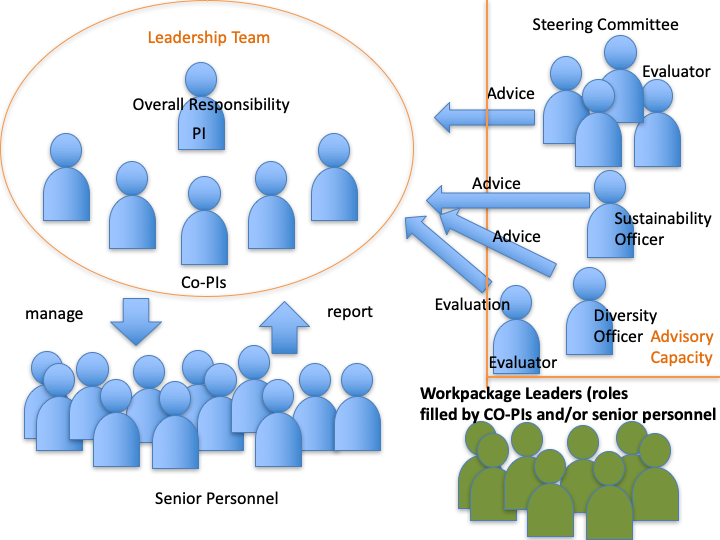
\includegraphics{images/managementStructure.png}

The Project Management Team will meet on an annual basis, starting with an initial meeting in the
first month of the project to promote effective and efficient work among all participants. This
meeting will include the whole project management team along with invited experts. The PI can call
additional meetings at any time. The annual meetings will be face-to-face when possible. Additional
meetings may be via telephone conference, video conference, or both. In addition to the core project
team, the PI can invite any person knowledgeable about an area of concern within the URSSI scope to
attend Project Management Team meetings in an advisory capacity.

The Project Management Team will contribute to the strategic orientation of the project and represents
the interests of all participants. Its main tasks are to:

\begin{itemize}
\tightlist
\item
  Collect feedback from potential user researcher communities and developer communities;
\item
  Disseminate the project's latest results via publications and presentations at conferences and workshops; and
\item
  Accomplish the work packages.
\end{itemize}

\hypertarget{steering-committee}{%
\subsection{Steering Committee}\label{steering-committee}}

The Steering Committee will be formed at the start of the project. It will consist of 6-8 experts invited
by the Leadership Team, drawn from diverse areas including sustainability, software engineering, and
domain researchers. Steering Committee members will be asked to serve for two-year terms, though initial
terms may be longer or shorter to set up staggered terms for the committee. Members can continue for
additional terms if both the member and the project (PI and Co-PIs) agree.

The Steering Committee will be the ultimate advisory group in the running of the project. Its role is to

\begin{itemize}
\tightlist
\item
  Give guidance to the PI, Co-PIs and Work Package Leaders;
\item
  Exchange experiences and formulate ideas for interoperation with other SI2/CSSI projects
  (e.g.~MolSSI, IRIS-HEP) and on sustainability;
\item
  Advise in scientific decisions.
\end{itemize}

The Steering Committee will be invited to every Project Management Team meeting.

\hypertarget{pi}{%
\subsection{PI}\label{pi}}

The PI will coordinate the project and will:

\begin{itemize}
\tightlist
\item
  Address all recommendations submitted by the Steering Committee and the Project Management Team, taking appropriate actions;
\item
  Address ethical, legal and diversity issues relevant to the project;
\item
  Approve project budgets;
\item
  Ensure the project proceeds according to administrative, financial, and legal principles defined by NSF;
\item
  Participate in annual NSF PI meetings; and
\item
  Report to NSF.
\end{itemize}

\hypertarget{leadership-team-pi-and-co-pis}{%
\subsection{Leadership Team (PI and Co-PIs)}\label{leadership-team-pi-and-co-pis}}

The PI and Co-PIs form the Leadership Team: the decision-making body of the project. They will:

\begin{itemize}
\tightlist
\item
  Set the strategic direction of the project;
\item
  Ensure effective operation of the project and ensure that all efforts are focused towards achieving its objectives;
\item
  Define work packages and the assign work package leaders;
\item
  Invite Steering Committee members;
\item
  Address risks that may impair progress towards the project's objectives and propose strategies to address those risks;
\item
  Direct the project according to the work plan taking corrective actions as needed;
\item
  Ensure the free flow of information between Work Package Leaders and ensure cooperation and liaison between
  the individual work packages takes place;
\item
  Ensure that the work packages interact effectively;
\item
  Ensure deliverables are of good quality and on time;
\item
  Assemble progress reports and deliverables;
\item
  Monitor the progress of work packages towards their milestones and deliverables.
\end{itemize}

\hypertarget{work-package-leaders}{%
\subsection{Work Package Leaders}\label{work-package-leaders}}

A work package leader is responsible for the effective planning, execution, and reporting for an individual work package.
They will be responsible for:

\begin{itemize}
\tightlist
\item
  Coordinating the communication and work between partners within their work package;
\item
  Understanding work package constraints and coordination issues, especially if a work package falls into several areas;
\item
  Ensuring progress towards work package milestones and deliverables;
\item
  Ensuring all work package reports and deliverables are produced in a timely fashion;
\item
  Ensuring all results and outputs are disseminated effectively to other work packages;
\item
  Ensuring good communication with other work packages;
\item
  Reporting the progress of their work package to the PI and Co-PIs;
\item
  Providing support for the PI;
\item
  Setting up regular meetings (about weekly or bi-weekly) between participants within their work package
  via telephone conference, video conference or both.
\end{itemize}

\hypertarget{sustainability-officer}{%
\subsection{Sustainability Officer}\label{sustainability-officer}}

The sustainability officer ensures that all actions and work packages are analyzed regarding their
contribution to the sustainability of the institute. Work packages might be effective at the beginning
of the institute but might phase out over time or need to be redefined with different metrics, for
example. The sustainability officer can suggest and lead work packages such as building additional
collaborations and analyzing and/or applying for additional funding streams. They would collaborate
closely with the incubator area to use its methods for spinning out work packages to be self-sustainable
beyond the duration and funding of the project. The sustainability officer is planned as part of the
advisory board, not as a Co-PI, so they are not involved in day-to-day management of an area or work packages.
The goal is that this role maintains and provides a high-level external perspective on impact and measures for sustainability.

\hypertarget{diversity-officer}{%
\subsection{Diversity Officer}\label{diversity-officer}}

The diversity officer ensures that all actions and work packages are analyzed regarding their
contribution to the diversity of the institute and the overall community. The diversity officer will
also be an ombudsperson for any diversity-related issues that arise, where individuals inside or outside
the project want to privately point out problems or make suggestions. The diversity officer will also
help in building partnerships with communities that enable the project to increase diversity.

\hypertarget{evaluator}{%
\subsection{Evaluator}\label{evaluator}}

The evaluator is responsible for assessing the performance of the project, including by defining appropriate
metrics, and suggesting appropriate measures if performance is found to be lacking or goals of the project
are not met.

\hypertarget{risk-management}{%
\section{Risk management}\label{risk-management}}

The leadership team as well as the steering committee are well experienced in project and risk management.
The leadership team will maintain a risk register that is refreshed at least annually, and will address
risks that may impair progress towards the project's objectives by proposing strategies to address those
risks and directing the project according to the work plan, taking corrective actions as needed. The
project plan will be designed to accommodate appropriate and proven risk management practices.

Some risks common to any type of project of this size and complexity, including coordination risks,
problems in tasks delivering, loss of a project team member and a low impact on community building and
community growth. Other risks are specific to this institute plan, such as little interaction between
existing institutes for complementing each other's activities.

\begin{longtable}[]{@{}lllll@{}}
\toprule
\begin{minipage}[b]{(\columnwidth - 4\tabcolsep) * \real{0.30}}\raggedright
Risk\strut
\end{minipage} & \begin{minipage}[b]{(\columnwidth - 4\tabcolsep) * \real{0.02}}\raggedright
Likelihood\strut
\end{minipage} & \begin{minipage}[b]{(\columnwidth - 4\tabcolsep) * \real{0.01}}\raggedright
Impact\strut
\end{minipage} & \begin{minipage}[b]{(\columnwidth - 4\tabcolsep) * \real{0.01}}\raggedright
Rating\strut
\end{minipage} & \begin{minipage}[b]{(\columnwidth - 4\tabcolsep) * \real{0.66}}\raggedright
Mitigation\strut
\end{minipage}\tabularnewline
\midrule
\endhead
\begin{minipage}[t]{(\columnwidth - 4\tabcolsep) * \real{0.30}}\raggedright
Coordination risks\strut
\end{minipage} & \begin{minipage}[t]{(\columnwidth - 4\tabcolsep) * \real{0.02}}\raggedright
\strut
\end{minipage} & \begin{minipage}[t]{(\columnwidth - 4\tabcolsep) * \real{0.01}}\raggedright
\strut
\end{minipage} & \begin{minipage}[t]{(\columnwidth - 4\tabcolsep) * \real{0.01}}\raggedright
\strut
\end{minipage} & \begin{minipage}[t]{(\columnwidth - 4\tabcolsep) * \real{0.66}}\raggedright
\strut
\end{minipage}\tabularnewline
\begin{minipage}[t]{(\columnwidth - 4\tabcolsep) * \real{0.30}}\raggedright
The coordination of many project team members can be difficult and problems in communication and organization can upset the project.\strut
\end{minipage} & \begin{minipage}[t]{(\columnwidth - 4\tabcolsep) * \real{0.02}}\raggedright
2\strut
\end{minipage} & \begin{minipage}[t]{(\columnwidth - 4\tabcolsep) * \real{0.01}}\raggedright
2\strut
\end{minipage} & \begin{minipage}[t]{(\columnwidth - 4\tabcolsep) * \real{0.01}}\raggedright
4\strut
\end{minipage} & \begin{minipage}[t]{(\columnwidth - 4\tabcolsep) * \real{0.66}}\raggedright
Prevention: Clear communication channels; regular meetings. Measures in the case of occurrence: Improve communications among team members with scheduling more meetings and adding communication channels\strut
\end{minipage}\tabularnewline
\begin{minipage}[t]{(\columnwidth - 4\tabcolsep) * \real{0.30}}\raggedright
Problems in task delivering\strut
\end{minipage} & \begin{minipage}[t]{(\columnwidth - 4\tabcolsep) * \real{0.02}}\raggedright
\strut
\end{minipage} & \begin{minipage}[t]{(\columnwidth - 4\tabcolsep) * \real{0.01}}\raggedright
\strut
\end{minipage} & \begin{minipage}[t]{(\columnwidth - 4\tabcolsep) * \real{0.01}}\raggedright
\strut
\end{minipage} & \begin{minipage}[t]{(\columnwidth - 4\tabcolsep) * \real{0.66}}\raggedright
\strut
\end{minipage}\tabularnewline
\begin{minipage}[t]{(\columnwidth - 4\tabcolsep) * \real{0.30}}\raggedright
A task will be not or late delivered due to several problems: financial, organizational or technical.\strut
\end{minipage} & \begin{minipage}[t]{(\columnwidth - 4\tabcolsep) * \real{0.02}}\raggedright
1\strut
\end{minipage} & \begin{minipage}[t]{(\columnwidth - 4\tabcolsep) * \real{0.01}}\raggedright
2\strut
\end{minipage} & \begin{minipage}[t]{(\columnwidth - 4\tabcolsep) * \real{0.01}}\raggedright
2\strut
\end{minipage} & \begin{minipage}[t]{(\columnwidth - 4\tabcolsep) * \real{0.66}}\raggedright
Prevention: The implementation and execution risk is minimised by the detailed work package descriptions and resources allocation, by the complementary expertise and roles in the work packages; the project plant will continuously assess project risks based on input from the project team. Measures in the case of occurrence: Appropriate corrective actions will be decided as necessary, and tracked to completion to avoid or reduce the effect of any risk detected.\strut
\end{minipage}\tabularnewline
\begin{minipage}[t]{(\columnwidth - 4\tabcolsep) * \real{0.30}}\raggedright
Loss of project team member\strut
\end{minipage} & \begin{minipage}[t]{(\columnwidth - 4\tabcolsep) * \real{0.02}}\raggedright
\strut
\end{minipage} & \begin{minipage}[t]{(\columnwidth - 4\tabcolsep) * \real{0.01}}\raggedright
\strut
\end{minipage} & \begin{minipage}[t]{(\columnwidth - 4\tabcolsep) * \real{0.01}}\raggedright
\strut
\end{minipage} & \begin{minipage}[t]{(\columnwidth - 4\tabcolsep) * \real{0.66}}\raggedright
\strut
\end{minipage}\tabularnewline
\begin{minipage}[t]{(\columnwidth - 4\tabcolsep) * \real{0.30}}\raggedright
Parts of the intended results cannot be delivered and the expertise of the team member is missing. That could delay or - dependent on the team member and on the point of time - endanger the whole project.\strut
\end{minipage} & \begin{minipage}[t]{(\columnwidth - 4\tabcolsep) * \real{0.02}}\raggedright
2\strut
\end{minipage} & \begin{minipage}[t]{(\columnwidth - 4\tabcolsep) * \real{0.01}}\raggedright
3\strut
\end{minipage} & \begin{minipage}[t]{(\columnwidth - 4\tabcolsep) * \real{0.01}}\raggedright
6\strut
\end{minipage} & \begin{minipage}[t]{(\columnwidth - 4\tabcolsep) * \real{0.66}}\raggedright
Prevention: Have overlapping expertise between team members; code of conduct to avoid conflicts between team members. Measures in the case of occurrence: Providing clear communication channels if conflicts occur; redefining goals and responsibilities and acquiring staffing if a team member leaves.\strut
\end{minipage}\tabularnewline
\begin{minipage}[t]{(\columnwidth - 4\tabcolsep) * \real{0.30}}\raggedright
Low impact on community building and community growth\strut
\end{minipage} & \begin{minipage}[t]{(\columnwidth - 4\tabcolsep) * \real{0.02}}\raggedright
\strut
\end{minipage} & \begin{minipage}[t]{(\columnwidth - 4\tabcolsep) * \real{0.01}}\raggedright
\strut
\end{minipage} & \begin{minipage}[t]{(\columnwidth - 4\tabcolsep) * \real{0.01}}\raggedright
\strut
\end{minipage} & \begin{minipage}[t]{(\columnwidth - 4\tabcolsep) * \real{0.66}}\raggedright
\strut
\end{minipage}\tabularnewline
\begin{minipage}[t]{(\columnwidth - 4\tabcolsep) * \real{0.30}}\raggedright
Activities may have less impact as expected\strut
\end{minipage} & \begin{minipage}[t]{(\columnwidth - 4\tabcolsep) * \real{0.02}}\raggedright
1\strut
\end{minipage} & \begin{minipage}[t]{(\columnwidth - 4\tabcolsep) * \real{0.01}}\raggedright
3\strut
\end{minipage} & \begin{minipage}[t]{(\columnwidth - 4\tabcolsep) * \real{0.01}}\raggedright
3\strut
\end{minipage} & \begin{minipage}[t]{(\columnwidth - 4\tabcolsep) * \real{0.66}}\raggedright
Prevention: Evaluation of work packages and tasks and collecting feedback from the community on different activities. Measures in the case of occurrence: Adapting of the work plan and further outreach activities.\strut
\end{minipage}\tabularnewline
\begin{minipage}[t]{(\columnwidth - 4\tabcolsep) * \real{0.30}}\raggedright
Choice of communities to engage with are not at the right point in their lifecycle / do not have sufficient effort to engage\strut
\end{minipage} & \begin{minipage}[t]{(\columnwidth - 4\tabcolsep) * \real{0.02}}\raggedright
2\strut
\end{minipage} & \begin{minipage}[t]{(\columnwidth - 4\tabcolsep) * \real{0.01}}\raggedright
3\strut
\end{minipage} & \begin{minipage}[t]{(\columnwidth - 4\tabcolsep) * \real{0.01}}\raggedright
3\strut
\end{minipage} & \begin{minipage}[t]{(\columnwidth - 4\tabcolsep) * \real{0.66}}\raggedright
Prevention: Interviews with community leaders and selected community members before engaging on a large scale. Measures in the case of occurrence: Planning the engagement with the community beyond low effort such as newsletters for a later point of time.\strut
\end{minipage}\tabularnewline
\begin{minipage}[t]{(\columnwidth - 4\tabcolsep) * \real{0.30}}\raggedright
\strut
\end{minipage} & \begin{minipage}[t]{(\columnwidth - 4\tabcolsep) * \real{0.02}}\raggedright
\strut
\end{minipage} & \begin{minipage}[t]{(\columnwidth - 4\tabcolsep) * \real{0.01}}\raggedright
\strut
\end{minipage} & \begin{minipage}[t]{(\columnwidth - 4\tabcolsep) * \real{0.01}}\raggedright
\strut
\end{minipage} & \begin{minipage}[t]{(\columnwidth - 4\tabcolsep) * \real{0.66}}\raggedright
\strut
\end{minipage}\tabularnewline
\begin{minipage}[t]{(\columnwidth - 4\tabcolsep) * \real{0.30}}\raggedright
Impact is affected by community politics for a specific community\strut
\end{minipage} & \begin{minipage}[t]{(\columnwidth - 4\tabcolsep) * \real{0.02}}\raggedright
2\strut
\end{minipage} & \begin{minipage}[t]{(\columnwidth - 4\tabcolsep) * \real{0.01}}\raggedright
3\strut
\end{minipage} & \begin{minipage}[t]{(\columnwidth - 4\tabcolsep) * \real{0.01}}\raggedright
3\strut
\end{minipage} & \begin{minipage}[t]{(\columnwidth - 4\tabcolsep) * \real{0.66}}\raggedright
Prevention: Interviews with community leaders and selected community members. Measures in the case of occurrence: Analyzing whether a change of community politics is expected and if yes, invest larger community building effort;regular check of impact of actions on the community for recognizing slow or minor uptake.\strut
\end{minipage}\tabularnewline
\begin{minipage}[t]{(\columnwidth - 4\tabcolsep) * \real{0.30}}\raggedright
\strut
\end{minipage} & \begin{minipage}[t]{(\columnwidth - 4\tabcolsep) * \real{0.02}}\raggedright
\strut
\end{minipage} & \begin{minipage}[t]{(\columnwidth - 4\tabcolsep) * \real{0.01}}\raggedright
\strut
\end{minipage} & \begin{minipage}[t]{(\columnwidth - 4\tabcolsep) * \real{0.01}}\raggedright
\strut
\end{minipage} & \begin{minipage}[t]{(\columnwidth - 4\tabcolsep) * \real{0.66}}\raggedright
\strut
\end{minipage}\tabularnewline
\bottomrule
\end{longtable}

\hypertarget{management-metricsmilestones}{%
\section{Management metrics/milestones}\label{management-metricsmilestones}}

The Management \& Coordination Area provides the structure to efficiently manage URSSI. There are three main phases for building and evaluating the structure and defining tools for supporting the management process.

First phase (1-3 months):

\begin{itemize}
\item
  Announcing and filling open job positions of the institute, and strongly considering diversity while doing so
\item
  Defining the project management framework and tools supporting this framework, e.g., following the concept of Traction and working with Trello Boards
\item
  Defining the mission, vision and culture of URSSI
\item
  Defining 1-year, 3-year and 5-year goals
\item
  Defining work packages, starting with the first 18 months
\end{itemize}

Second phase (4-18 months)

\begin{itemize}
\item
  Evaluating the efficiency of the management structure, e.g., are additional roles/positions needed, are fewer positions needed
\item
  Evaluating the project management framework
\item
  Evaluating and revisiting active work packages
\item
  Defining work packages for 18 - 60 months
\item
  Define sustainability metrics for work packages
\end{itemize}

Third phase (18-60 months)

\begin{itemize}
\item
  Evaluating and revisiting work packages
\item
  Distinguishing and preparing to ramp down services that can be managed sustainably by the community and services that should be sustainably delivered by URSSI
\end{itemize}

\hypertarget{swot-strengths-weaknesses-opportunities-threats}{%
\section{SWOT (Strengths, Weaknesses, Opportunities, Threats)}\label{swot-strengths-weaknesses-opportunities-threats}}

A SWOT analysis helps find the best match between environmental trends (opportunities and threats) and internal capabilities.

\begin{itemize}
\tightlist
\item
  A strength is a resource or capacity the organization can use effectively to achieve its objectives.
\item
  A weakness is a limitation, fault, or defect in the organization that will keep it from achieving its objectives.
\item
  An opportunity is any favorable situation in the organization's environment. It is usually a trend or change of some kind or an overlooked need that increases demand for a product or service and permits the firm to enhance its position by supplying it.
\item
  A threat is any unfavorable situation in the organization's environment that is potentially damaging to its strategy. The threat may be a barrier, a constraint, or anything external that might cause problems, damage or injury.
\end{itemize}

The SWOT analysis is based on experiences in the conceptualization phase of URSSI.

Strengths

\begin{itemize}
\item
  Conceptualization of URSSI created already awareness and some community involvement
\item
  Experience with winter school
\item
  Results of survey and ethnographic studies
\end{itemize}

Weaknesses

\begin{itemize}
\tightlist
\item
  Awareness of URSSI in a large set of communities
\end{itemize}

Opportunities

\begin{itemize}
\item
  Close collaboration with existing NSF sustainability institutes, carpentries, UK SSI, US-RSE, ReSA, BSSw, \ldots{}
\item
  Yearly surveys on research software engineering
\end{itemize}

Threats

\begin{itemize}
\item
  Overlapping effort from projects hindering uptake of URSSI activities
\item
  A plethora of target communities
\end{itemize}

\hypertarget{Ch-Budget}{%
\chapter{Budget}\label{Ch-Budget}}

At this point, without a specific opportunity to propose to, we do not have a budget documented.
Different sections can be supported at different levels depending on opportunities.

\hypertarget{Ch-Metrics}{%
\chapter{Metrics and Evaluation}\label{Ch-Metrics}}

This chapter is being developed.

This table maps URSSI activities to the three portions of URSSI's intended impact. Activities are
preceded by a letter to indicate what area of URSSI they are from
(C = community and outreach,
E = education and training,
I = incubator,
P = policy),
and in the impact cells, X indicates a designed primary impact on an activity, and y indicates
a designed secondary impact.

\begin{table}

\caption{\label{tab:unnamed-chunk-5}Impact table}
\centering
\begin{tabular}[t]{lccc}
\toprule
Activity & Impact on Research Software & Impact on people and careers & Impact on research software ecosystem\\
\midrule
C:Fellowships &  & X & \\
C:In-person events &  & X & X\\
C:Community calls & X & X & X\\
C:Curate best practices & X & y & y\\
C:Newsletter \& social media &  & y & X\\
\addlinespace
E:Summer school & y & X & y\\
E:Projects Carpentry & X &  & y\\
E:Review service for software project plans & X &  & \\
E:Examine use of industrial software development practices in research software & X &  & y\\
E:Book of knowledge of software dev best practices & X &  & y\\
\addlinespace
I:Incubator & X & X & \\
P:Career path &  & X & y\\
P:Impact of individuals &  & X & y\\
P:Incentivize contributions to public software & y & y & X\\
P:Disentangle software quality and software impact &  &  & X\\
\addlinespace
P:Better recognize the value and importance of software &  &  & X\\
P:Funding opportunities for software maintenance & y &  & X\\
P:Increase diversity of software community &  & X & y\\
P:Award program &  & y & X\\
\bottomrule
\end{tabular}
\end{table}

\hypertarget{Ch-Summary}{%
\chapter{Final Words}\label{Ch-Summary}}

Research software continues to play an important role in enabling much of modern research. Without access to high quality research software, it would be impossible to address many pressing challenges we face, such as emerging infectious diseases, food security, wildfires, climate change, among others. Through numerous interactions with the US research community, we have identified several key challenges and solutions to improve the sustainability of research software and of those who develop and maintain it. This plan describes a cohesive set of interrelated activities to be coordinated and run by URSSI.

Our goal is to improve the quality, usefulness, and sustainability of research software by improving practices, and increasing diversity of practitioners. To grow and sustain a thriving community around research software, we propose an institute to coordinate efforts around training and education, community development, software development practices, and advocating for people engaged in research software. Each of these four areas have activities designed to impact people, software, and the broader research software ecosystem. These include impacts on:

\textbf{People}: Helping researchers develop their software skills, connecting them with peers, sharing best practices, preparing them for a workforce within and beyond academia, and getting recognition for their research software work as scholarship.

\textbf{Software}: Incubating promising research software tools and helping them become more sustainable, identifying challenges and developing resources to address them, disseminating best practices for software development

\textbf{Research Software ecosystem:} Incentivizing contribution to public infrastructure, recognizing and valuing software in academia, national labs, and industry, and increasing the diversity of research software practitioners in the United States.

The open science movement \citep{tennant_et_al_2020}, which has seen growing support among early career researchers over the past decade, has surfaced many of the challenges facing research software. Among numerous motivations for greater openness, reproducibility, reusability and increased transparency rank high. While the early days of the movement focused on open and free access to research publications, research data has been the more recent focus of the scholarly community. In addition to numerous data repositories, tools, and training resources, the community came together in 2013 to launch the Research Data Alliance, a community consortium whose mission is to improve cultural and technical practices for greater sharing of open data.

Research software needs a coordinated effort of similar scale such as the one being led by the Research Software Alliance (\url{https://www.researchsoft.org/}). Many of the activities proposed in this plan are not entirely novel. However, they have never been carried out in a coordinated manner with the intention to develop and grow a community of researchers with a shared interest around research software. A thriving community is also critical to address a challenge facing all of academia, national labs and industry, which is the lack of diversity. URSSI will be a platform to provide opportunities for many communities that have had little to no representation in this space.

While a handful of the activities we describe in this plan can be funded and executed independently, anything short of a coordinated effort will not have the impact we desire at the scales we describe. These activities are all interrelated and support each other. Therefore we are likely to have a substantially larger impact doing them in a coordinated fashion than as separate activities. An institute like URSSI can also serve as a focal point to coordinate many existing disparate efforts and help them succeed by reaching a wider audience. Addressing long standing systemic challenges requires a coordinated investment.

\hypertarget{glossary}{%
\chapter*{Glossary}\label{glossary}}
\addcontentsline{toc}{chapter}{Glossary}

in progress

  \bibliography{references.bib}

\end{document}
